\documentclass[a4paper,11pt,twoside]{ThesisStyle}
\usepackage{amsmath,amssymb}             % AMS Math
% \usepackage[french]{babel}
\usepackage[latin1]{inputenc}
\usepackage[T1]{fontenc}
\usepackage[left=1.5in,right=1.3in,top=1.1in,bottom=1.1in,includefoot,includehead,headheight=13.6pt]{geometry}
\renewcommand{\baselinestretch}{1.05}

% Table of contents for each chapter
\usepackage[nottoc, notlof, notlot]{tocbibind}
\usepackage{minitoc}
\setcounter{minitocdepth}{2}
\mtcindent=15pt
% Use \minitoc where to put a table of contents

\usepackage{aecompl}

% Glossary / list of abbreviations

\usepackage[intoc]{nomencl}
\renewcommand{\nomname}{List of Abbreviations}

\makenomenclature

% My pdf code

\usepackage{ifpdf}

\ifpdf
  \usepackage[pdftex]{graphicx}
  \DeclareGraphicsExtensions{.jpg}
  \usepackage[a4paper,pagebackref,hyperindex=true]{hyperref}
\else
  \usepackage{graphicx}
  \DeclareGraphicsExtensions{.ps,.eps}
  \usepackage[a4paper,dvipdfm,pagebackref,hyperindex=true]{hyperref}
\fi

\graphicspath{{.}{images/}}

% nicer backref links
\renewcommand*{\backref}[1]{}
\renewcommand*{\backrefalt}[4]{%
\ifcase #1 %
(Not cited.)%
\or
(Cited on page~#2.)%
\else
(Cited on pages~#2.)%
\fi}
\renewcommand*{\backrefsep}{, }
\renewcommand*{\backreftwosep}{ and~}
\renewcommand*{\backreflastsep}{ and~}

% Links in pdf
\usepackage{color}
\definecolor{linkcol}{rgb}{0,0,0.4} 
\definecolor{citecol}{rgb}{0.5,0,0} 

% Change this to change the informations included in the pdf file

% See hyperref documentation for information on those parameters

\hypersetup
{
bookmarksopen=true,
pdftitle="Design and Use of Anatomical Atlases for Radiotherapy",
pdfauthor="Olivier COMMOWICK", 
pdfsubject="Creation of atlases and atlas based segmentation", %subject of the document
%pdftoolbar=false, % toolbar hidden
pdfmenubar=true, %menubar shown
pdfhighlight=/O, %effect of clicking on a link
colorlinks=true, %couleurs sur les liens hypertextes
pdfpagemode=None, %aucun mode de page
pdfpagelayout=SinglePage, %ouverture en simple page
pdffitwindow=true, %pages ouvertes entierement dans toute la fenetre
linkcolor=linkcol, %couleur des liens hypertextes internes
citecolor=citecol, %couleur des liens pour les citations
urlcolor=linkcol %couleur des liens pour les url
}

% definitions.
% -------------------

\setcounter{secnumdepth}{3}
\setcounter{tocdepth}{2}

% Some useful commands and shortcut for maths:  partial derivative and stuff

\newcommand{\pd}[2]{\frac{\partial #1}{\partial #2}}
\def\abs{\operatorname{abs}}
\def\argmax{\operatornamewithlimits{arg\,max}}
\def\argmin{\operatornamewithlimits{arg\,min}}
\def\diag{\operatorname{Diag}}
\newcommand{\eqRef}[1]{(\ref{#1})}

\usepackage{rotating}                    % Sideways of figures & tables
%\usepackage{bibunits}
%\usepackage[sectionbib]{chapterbib}          % Cross-reference package (Natural BiB)
%\usepackage{natbib}                  % Put References at the end of each chapter
                                         % Do not put 'sectionbib' option here.
                                         % Sectionbib option in 'natbib' will do.
\usepackage{fancyhdr}                    % Fancy Header and Footer

\usepackage{txfonts}                     % Public Times New Roman text & math font
  
%%% Fancy Header %%%%%%%%%%%%%%%%%%%%%%%%%%%%%%%%%%%%%%%%%%%%%%%%%%%%%%%%%%%%%%%%%%
% Fancy Header Style Options

\pagestyle{fancy}                       % Sets fancy header and footer
\fancyfoot{}                            % Delete current footer settings

%\renewcommand{\chaptermark}[1]{         % Lower Case Chapter marker style
%  \markboth{\chaptername\ \thechapter.\ #1}}{}} %

%\renewcommand{\sectionmark}[1]{         % Lower case Section marker style
%  \markright{\thesection.\ #1}}         %

\fancyhead[LE,RO]{\bfseries\thepage}    % Page number (boldface) in left on even
% pages and right on odd pages
\fancyhead[RE]{\bfseries\nouppercase{\leftmark}}      % Chapter in the right on even pages
\fancyhead[LO]{\bfseries\nouppercase{\rightmark}}     % Section in the left on odd pages

\let\headruleORIG\headrule
\renewcommand{\headrule}{\color{black} \headruleORIG}
\renewcommand{\headrulewidth}{1.0pt}
\usepackage{colortbl}
\arrayrulecolor{black}

\fancypagestyle{plain}{
  \fancyhead{}
  \fancyfoot{}
  \renewcommand{\headrulewidth}{0pt}
}

\usepackage{algorithm}
\usepackage[noend]{algorithmic}

%%% Clear Header %%%%%%%%%%%%%%%%%%%%%%%%%%%%%%%%%%%%%%%%%%%%%%%%%%%%%%%%%%%%%%%%%%
% Clear Header Style on the Last Empty Odd pages
\makeatletter

\def\cleardoublepage{\clearpage\if@twoside \ifodd\c@page\else%
  \hbox{}%
  \thispagestyle{empty}%              % Empty header styles
  \newpage%
  \if@twocolumn\hbox{}\newpage\fi\fi\fi}

\makeatother
 
%%%%%%%%%%%%%%%%%%%%%%%%%%%%%%%%%%%%%%%%%%%%%%%%%%%%%%%%%%%%%%%%%%%%%%%%%%%%%%% 
% Prints your review date and 'Draft Version' (From Josullvn, CS, CMU)
\newcommand{\reviewtimetoday}[2]{\special{!userdict begin
    /bop-hook{gsave 20 710 translate 45 rotate 0.8 setgray
      /Times-Roman findfont 12 scalefont setfont 0 0   moveto (#1) show
      0 -12 moveto (#2) show grestore}def end}}
% You can turn on or off this option.
% \reviewtimetoday{\today}{Draft Version}
%%%%%%%%%%%%%%%%%%%%%%%%%%%%%%%%%%%%%%%%%%%%%%%%%%%%%%%%%%%%%%%%%%%%%%%%%%%%%%% 

\newenvironment{maxime}[1]
{
\vspace*{0cm}
\hfill
\begin{minipage}{0.5\textwidth}%
%\rule[0.5ex]{\textwidth}{0.1mm}\\%
\hrulefill $\:$ {\bf #1}\\
%\vspace*{-0.25cm}
\it 
}%
{%

\hrulefill
\vspace*{0.5cm}%
\end{minipage}
}

\let\minitocORIG\minitoc
\renewcommand{\minitoc}{\minitocORIG \vspace{1.5em}}

\usepackage{multirow}
\usepackage{slashbox}

\newenvironment{bulletList}%
{ \begin{list}%
	{$\bullet$}%
	{\setlength{\labelwidth}{25pt}%
	 \setlength{\leftmargin}{30pt}%
	 \setlength{\itemsep}{\parsep}}}%
{ \end{list} }


\renewcommand{\epsilon}{\varepsilon}

% centered page environment

\newenvironment{vcenterpage}
{\newpage\vspace*{\fill}\thispagestyle{empty}\renewcommand{\headrulewidth}{0pt}}
{\vspace*{\fill}}

\usepackage{epstopdf}
\usepackage{dsfont,,epsfig,psfrag,stmaryrd,amsfonts,mathrsfs,booktabs,algorithmic} % Add all your packages here
\usepackage{alltt}
\usepackage[standard]{ntheorem}
%\usepackage{floatflt}
%\usepackage{caption}
%\usepackage[font=footnotesize,caption]{subfig}
\usepackage{array}
\renewcommand{\theequation}{\arabic{equation}}
\usepackage{subfigure}
\usepackage{rotating}





\newcommand{\JFC}[1]{\begin{color}{green}\textit{#1}\end{color}}
\newcommand{\CG}[1]{\begin{color}{blue}\textit{#1}\end{color}}

\newcommand{\Fig}[1]{Fig.~\ref{#1}}
\newcommand{\Algo}[1]{\textbf{\ref{#1}}}





\begin{document}

\begin{titlepage}
\begin{center}
\noindent {\large \textbf{UNIVERSITY OF FRANCHE-COMTE}} \\
\vspace*{0.3cm}
\noindent {\LARGE \textbf{DOCTORAL SCHOOL SPIM}} \\
\noindent \textbf{Fento-St\\ (DISC) } \\
\vspace*{0.5cm}
\noindent \Huge \textbf{P H D\ \ T H E S I S} \\
\vspace*{0.3cm}
\noindent \large {to obtain the title of} \\
\vspace*{0.3cm}
\noindent \LARGE \textbf{PhD of Science} \\
\vspace*{0.3cm}
\noindent \Large of the University of Franche-Comte \\
\noindent \Large \textbf{Specialty : \textsc{Computer Science}}\\
\vspace*{0.4cm}
\noindent \large {Defended by\\}
\noindent \LARGE Xiaole \textsc{FANG} \\
\vspace*{0.8cm}
\noindent {\Huge \textbf{USE OF CHAOTIC DYNAMICS FOR GENERATING PSEUDO-RANDOM NUMBERS IN DIFFERENT CONTEXTS}} \\
\vspace*{0.8cm}
\noindent \Large Thesis Advisor:  Jacques \textsc{Bahi} and Laurent \textsc{Larger}\\
\vspace*{0.2cm}
\noindent \large defended on February 28, 2013 
\vspace*{0.5cm}
\end{center}
\noindent \large \\ \\ \\ \\ \\ \\ \\ \\ \\ \\ \\
\textbf{Jury :} \\
\begin{center}
\noindent \large 
\begin{tabular}{llcl}
      \textit{Reviewers :}	&   \textsc{ }		& - &   \\
				&   \textsc{ }		& - &  \\
      \textit{Advisor :}	&  \textsc{}		& - &  \\
      \textit{President :}	&  \textsc{}		& - & \\
      \textit{Examinators :}   &  \textsc{}          & - & \\
      				&  \textsc{}			& - & \\
      				& \textsc{}		& - & \\
      \textit{Invited :}		&  \textsc{}		& - & 
\end{tabular}
\end{center}
\end{titlepage}
\sloppy
\titlepage


%%%%%%%%%%%%%%%%%%%%%%%%%%%%%%%%%%%%%%%%%%%%%%%%%%%%%%%%%%%%%%%%%%%%%%%%%%%%%%%%%%%%%%%%%%%%%%%%%%%%%%%%%%%%%%%%%%%%%%%%%%%%%%%%%%%%%%%%%%%%%%%%%%%%555
%%%%%%%%%%%%%%%%%%%%%%%%%55
%%%%%%%%%%%%%%%%%%%%%%%%%%%%%%%%
%%%%%%%%%%%%%%%%%%%%%%%%%%%%%%%%%%%%% COVER PAGE
%%%%%%%%%%%%%%%%%%%%%%%%%%%%%%%%%%%%%%%%%%%%%%%%%%%%%%%%%
%%%%%%%%%%%%%%%%%%%%%%%%%%%%%%%%%%%%%%%%%%%%%%%%%%%%%%%%%%%%%%%%%%%%%%%%%%%%%%%%%%%%%%%5
%%%%%%%%%%%%%%%%%%%%%%%%%%%%%%%%%%%%%%%%%%%%%%%%%%%%%%%%%%%%%%%%%%%%%%%%%%%%%%%%%%%%%%%%%%%%%%%%%%
%%%%%%%%%%%%%%%%%%%%%%%%%%%%%%%%%%%%%%%%%%%%%%%%%%%%%%%%%%%%%%%%%%%%%%%%%%%%%%%%%%%%%%%%%%%%%%%%%%%%%%%%%%%%%%%%%%


\part{Preliminaries}

\chapter{Significance of this thesis}
\minitoc
Nowadays, chaos is sometimes considered as the third scientific revolution of XXth century, after the relativity theory and the quantum mechanics~\cite{Pulch20121477}. In 1963, American meteorologist Lorenz found random behavior in some well-defined systems, and he proposed the ``butterfly'' theory, which broken Laplace determinism~\cite{begining_chaos}. In 1975, T.Y. Li and J. Yorke from Maryland University published a paper named ``period 3 implies chaos''~\cite{liyorke1975}, in which chaos was first used to reveal the process that how the order turns into disorder. 
As a surprising branch in natural science, chaos theory was formulated during the `60s and established in `70s. It is a blanketing theory that covers all aspects of science, such as mathematics~\cite{Pulch20121477, Elnashaie20073295, Chen20117258}, physics~\cite{Tian1997128,Chotorlishvili2010103}, biology~\cite{Yu2004341,Su12231}, chemistry~\cite{ElSayed2013148,Wu2009632}, and engineering~\cite{Lee199671,Aihara2012199}, etc.~\cite{Wu20104363,Du20092493}. Some researchers have pointed out that there exists tight relationship between chaos and randomness~\cite{Sunada2012190,Gon1999109}. So it is a natural idea to use chaos to enrich the design of new RNGs (Random Number Generators). In addition, since many chaotic systems have been extensively studied in past years, there are plenty of theoretical results that can be used to make performance analyses on the designed chaotic RNG. 



\section{History of Chaotic RNG}
Actually, the use of chaos in the realization of random numbers generators has been proposed and analyzed since many years~\cite{kellert1994wake, Eckhardt87, liyorke1975, Wu20051195,gleick2011chaos,gleick2011chaos}. John von Neumann suggested the use of logistic map in 1947~\cite{Eckhardt87}, partly because it had a known algebraic distribution, and its iterated values could be easily transformed into any desired distribution. Then, Robert A. J. Matthews proposed to generate binary sequences based on a generalized logistic map~\cite{Matthews:1984:DLE:67071.67073} in 1989. From then
on, digital chaotic RNGs attract more and more attention of many researchers
from different areas. Many different chaotic systems have been used: Logistic map \cite{ethesis69,ethesis74}, and its generalized version \cite{Matthews:1984:DLE:67071.67073}, 2-D Henon attractor \cite{ethesis67,ethesis95}, Chebyshev map \cite{ethesis75}, piecewise linear chaotic maps \cite{ethesis22,ethesis117}, and so on. Besides using chaotic maps,  in particular, discrete-time chaotic circuit have also been served as random sources in many chaos-based random number generators, such as
p-adic discrete-time chaotic systems \cite{ethesis86}, first-order non-uniformly sampling DPLL (Digital Phase-Locked Loop) circuits \cite{ethesis61}, etc.

Traditionally, the entropy source for a RNG is a physical random phenomena. Such sources of randomness
include  noise in resistors \cite{Cohen1988113}, phase noise of lasers \cite{Gay2001197}, radioactive decay \cite{Opendak1994570}, are the favorite entropy sources to generate ideal random numbers. However, the rates for these true random numbers are lower than 20 Mbits/s. Fortunately, due to the development of modern technology, nonlinear dynamics
in optics (laser dynamics, large delay optical, or optoelectronic cavities) with high complexity dynamics and speed are feasible~\cite{Larger2004609}. This is why many random number generators based on semiconductor lasers operating in chaos have been recently proposed~\cite{fast,ultrafast2009,ultrafast2010}.

    
\section{Motivation}
Most of chaotic RNGs originate from physics. Their state $s$ is a real in the interval  $[0 , 1]$, their output bit is computed as a function of the state. In the simplest case, if $ s>0.5 $, then the output is 1, else the output is 0. When they are realized in digital computers with finite computing precision, despite the desirable mathematical properties of the chaotic functions, their use in floating point based implementations of RNGs raise some problems. Indeed restricting a chaotic system to a finite universe always causes various issues such as short cycle length, non-ideal distribution and correlation functions. However, RNGs based on chaotic iterations was initiated by constructing a chaotic system on the integers domain instead of the real numbers domain. The topological chaotic properties of the generator are shown by a 
rigorous framework. The design goal of these generators was to take advantage of the random-like properties of real valued chaotic maps and, at the same time, secure optimal cryptographic properties. From the above discussion, I believe that the research on chaotic iterations will be helpful to benefit the conventional cryptology and open a broader road to the design of good RNGs. 

Optical chaos was an exciting field of research in mid `80s, which has seen a recent resurgence, especially in the last 4 years, as chaotic waveforms for random number generation found a deep interest within the community of analogue broadband chaotic optical systems. In 2009, Reidler \emph{et al.} published a paper entitled ``An optical ultrafast random bit generator'' \cite{ultrafast2009}, in which they presented a physical system for a random number generator based on a chaotic semiconductor laser. This generator is claimed to reach potentially the extremely high rate of 300 Gb/s. With my supervisors, we reported on analyses and experiments of their method, which has led to a discussion recalled in the third part of this thesis, about the actual origin of the randomness as well as to the actually reachable bit rate. We have shown that the actual binary sequence randomness corresponds more to complex mixing of noisy components performed by digital post-processing operations, than to chaotic properties of 
the signal. We have also addressed the issue of a proper 
way to use chaotic motion in RNGs, which is shown to necessarily involve MSBs instead of the LSBs. Without this criteria, physical noise alone is enough to retrieve a random sequence. However, in that case deterministic chaos cannot be used, e.g., for PRNG synchronization, as it would be of interest if one would like for instance to implement physically the one-time pad (the truly RNG becoming the keystream to be used only once for a perfectly secure encryption). Different random bit sequences have been investigated in that context, both from experimental time series generated by a recently proposed chaotic optical phase generator as well as from numerical simulations.

\section{Objectives of this thesis}

\subsection{The local research context}

This thesis focuses on the use of chaotic dynamics from nonlinear optical devices or chaotic mathematical systems, for generating pseudorandom numbers. 
During this thesis, a link has been established between two research teams of the
FEMTO-ST Institute  
(Universit\'{e} de Franche-Comt\'{e}%~\cite{ufc}
), namely the AND team 
(Distributed Numerical Algorithms%~\cite{and}
) and the OPTO (Optoelectronics, Photonics, and Optical Telecommunications) one. 
During this thesis, these teams have worked in a complementary manner on the generation of pseudorandom numbers. 

Firstly, the AND team has recently proposed a novel family of pseudorandom numbers generators (algorithms) 
based on mathematical chaos.
%a tool called chaotic iterations.
A short summary of these researches is given thereafter.
%, which satisfy the Devaney's definition of chaos. The idea is to use two 
%possibly defective random number generators as inputs and to mix them using chaotic iterations.
%Due to topological properties owned by this mixing way, disorder induced by the inputs is enlarged and thus
%statistical performances are improved. 
%In more details, i
It has been firstly proven in~\cite{guyeux09,guyeux10} that chaotic iterations (CIs), a suitable tool for fast computing iterative algorithms, satisfies the topological chaos property, as it is defined by Devaney~\cite{Dev89}. Indeed, this PRNG has been obtained by combining chaotic iterations and two generators based on the logistic map in~\cite{wang2009}. The resulted PRNG shows better statistical properties than each individual component alone. Additionally, various chaos properties have been established. 
The advantage of having such chaotic dynamics for PRNGs lies, among other things, in their unpredictability character. These chaos properties, inherited from chaotic iterations, are not possessed by the two inputted generators. 
The team has shown that, in addition of being chaotic, this generator can pass the NIST battery of tests, widely considered as a comprehensive and stringent battery of tests for cryptographic applications~\cite{ANDREW2008}.
Then, in the papers~\cite{guyeuxTaiwan10,bgw10:ip}, the speed of the former PRNG has been improved,
among other things by replacing the two logistic maps by two XORshifts in \cite{guyeuxTaiwan10}, and ISAAC with XORshift in \cite{bgw10:ip}. Additionally, the first generator is able to pass DieHARD tests \cite{guyeuxTaiwan10}, whereas the second one can pass TestU01 \cite{bgw10:ip}.
In~\cite{wbg10:ip,bfgw11:ij}, which is an extension of~\cite{wang2009}, the team has improved the speed, security, and evaluation of the former generator and of its application in information hiding. Then, a comparative study between various generators has been carried out and statistical results have been improved. %Chaotic properties, statistical tests, and security analysis allow us to consider that this kind of generator has better characteristics and is capable to withstand attacks. 

In prior literature, the iteration function was only the vectorial Boolean negation. It is then judicious to investigate whether other functions may replace the vectorial negation in the above approach. 
This is why %In~\cite{bcgw11:ip}, we combined its own function and its own PRNGs to provide a new PRNG instance, and proposed 
a method using graphs with strongly connected components has been proposed in~\cite{bcgw11:ip} as a selection criterion for chaotic iteration functions. The approach developed along these lines solves this issue by providing a class of functions whose iterations are chaotic according to Devaney and such that resulting PRNG success statistical tests.
Then the vectorial Boolean negation has been used as a prototype, and explanations about how to modify the iteration function without deflating the good properties of the associated generator has been brought in~\cite{bfgw11:ip}. Simulation results and basic security analysis have finally been presented to evaluate the randomness of this new family of generators.



Secondly, in the OPTO side, the physical source of entropy is originating from a strongly deterministic 
process too using chaotic lasers \cite{weicker:pre12,PhysRevE.86.055201,PhysRevLett.107.034103}. Experiments have recently demonstrated
that such an optical chaos can mask $10$ Gb/s of a given data signal during
transmissions over an installed fiber optic link \cite{lavrov:jqe10}. 
An important objective of  the OPTO team is then to explore different 
physical approaches, as efficiently as possible (in terms of speed and quality of 
randomness), to extract pseudorandom number sequences from analog chaotic dynamics. 
The physical devices that generate such dynamics are available and accessible via existing routines 
developed by the team.
Final targeted applications are the production of optical fiber communications broadband secured by chaos.



\subsection{The objectives}


In view of the state of the art detailed above, the main objective of my thesis was to use chaotic dynamics for generating pseudorandom numbers in various contexts. In more details, the aims was to:

\begin{itemize}
\item Develop and implement various algorithms including Version 1 CI, Version 2 CI, Version 3 LUT CI, and Version 4 CI, and to compare their performances with software and hardware based systems to evaluate the randomness of this new family of pseudorandom generators. For illustration purposes, all the proposed PRNGs should be used in well-detailed cryptographic application.

\item Evaluate the contributions of noise and chaos in fast random bit sequences generated from broadband optoelectronic entropy sources. Ways to keep a deterministic origin in the optical generation 
of pseudorandomness must be regarded too. Finally, an appropriate road to mix chaotic iterations with optical chaotic laser could be investigated, in order to design proper random streams that can be synchronized and used for cryptography. 
\end{itemize}

\section{Contributions}

The scientific contribution during this thesis has two aspects, related either
to computer science or to optics, which are reported in the two parts that follow
the introducing part of this manuscript.

On the one hand, the first part contains developments and evaluations of various CI PRNGs methods. 
These generators are based on discrete chaotic iterations, which satisfy the well-respected 
Devaney's definition of chaos. New versions of this original family of generations have been 
introduced, studied, and experimented, and these algorithms have been proven to be 
cryptographically secure in some cases. 
All the CIPRNG family has been completely rethought, in order to implement it in FPGA architectures, 
which has led to a well-appreciated and large speed improvement. The contributions in this
computer science oriented part end by application examples of use in cryptography.

On the other hand, in the second part, we have participated to a deep analysis of 
both the origin of chaos and
the deterministic character of the chaos-based photonic RNGs proposed 
in~\cite{ultrafast2009, ultrafast2010}. Our analysis strongly suggest that
their method essentially exploits the noisy compound of the photonic signal, which
is always present in such signals, would it be with (chaos) or without (noise) 
deterministic motion. Using only the most significant bits (or equivalently the 1-bit 
ADC conversion) is, according to this contribution, the unique solution to make
such an optic-based PRNG as deterministic, and thus reproducible. 


This thesis has led to the submission and/or the publication of the following articles.
\subsection{Peer-reviewed International Journals}
\begin{itemize}
% {Revue internationale}
\item Jacques Bahi, Xiaole Fang, Christophe Guyeux, and Qianxue Wang (alphabetic order). Evaluating Quality of Chaotic pseudorandom Generators. Application to Information Hiding. IJAS, International Journal On Advances in Security, 4(1-2):118--130. 2011~\cite{bfgw11:ij}.
\end{itemize}

\begin{itemize}
\item Jacques Bahi, Xiaole Fang, Christophe Guyeux, and Laurent Larger (alphabetic order). FPGA Design For Pseudorandom Number Generator Based On Chaotic Iteration Used In Information Hiding Application. Applied Mathematic \& Information Science. Submitted in Jan. 2013 \cite{submit1}.
\end{itemize}

\begin{itemize}
\item Jacques Bahi, Xiaole Fang, Christophe Guyeux, and Qianxue Wang (alphabetic order). Assessment of the suitability of three chaotic iterations schemes based on XORshift Generator for application in the Internet security field. JNCA, Journal of Network and Computer Applications, accepted. To appear \cite{submit2}.
\end{itemize}

\begin{itemize}
\item Jacques Bahi, Xiaole Fang, Christophe Guyeux, and Qianxue Wang (alphabetic order). FPGA Acceleration of a Pseudorandom Number Generator based on Chaotic Iterations. Cryptography and Communications. submitted in Jan. 2013 \cite{submit3}.
\end{itemize}

\begin{itemize}
 \item Xiaole Fang, Benjamin Wetzel, Jean-Marc
    Merolla, John M. Dudley, Laurent Larger, Christophe Guyeux,
    Jacques M. Bahi. Noise and chaos contributions in fast random bit sequence generated from broadband optoelectronic entropy sources.  IEEE Journal of Quantum Electronics, submitted in Jan. 2013\cite{submit4}.
\end{itemize}



\subsection{Peer-reviewed International Conferences}
\begin{itemize}
% {Actes de conférences internationales sélectives}

\item Qianxue Wang, Jacques M. Bahi, Christophe Guyeux, and Xaole Fang. Randomness quality of CI chaotic generators. Application to internet security. In INTERNET'10. The 2nd Int. Conf. on Evolving Internet, pages 125--130, Valencia, Spain, September 2010. IEEE seccion ESPANIA. Best paper~\cite{wbg10:ip}.%ok

\item Jacques M. Bahi, Xiaole Fang, Christophe Guyeux, and Qianxue Wang (alphabetic order). On the design of a family of CI pseudorandom number generators. In WICOM'11, 7th Int. IEEE Conf. on Wireless Communications, Networking and Mobile Computing, Wuhan, China, pages 1--4, September 2011~\cite{bfgw11:ip}.%ok

\item Jacques Bahi, Xiaole Fang, and Christophe Guyeux (alphabetic order). An optimization technique on pseudorandom generators based on chaotic iterations. In INTERNET'2012, 4-th Int. Conf. on Evolving Internet, Venice, Italy, pages 31--36, June 2012~\cite{bfg12a:ip}.

\item Jacques Bahi, Xiaole Fang, and Christophe Guyeux (alphabetic order). State-of-the-art in Chaotic Iterations based pseudorandom numbers generators Application in Information Hiding. In IHTIAP'2012, 1-st Workshop on Information Hiding Techniques for Internet Anonymity and Privacy, Venice, Italy, pages 90--95, June 2012~\cite{bfg12b:ip}.
\end{itemize}

\section{Thesis Organization}
The remainder of this manuscript is divided in four parts, as detailed below.

This first part details the significance and background of this thesis. An overview of random numbers and theirs generators is provided. Some techniques to generate chaotic random number, based on physical sources or mathematical mapping functions, will be discussed too. The fundamental views and definitions of chaotic iterations are then summarized. After these materials, some existing test suites, such as NIST statistical test suite, 
DieHARD battery of tests, ENT test program, Comparative test parameters, and TestU01, which are commonly used to verify the randomness of a sequence, are also introduced. The FPGA platforms, on which the PRNG systems will be built on, are finally presented.

In Part~\ref{Pseudo Random Number Generator Based on Chaotic Iteration}, the developments and applications of pseudorandom number generators based on chaotic iterations (CI) are presented. Firstly, The basic definitions concerning CI and PRNGs are recalled in Chapter~\ref{Introduction}. Then, Chapter~\ref{Review of works} shows some famous pseudorandom number generators and two versions of generators based on CI. Next, by understanding the random-like dynamics of chaotic iterations, some novel developments and versions of CI based PRNGs are described in Chapter~\ref{CI dev}. In the following chapter, %~\ref{Statistical Tests for Randomness} 
 the evaluation and comparison between the proposed CI generators, using the most famous statistical tests, are shown. 
%The family of Version 1 CI is attempted to extend with the method from Chapter \ref{ThefamilyofCIPRNG};
In Chapter~\ref{An optimization technique on pseudorandom generators based on chaotic iterations}, the statistical analysis of the CI methods for random number generators is summarized, and their strength and weakness are also commented. 
The state-of-the-art of chaotic iterations-based PRNGs is given in Chapter~\ref{State-of-the-art}.
As FPGA (Field-Programmable Gate Array) chips provide sufficient logic and storage elements on which complex algorithms can be built, this technology is then used to improve the speed and performance of our CI generators in Chapter~\ref{FPGA Acceleration of CIPRNGs}. Lastly, 
%we first propose simple applications of these generators for encryption and information hiding in Chapter~\ref{State-of-the-art}; then 
an application example and its evaluations regarding the CI technology are expressed in Chapter~\ref{Application Example}.

The third part of this manuscript focuses on optic aspects of pseudorandom number generation. It is firstly verified in Part~\ref{Optoelectronic Chaotic Laser} that to use the MSBs (Most Significant Bits, or equivalently $1$-bit ADC conversion) is the key to keep a deterministic chaotic laser information in generation of random bits. Secondly, the applications of chaotic iterations to optoelectronic chaotic signals, as described
thereafter, is investigated. In Chapter~\ref{chaotic laser introdution}, a brief introduction on random number generators based on photonic technique is given. Then, in Chapter~\ref{Noise And Chaos Contributions In Fast Random Bit Sequence Generated From Broadband Optoelectronic Entropy Sources}, a recently published method~\cite{ultrafast2009, ultrafast2010} using chaotic waveform for pseudorandom generation is reprocessed and analyzed, leading to the conclusion that LSBs are definitely a major hurdle for regenerating the initial random sequence. Finally, Chapter~\ref{CI Random Stream Generation Via Optoelectronic Chaotic Laser} shows two examples in adapting chaotic iterations to simulated chaotic waveform, leading to the generation of random sequences.

This manuscript is then concluded in Part~\ref{end con}, which provides a summary of the researches that have been realized
during this thesis, and discussions about possible future work in this area is finally provided.

\section{Abbreviations}
\begin{tabular}{ll}\toprule
\textbf{Abbreviation}& \textbf{Definition}\\\hline
\textbf{RNGs}& Random Number Generators\\
\textbf{TRNGs}& True Random Number Generators\\
\textbf{PRNG}& Pseudo Random Number Generator\\
\textbf{CSPRNG}& Cryptographically Secure Pseudo Random Number Generator\\
\textbf{NIST}& National Institute of Standards and Technology\\
\textbf{VOD}&Video on Demand\\
\textbf{FPGA}& Field Programmable Gate Array\\ \bottomrule
\end{tabular}
 

\section{Mathematical Symbols}
\begin{tabular}{@{}c@{}@{}l@{}}
\textbf{Symbol} &\textbf{Meaning}\\
$\llbracket 1;\mathsf{N} \rrbracket$ & $\rightarrow\{1,2,\hdots,N\}$ \\
$S^{n}$ & $\rightarrow$ the $n^{th}$ term of a sequence $S=(S^{1},S^{2},\hdots)$ \\
$v_{i}$ & $\rightarrow$ the $i^{th}$ component of a vector: $v=(v_{1},v_{2},\hdots, v_n)$\\
$f^{k}$ & $\rightarrow$ $k^{th}$ composition of a function $f$ \\
$\emph{strategy}$~ & $\rightarrow$ a sequence which elements belong in $%
\llbracket 1;\mathsf{N} \rrbracket $ \\
$mod$ & $\rightarrow$ a modulo or remainder operator\\
$\mathbb{S}$ & $\rightarrow$ the set of all strategies \\
$\mathbf{C}_n^k$ & $\rightarrow$ the binomial coefficient ${n \choose k} = \frac{n!}{k!(n-k)!}$\\
$\oplus$ & $\rightarrow$ bitwise exclusive or \\
%& $\begin{array}{r@{\;}l}\ f^{k}=\underbrace{f\circ ...\circ f} \\ \ k\ \text{times}\end{array}$\\
$+$ & $\rightarrow$ the integer addition \\
$\ll \text{and} \gg$ & $\rightarrow$ the usual shift operators \\
$(\mathcal{X}, \text{d})$ & $\rightarrow$ a metric space  \\
$\lfloor x \rfloor$ & $\rightarrow$ returns the highest integer smaller than $x$  \\
$n!$ & $\rightarrow$ the factorial $n!=n\times(n-1)\times\dots\times1$\\
$\mathds{N}^{\ast }$ & $\rightarrow$ the set of positive integers \{1,2,3,...\}
\end{tabular}





\chapter{Research Background}
\label{General Notions}
\minitoc
This chapter, serving as the background of this thesis,  
is devoted to basic notations and terminologies in the fields of chaos theory and random numbers.

\section{The Mathematical Theory of Chaos}

\subsection{General Presentation}

Chaos theory studies the behavior of dynamical systems that are perfectly predictable, yet appear to be wildly amorphous and without meaningful. 
Chaotic systems are highly sensitive to initial conditions, 
which is popularly referred to as the butterfly effect. 
In other words, small differences in initial conditions (such as those due to rounding errors in numerical computation) yield widely diverging outcomes, 
rendering long-term prediction impossible in general \cite{kellert1994wake}. This happens even though these systems are deterministic, meaning that their future behavior is fully determined by their initial conditions, with no random elements involved \cite{kellert1994wake}. In other words, the deterministic nature of these systems does not make them predictable \cite{kellert1994wake,Werndl01032009}. This behavior is known as deterministic chaos, or simply chaos. It has been well-studied in mathematics and
physics, leading among other things to the well-established definition of Devaney
recalled thereafter.





\subsection{On Devaney's Definition of Chaos}

Consider a metric space $(\mathcal{X},d)$ and a continuous function $f:\mathcal{X}\longrightarrow \mathcal{X}$, for one-dimensional dynamical systems of the form:
\begin{equation}
x^0 \in \mathcal{X} \textrm{  and } \forall n \in \mathds{N}^*, x^n=f(x^{n-1}),
\label{Devaney}
\end{equation}
the following definition of chaotic behavior, formulated by Devaney~\cite{Dev89}, is widely accepted~\cite{bibtexwangqianxue}.

\begin{definition}
 A dynamical system of Form~(\ref{Devaney}) is said to be chaotic if the following conditions hold.
\begin{itemize}
\item Topological transitivity:

\begin{equation}
\forall U,V \textrm{ open sets of } \mathcal{X},~\exists k>0, f^k(U) \cap V \neq \varnothing .
\end{equation}

Intuitively, a topologically transitive map has points that eventually move under iteration from one arbitrarily small neighborhood to any other. Consequently, the dynamical system cannot be decomposed into two disjoint open sets that are invariant under the map. Note that if a map possesses a dense orbit, then it is clearly topologically transitive.
\item Density of periodic points in $\mathcal{X}$.

Let $P=\{p\in \mathcal{X}|\exists n \in \mathds{N}^{\ast}:f^n(p)=p\}$ the set of periodic points of $f$. Then $P$ is dense in $\mathcal{X}$:

\begin{equation}
 \overline{P}=\mathcal{X} .
\end{equation}

Density of periodic orbits means that every point in the space is approached arbitrarily closely by periodic orbits. Topologically mixing systems failing this condition may not display sensitivity to initial conditions presented below, and hence may not be chaotic.
\item Sensitive dependence on initial conditions:

$\exists \varepsilon>0,$ $\forall x \in \mathcal{X},$ $\forall \delta >0,$ $\exists y \in \mathcal{X},$ $\exists n \in \mathbb{N},$ $d(x,y)<\delta$ and $d\left(f^n(x),f^n(y)\right) \geqslant \varepsilon.$

Intuitively, a map possesses sensitive dependence on initial conditions if there exist points arbitrarily close to $x$ that eventually separate from $x$ by at least $\varepsilon$ under iteration of $f$. Not all points near $x$ need eventually separate from $x$ under iteration, but there must be at least one such point in every neighborhood of $x$. If a map possesses sensitive dependence on initial conditions, then for all practical purposes, the dynamics of the map defy numerical computation. Small errors in computation that are introduced by round-off may become magnified upon iteration. The results of numerical computation of an orbit, no matter how accurate, may bear no resemblance whatsoever with the real orbit.
\end{itemize}

\end{definition}

When $f$ is chaotic, then the system $(\mathcal{X}, f)$ is chaotic and quoting Devaney: ``it is unpredictable because of the sensitive dependence on initial conditions. It cannot be broken down or decomposed into two subsystems which do not interact because of topological transitivity. And, in the midst of this random behavior, we nevertheless have an element of regularity.'' Fundamentally different behaviors are consequently possible and occur in an unpredictable way.






\subsection{Chaotic iterations}
\label{subsection:Chaotic iterations}

Let us now introduce an example of a dynamical systems family that has
the potentiality to become chaotic, depending on the choice of the iteration 
function. This family is the basis of the PRNGs we have studied and
developed during this thesis~\cite{GuyeuxThese10,bibtexwangqianxue}.

\begin{definition}
\label{Chaotic iterations}
The set $\mathds{B}$ denoting $\{0,1\}$, let $f:\mathds{B}^{\mathsf{N}%
}\longrightarrow \mathds{B}^{\mathsf{N}}$ be an ``iteration'' function and $S\in \mathbb{S}
$ be a chaotic strategy. Then, the so-called \emph{chaotic iterations} are defined by~\cite{Robert1986}:

\begin{equation}
\left\{\begin{array}{l}
x^0\in \mathds{B}^{\mathsf{N}}, \\
\forall n\in \mathds{N}^{\ast },\forall i\in \llbracket1;\mathsf{N}\rrbracket%
,x_i^n=
\left\{
\begin{array}{ll}
x_i^{n-1} & \text{if}~S^n\neq i \\
f(x^{n-1})_{S^n}  & \text{if}~S^n=i.
\end{array} 
\right. 
\end{array}
\right.
\end{equation}
\end{definition}

In other words, at the $n^{th}$ iteration, only the $S^{n}-$th cell is
\textquotedblleft iterated\textquotedblright . Note that in a more general
formulation, $S^n$ can be a subset of components and $f(x^{n-1})_{S^{n}}$ can
be replaced by $f(x^{k})_{S^{n}}$, where $k < n$, describing for
example delays transmission. For the
general definition of such chaotic iterations, see, e.g.~\cite{Robert1986}.

Chaotic iterations generate a set of vectors;
they are defined by an initial state $x^{0}$, an iteration function $f$, and a chaotic strategy $S$~\cite{GuyeuxThese10,bibtexwangqianxue}.
These ``chaotic iterations'' can behave chaotically as defined by Devaney, 
depending on the choice of $f$~\cite{GuyeuxThese10}.
Furthermore, they are able to circumvent the problem of quantization
errors when implementing chaotic systems on computers, as explained
in the next section.


\subsection{Chaos Deflation when Computing}

In the past two decades, the use of chaotic systems in the 
computer science security field has become more and more frequent,
for instance when designing cryptosystems, PRNGs, or hash functions.
However, when chaotic systems are realized in digital computers with finite computing precision, it is doubtful whether or not they can still preserve the desired dynamics of the continuous chaotic systems. Because most dynamical properties of chaos are meaningful only when dynamical systems evolve in infinite sets, these properties may become useless, deceptive, or ambiguous when the phase space is highly quantized (i.e., latticed) with a finite computing precision. In other words, 
the related problem is the dynamical degradation of continuous chaotic systems 
when they are implemented in finite computing precision. 


When chaotic systems are realized in digital circuits or computers, the dynamical systems
will be discretized both spatially and temporally.
That is to say, they will become
discrete-time and discrete-value chaotic systems~\cite{MazrooeiSebdani2008628} defined in discrete time and spatial
lattice with finite elements. Their dynamical properties will be deeply different from the properties of continuous-value systems and some dynamical degradation will arise, such as short cycle length and decayed distribution. This phenomenon has been reported and analyzed in various situations~\cite{Binder1986,Wheeler1989,Palmore1990,Blank1997,Li2005}.



The quantization errors, which are introduced 
at each iteration of digital chaotic systems on finite
state machines, 
make that ``pseudo orbits'' depart from real ones in
a very complex and uncontrolled manner. Due to the sensitivity of chaotic systems on initial conditions, even ``trivial'' changes of computer arithmetic can definitely change the pseudo orbits' structures.
Although all quantization errors are quite deterministic 
when the finite precision and the arithmetic are fixed, 
it is technically impossible to deal with these
errors. Some random perturbation models have been proposed to depict quantization errors in digital chaotic systems, but they cannot exactly predict the actual dynamics of studied digital chaotic systems and have been criticized because of their essentially deficiencies


To sum up, continuous chaos may collapse into the digital world, and the deflation of chaotic properties is hard
to measure or control when implementing chaotic
continuous systems on computers.
In that context, previous theoretical and practical
studies directed by the AND team have concluded to
the possibility to cope with this problem using 
chaotic iterations~\cite{GuyeuxThese10,bibtexwangqianxue}. 
This thesis is an additional building block in that
direction.



After having introduced the mathematical approach for describing 
chaotic dynamics together with an important example, we now roughly present
the optical understanding of this multifaceted notion.

\subsection{Optical Chaos}

Optical chaos, in this manuscript, will refer to chaos generated by laser instabilities using different schemes provided by semiconductors and fiber lasers. This optical chaos is observed in many non-linear optical systems.
It as been successfully applied in a cryptographic
context, for securing exchanges through optic fiber 
using optical chaos~\cite{Larger2004609}.
At this point, we can remark that:
\begin{itemize}
\item these systems are, of course, intrinsically dedicated to modern communication using optical fibers;
\item the dynamical processes involved in optical systems can be very fast, thus resulting in another interesting feature of chaos-based optical cryptosystems, their potentially very high encryption speed;
\item high complexity chaotic dynamics are obtained, whether due to intrinsic complex nonlinear coupling between light and matter interactions in lasers, or due to the presence of a large delay feedback cavity enabling dynamics with large number of degrees of freedom.
\end{itemize}

These chaotic dynamical systems will be used for 
pseudorandom number generation, this is why we 
introduce the context of such generations in the
next section. 

\section{General Presentation of (Pseudo)Random Generation}

A random number generator (RNG) is a computational or physical device designed to generate a sequence of numbers or symbols that lack any pattern. As its name indicates, it appears random.

It is always a difficult task to generate good random number/sequence. Although it is accepted that rolling a dice
is random, such a mechanical method is not 
usable in practice, at least for the applications we
intend to consider. 
In past decades, random numbers were usually  generated offline, based on some dedicated setup or devices, and the sequences were stored in tables ready for use. These random tables are still available in the world-wide-web or some data CDROMs.
However, due to online requirements and security issues, random tables have recently become inappropriate, and hence different ways to design new RNGs have been proposed.

These RNGs are in general grouped into two classes depending on their sources of randomness, namely true random number generators (TRNGs) and pseudorandom number generators (PRNGs), as shown in Fig.~\ref{Classification}. 

\begin{figure}
\centering
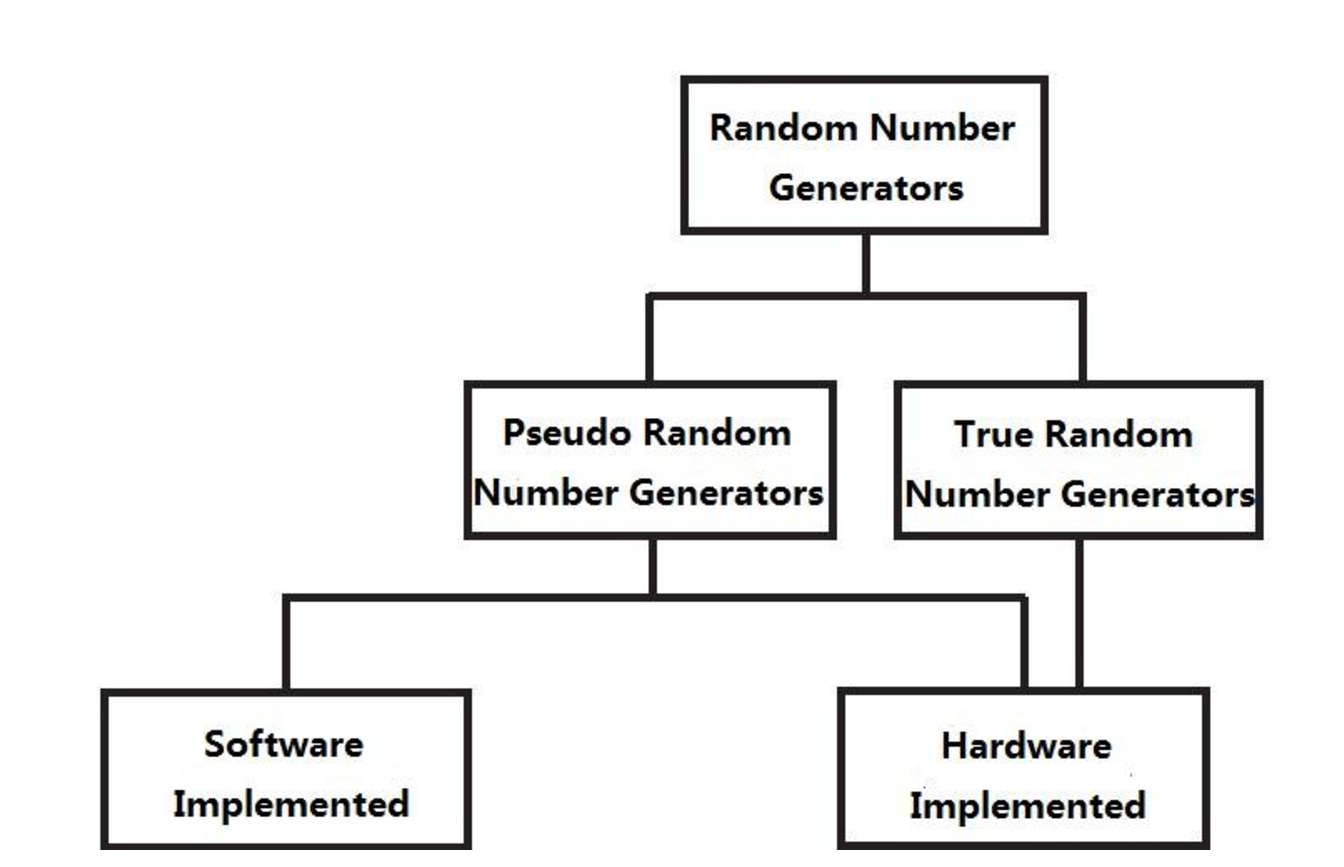
\includegraphics[width=3.85in]{Classification.eps}
\DeclareGraphicsExtensions.
\caption{Classification of random number generators}
\label{Classification}
\end{figure}



\subsection{True Random Number Generators (TRNGs)}
A TRNG is a physical device that generates statistically independent and unbiased bits. They are also
called non-deterministic RNGs. Such devices, which
exist too in computers, are often based on microscopic phenomena that generate a low-level, statistically random ``noise'' signal, such as thermal noise, photoelectric effect, or any other quantum phenomena. These processes are, in theory, completely unpredictable, and the theory's assertions of unpredictability are subject to experimental test. 

A quantum-based hardware random number generator typically consists in a transducer that converts some aspect of a given physical phenomena, into an electrical signal. An amplifier and other electronic circuitry bring the output of the transducer into the macroscopic realm, and some analog to digital converter translates the output into a digital number, often a simple binary digit 0 or 1. By repeatedly sampling the randomly varying signal, a series of random numbers is thus obtained.

\subsection{Pseudo Random Number Generators (PRNGs)}

A pseudorandom number generator (PRNG), also known as deterministic random bit generator (DRBG), is an algorithm for generating a sequence of numbers that approximates the properties of random numbers~\cite{Barker05recommendationfor}. The sequence is not truly random in that it is completely determined by a relatively small set of initial values, called the PRNG's state. Although sequences that are closer to truly random can be generated using hardware random number generators, pseudorandom numbers are important in practice for simulations (e.g., of physical systems with the Monte Carlo method), and are central in   cryptography and procedural generation due to their fundamental property of reproductibility. 

Common classes of these algorithms are linear congruential generators, Lagged Fibonacci generators, linear feedback shift registers, feedback with carry shift registers, and generalized feedback shift registers. Recent instances of pseudorandom algorithms include Blum Blum Shub, Fortuna, and the Mersenne twister.
All these generators will be developed later in this manuscript.

%\section{Cryptographically secure pseudo random number generators}
%
%
%A PRNG suitable for cryptographic applications is called a cryptographically secure PRNG (CSPRNG). A requirement for a CSPRNG is that an adversary not knowing the seed has only negligible advantage in distinguishing the generator's output sequence from a random sequence. In other words, while a PRNG is only required to pass certain statistical tests, a CSPRNG must pass all statistical tests that are restricted to polynomial time in the size of the seed. Though such property cannot be proven, strong evidence may be provided by reducing the CSPRNG to a known hard problem in mathematics (e.g., integer factorization). In general, years of review may be required before an algorithm can be certified as a CSPRNG.
%
%Some classes of CSPRNGs include the following:
%\begin{itemize}
%
%\item     Stream ciphers
%\item     Block ciphers running in counter or output feedback mode.
%\item     PRNGs that have been designed specifically to be cryptographically secure, such as Microsoft's Cryptographic 
% Application Programming Interface function CryptGenRandom, the Yarrow algorithm (incorporated in Mac OS X and FreeBSD), and Fortuna.
%\item     Combination PRNGs which attempt to combine several PRNG primitive algorithms with the goal of removing any non-randomness.
%\item     Special designs based on mathematical hardness assumptions. Examples include Micali-Schnorr and the Blum Blum Shub algorithm, which provide a strong security proof. Such algorithms are rather slow compared to traditional constructions, and impractical for many applications.
% 
%\end{itemize}

%\section{Stream Cipher}
%A stream cipher generates successive elements of the keystream based on an internal state. This state is updated in essentially two ways: if the state changes independently of the plaintext or ciphertext messages, the cipher is classified as a synchronous stream cipher. By contrast, self-synchronising stream ciphers update their state based on previous ciphertext digits.
%
%\subsection{One-Time Pad (Vernam Cipher)}
%In modern terminology, a Vernam cipher is a stream cipher in which the plaintext is XORed with a random or pseudorandom stream of data (the keystream) of the same length to generate the ciphertext. If the keystream is truly random and used only once, this is effectively a one-time pad. 
%
%Shannon~\cite{shannon-otp} showed that the one-time pad provides perfect security. This means
%that the conditional entropy of the message $M$ knowing the ciphertext $C$ is the same as the
%entropy of the original message, i.e. $H(M|C) = H(M)$. He also showed that the one-time
%pad is optimal in the sense that the previous conditions cannot be achieved with a key of
%size smaller than the message.
%
%The problem of the one-time pad is that we first have to agree on a key of the same
%length as the message. For most applications this is not practical. The next two schemes
%try to produce a ``random looking`` keystream from a short key and IV. By random looking,
%we mean that we cannot distinguish the keystream from a random sequence in a complexity
%less than trying all possible keys.
%
%\subsection{Synchronous stream ciphers}
%In a synchronous stream cipher a stream of pseudorandom digits is generated independently of the plaintext and ciphertext messages, and then combined with the plaintext (to encrypt) or the ciphertext (to decrypt). In the most common form, binary digits are used (bits), and the keystream is combined with the plaintext using the exclusive or operation (XOR). This is termed a binary additive stream cipher.
%
%In a synchronous stream cipher, the sender and receiver must be exactly in step for decryption to be successful. If digits are added or removed from the message during transmission, synchronisation is lost. To restore synchronisation, various offsets can be tried systematically to obtain the correct decryption. Another approach is to tag the ciphertext with markers at regular points in the output.
%
%If, however, a digit is corrupted in transmission, rather than added or lost, only a single digit in the plaintext is affected and the error does not propagate to other parts of the message. This property is useful when the transmission error rate is high; however, it makes it less likely the error would be detected without further mechanisms. Moreover, because of this property, synchronous stream ciphers are very susceptible to active attacks -- if an attacker can change a digit in the ciphertext, he might be able to make predictable changes to the corresponding plaintext bit; for example, flipping a bit in the ciphertext causes the same bit to be flipped in the plaintext.
%
%\subsection{Self-synchronizing stream ciphers}
%Another approach uses several of the previous N ciphertext digits to compute the keystream. Such schemes are known as self-synchronizing stream ciphers, asynchronous stream ciphers or ciphertext autokey (CTAK). The idea of self-synchronization was patented in 1946, and has the advantage that the receiver will automatically synchronise with the keystream generator after receiving N ciphertext digits, making it easier to recover if digits are dropped or added to the message stream. Single-digit errors are limited in their effect, affecting only up to N plaintext digits.
%
%An example of a self-synchronising stream cipher is a block cipher in cipher feedback (CFB) mode.
%


\subsection{Chaos-based Random Number Generators}

Since the seventies in last century, the use of chaotic dynamics for the generation of random sequences has raised a lot of interests. It is clearly pointed out by some researchers that there exists a close relationship between chaos and randomness, and many works have been witnessed in the last two decades~\cite{Provenzale199231}.
To do so, chaotic dynamics are usually studied in two different domains, depending on whether the generator is an hardware or a software one.
\begin{itemize}
 \item Continuous time domain: chaotic dynamics generated by differential equations.
 \item Discrete time domain: recurrent sequences using chaotic maps.
\end{itemize}

Chaos possesses several distinct properties that can possibly give meaning to the desire to use such dynamics for generating pseudorandomness, namely: the sensitivity to initial conditions, the ergodicity, the wide band spectrum, and the unpredictable and random-like behavior of iterates.
Although it is still controversy to equate these properties with randomness and claim a chaos-based random number generator to be good enough, a lot of designs and applications, in particular related to communications securing, have been proposed.

Nowadays, it is common to use a chaotic map for pseudorandom number generation. Due to the recent design of electronic circuits for the realization of chaotic systems, it is also possible to generate the bit sequence by observing such dynamics, as a replacement of those physical random sources.

\section{Statistical Tests for Randomness}
\label{Some famous statistical tests of random number generators}

A theoretical proof for the randomness of a generator is impossible to give, as such proof requires first to mathematically define what is randomness. Therefore statistical inference based on observed sample sequences produced by the generator seems to be the best option. Considering the properties of binary
random sequences, various statistical tests can be designed to evaluate the assertion
that the sequence is generated by a perfectly random source. 
We have performed certain statistical tests for various CI PRNGs we proposed. These tests
include TestU01~\cite{Lecuyer2009}, NIST suite~\cite{ANDREW2008},
DieHARD battery of tests~\cite{Marsaglia1996}, and Comparative test parameters. For completeness and for reference, we give
in the following subsection a brief description of each of the
aforementioned tests.



\subsection{NIST statistical test suite}



Among the numerous standard tests for pseudo-randomness, a convincing way to show the randomness of the produced sequences is to confront them to the NIST (National Institute of Standards and Technology) Statistical Test, because it is an up-to-date test suite proposed by the Information Technology Laboratory (ITL). A new version of the Statistical Test Suite (Version 2.0) has been released in August 11, 2010.


The NIST test suite SP 800-22 is a statistical package consisting of 15 tests. They were developed to test the randomness of binary sequences produced by hardware or software based cryptographic PRNGs. These tests focus on a variety of different types of non-randomness that could exist in a sequence. 


For each statistical test, a set of $p-values$ (corresponding to the set of sequences) is produced. The interpretation of empirical results can be conducted in any number of ways. In this manuscript, the examination of the distribution of $p-values$ to check for uniformity ($p-value_{T}$) is used:
the distribution of $P-values$ is examined to ensure uniformity. 
Concretely, this demand is verified in an usual way as follows: if $p-value_{T} \geqslant 0.0001$, then the sequences can be considered to be uniformly distributed.

In our experiments, 100 sequences (s = 100), each with 1,000,000-bit long, are generated and tested. If the $p-value_{T}$ of any test is smaller than 0.0001, the sequences are considered to be not good enough and the generating algorithm is not suitable for usage.

In what follows, the fifteen tests of the NIST Statistical tests suite, are recalled. A more detailed description for those tests could be found in \cite{ANDREW2008}.
\begin{itemize}
\item \textbf{Frequency (Monobit) Test (FT)} is to determine whether the number of ones and zeros in a sequence are approximately the same as would be expected for a truly random sequence.


\item \textbf{Frequency Test within a Block (FBT)} is to determine whether the frequency of ones in an M-bit block is approximately $M/2$, as would be expected under an assumption of randomness. %($M$ is the length of each block.)


\item \textbf{Runs Test (RT)} is to determine whether the number of runs of ones and zeros of various lengths is as expected for a random sequence. In particular, this test determines whether the oscillation between such zeros and ones is too fast or too slow.


\item \textbf{Test for the Longest Run of Ones in a Block (LROBT)} is to determine whether the length of the longest run of ones within the tested sequence is consistent with the length of the longest run of ones that would be expected in a random sequence.


\item \textbf{Binary Matrix Rank Test (BMRT)} is to check for linear dependence among fixed length substrings of the original sequence.


\item \textbf{Discrete Fourier Transform (Spectral) Test (DFTT)} is to detect periodic features (i.e., repetitive patterns that are near each other) in the tested sequence that would indicate a deviation from the assumption of randomness.


\item \textbf{Non-overlapping Template Matching Test (NOTMT)} is to detect generators that produce too many occurrences of a given non-periodic (aperiodic) pattern.


\item \textbf{Overlapping Template Matching Test (OTMT)} is to check the number of occurrences of pre-specified target strings.

\item \textbf{Maurer's ``Universal Statistical'' Test (MUST)} is to detect whether or not the sequence can be
significantly compressed without loss of information.

\item \textbf{Linear Complexity Test (LCT)} is to determine whether or not the sequence is complex enough to be considered random.

\item \textbf{Serial Test (ST)} is to determine whether the number of occurrences of the $2^{m}$ $m$-bit
overlapping patterns is approximately the same as would be expected for a random sequence.

\item \textbf{Approximate Entropy Test (AET)} is to compare the frequency of overlapping blocks of two consecutive/adjacent lengths (m and m+1) against the expected result for a random sequence.%(m is the length of each block.)

\item \textbf{Cumulative Sums (Cusum) Test (CST)} is to determine whether the cumulative sum of the partial sequences occurring in the tested sequence is too large or too small relative to the expected behavior of that cumulative sum for random sequences.

\item \textbf{Random Excursions Test (RET)} is to determine if the number of visits to a particular state within a cycle deviates from what one would expect for a random
sequence.

\item \textbf{Random Excursions Variant Test (REVT)} is to detect deviations from the expected number
of visits to various states in the random walk.
\end{itemize}

\subsection{DieHARD battery of tests}
The DieHARD battery of tests was developed in 1996 by Prof. Georges Marsaglia
from the Florida State University for testing randomness of sequences of numbers \cite{Marsaglia1996}. 
It has been the most sophisticated standard for over a decade. Because of the stringent requirements in the DieHARD test suite, a generator passing DieHARD battery of 
tests can be considered good as a rule of thumb. It was supposed to give a better way of analysis in comparison to original FIPS statistical tests.

The DieHARD battery of tests consists of 18 different independent statistical tests. 
Each test requires binary file of about 10-12 million bytes in order to run the full set of tests. 
As the NIST test suite, most of the tests in DieHARD return a $p-value$, which should be uniform on $[0,1)$ if the input file 
contains truly independent random bits. Those $p-values$ are obtained by
$p=F(X)$, where $F$ is the assumed distribution of the sample random variable $X$ (often normal). 
But that assumed $F$ is just an asymptotic approximation, for which the fit will be worst 
in the tails. Thus occasional $p-value$s near 0 or 1, such as 0.0012 or 0.9983 can occur. Unlike the NIST test suite, the test is considered to be successful when
the $p-value$ is in range $[0 + \alpha , 1 -\alpha ]$,
where $\sqrt{\alpha}$ is the level of significance of the test.

For example, with a level of significance of $5\%$, $p-values$ are expected to be in
$[0.025, 0.975]$. Note that if the $p-value$ is not in this range, it means that the null
hypothesis for randomness is rejected even if the sequence is truly random. These
tests are:
\begin{itemize}
\item \textbf{Birthday Spacings.} Choose random points on a large interval. The spacings
between the points should be asymptotically Poisson distributed. The name
is based on the birthday paradox.
\item \textbf{Overlapping Permutations.} Analyze sequences of five consecutive random
numbers. The 120 possible orderings should occur with statistically equal
probability
\item \textbf{Ranks of matrices.} Select some number
of bits from some number of random numbers to form a matrix over 0,1, then
determine the rank of the matrix. Count the ranks.
\item \textbf{Monkey Tests.} Treat sequences of some number of bits as ``words''. Count
the overlapping words in a stream. The number of ``words'' that don't appear
should follow a known distribution. The name is based on the infinite monkey
theorem.
\item \textbf{Count the 1's.} Count the 1 bits in each of either successive
or chosen bytes. Convert the counts to ``letters'', and count the occurrences
of five-letter ``words''
\item \textbf{Parking Lot Test.} Randomly place unit circles in a $100 \times 100 $ square. If the
circle overlaps an existing one, try again. After 12,000 tries, the number of
successfully ``parked'' circles should follow a certain normal distribution.
\item \textbf{Minimum Distance Test.} Randomly place 8,000 points in a $10,000 \times 10,000$ 
square, then find the minimum distance between the pairs. The square of this
distance should be exponentially distributed with a certain mean.
\item \textbf{Random Spheres Test.} Randomly choose 4,000 points in a cube of edge 1,000.
Center a sphere on each point, whose radius is the minimum distance to another point. The smallest sphere's volume should be exponentially distributed
with a certain mean.
\item \textbf{The Sqeeze Test.} Multiply 231 by random floats on [0,1) until you reach 1.
Repeat this 100,000 times. The number of floats needed to reach 1 should
follow a certain distribution.
\item \textbf{Overlapping Sums Test.} Generate a long sequence of random floats on [0,1).
Add sequences of 100 consecutive floats. The sums should be normally distributed with characteristic mean and sigma.
\item \textbf{Runs Test.} Generate a long sequence of random floats on [0,1). Count ascending and descending runs. The counts should follow a certain distribution.
\item \textbf{The Craps Test.} Play 200,000 games of craps, counting the wins and the number
of throws per game. Each count should follow a certain distribution.
\end{itemize}

\subsection{ENT test program}
%
ENT test program applies various tests to sequences of bytes stored in
files and reports the results of those tests. The program is useful
for evaluating random number generators for encryption and statistical
sampling applications, compression algorithms, and other applications
where the information density of a file is of interest~\cite{ent}.

There are 5 tests contained in the program:
%
\begin{enumerate}
\item Entropy test: Entropy testing, in bits per character (or byte), which
  corresponds to the incompressibility of the sequence (as a perfectly
  random sequence cannot be compressed, since no part of it can be
  expressed in terms of other parts). Hence entropy of 8 bits/byte
  means perfect randomness in the sense of incompressibility.
\item $\chi^2$ test: $\chi^2$ testing is very common for
  goodness-of-fit of sample distributions of random numbers. It is
  known to be very sensitive to deficiencies in random number
  generators (when it is located between 5\% to 95\%, data are treated
  as random).
\item Sample test: Sample test means can be tested for bias in random
  number generation. In binary mode, the expected mean is 0.5 while
  for bytes, the expected mean is 127.5.
\item Monte Carlo test: a Monte Carlo approximation of $\pi$, which is
  simply the evaluation the area of the unit circle using the $N$
  generated random numbers ($X_i$,$X_{i-1}$), $i = 2,...,N$.
\item Serial Correlation test: Serial correlation coefficient
  evaluated from $<X_i,X_{i-1}>/<X_i,X_i>$, for $i=2,..N$. The
  intended value for perfect random sequences is 0.
\end{enumerate}

\subsection{Comparative test parameters}

In this section, five well-known statistical tests~\cite{Menezes1997} are presented to play the role of easily verifiable comparison tools. They encompass frequency and autocorrelation tests. In what follows, $s = s^0,s^1,s^2,\dots , s^{n-1}$ denotes a binary sequence of length $n$. The question is to determine whether this sequence possesses some specific characteristics that a truly random sequence would be likely to exhibit. 


\paragraph{Frequency test (monobit test)}

The purpose of this test is to check if the numbers of 0's and 1's are approximately equal in $s$, as it would be expected for a random sequence. Let $n_0, n_1$ denote these numbers. The statistic used here is 
\begin{equation*}
X_1=\frac{(n_0-n_1)^2}{n}, 
\end{equation*}
which approximately follows a $\chi^2$ distribution with one degree of freedom when $n\geqslant 10^7$.

\paragraph{Serial test (2-bit test)}

The purpose of this test is to determine if the number of occurrences of 00, 01, 10, and 11 as subsequences of $s$ are approximately the same. Let $n_{00} , n_{01} ,n_{10}$, and $n_{11}$ denote the number of occurrences of $00, 01, 10$, and $11$ respectively. Note that $n_{00} + n_{01} + n_{10} + n_{11} = n-1$ since the subsequences are allowed to overlap. The
statistic used here is:
\begin{equation*}
X_2=\frac{4}{n-1}(n_{00}^2+n_{01}^2+n_{10}^2+n_{11}^2)-\frac{2}{n}(n_0^2+n_1^2)+1,
\end{equation*}
 which approximately follows a $\chi^2$ distribution with 2 degrees of freedom if $n\geqslant 21$.

\paragraph{Poker test}

The poker test studies if each pattern of length $m$ (without overlapping) appears the same number of times in $s$. Let $\lfloor \frac{n}{m} \rfloor\geqslant 5 \times 2^m$ and $k= \lfloor \frac{n}{m} \rfloor $. Divide the sequence $s$ into $k$ non-overlapping parts, each of length $m$. Let $n_i$ be the number of occurrences of the $i^{th}$ type of sequence of length $m$, where $1 \leqslant i \leqslant 2^m$. The statistic used is 
\begin{equation*}
X_3=\dfrac{2^m}{k}\left(\displaystyle{\sum^{2^m}_{i=1}n^2_i}\right)-k,
\end{equation*}
which approximately follows a $\chi^2$ distribution with $2^m-1$ degrees of freedom. Note that the poker test is a generalization of the frequency test (setting $m = 1$ in the poker test yields the frequency test).

\paragraph{Runs test}

The purpose of the runs test is to figure out whether the number of runs of various lengths in the sequence $s$ is as expected, for a random sequence. A run is defined as a pattern of all zeros or all ones, a block is a run of ones, and a gap is a run of zeros. The expected number of gaps (or blocks) of length $i$ in a random sequence of length $n$ is $e_i = \frac{n-i+3}{2^{i+2}}$. Let $k$ be equal to the largest integer $i$ such that $e_i \geqslant 5$. Let
$B_i , G_i$ be the number of blocks and gaps of length $i$ in $s$, for each $i \in \llbracket 1, k\rrbracket$. The statistic used here will then be:
\begin{equation*}
\displaystyle{X_4=\sum^k_{i=1}\frac{(B_i-e_i)^2}{e_i}+\sum^k_{i=1}\frac{(G_i-e_i)^2}{e_i}},
\end{equation*}
\noindent which approximately follows a $\chi^2$ distribution with $2k - 2$ degrees of freedom.

\paragraph{Autocorrelation test}

The purpose of this test is to check for coincidences between the sequence $s$ and (non-cyclic) shifted versions of it. Let $d$ be a fixed integer, $ 1 \leqslant d \leqslant \lfloor n/2 \rfloor$. The value $A(d) = \sum_{i=0}^{n-d-1} s_i\oplus s_{i+d}$ is the amount of bits not equal between the sequence and itself displaced by $d$ bits. The statistic used is:
\begin{equation*}
X_5=\dfrac{2 \left(A(d)-\frac{n-d}{2}\right)}{\sqrt{n-d}},
\end{equation*}
which approximately follows a normal distribution $\mathcal{N}(0, 1)$ if $n-d \geqslant 10$. Since small values of $A(d)$ are as unexpected as large values, a two-sided test should be used.

\subsection{TestU01 Statistical Test}
\label{Testing a generator}

TestU01 is extremely diverse in implementing classical tests,
cryptographic tests, new tests proposed in the literature, and original tests.
In fact, it encompasses most of the other testsuites. 
There are seven batteries of tests in the TestU01 package, which are listed in what follows:

\begin{itemize}
\item{\textbf{SmallCrush.}} The first battery to check, with 15 $p-$values reported. This is a fast collection of tests used to be sure that the basic requirements of randomness are satisfied. In case of success, this battery should be followed by Crush and BigCrush.
\item{\textbf{Crush.}} This battery includes many difficult tests, like those described in~\cite{Knuth1998}. %Cette référence n'apparaît pas.
%D. E. Knuth. The Art of Computer Programming, Volume 2: Seminumerical Algorithms. Addison-Wesley, Reading, Mass., third edition, 1998.
It uses approximately $2^{35}$ random numbers and applies 96 statistical tests
(it computes a total of 144 test statistics and $p-values$).
\item{\textbf{BigCrush.}} The BigCrush uses
approximately $2^{38}$ random numbers and applies 106 tests (it computes 160 test
statistics and $p-values$). 
A suite of very stringent statistical tests, and the most difficult battery to pass.
\item{\textbf{Rabbit.}} This battery of tests reports 38 $p-values$.
\item{\textbf{Alphabit.}} Alphabit and AlphabitFile have been designed primarily to test hardware random bits generators. 17 $p-values$ are reported here.
\item{\textbf{Pseudo-DieHARD.}} This battery implements most of the tests contained in the popular battery DieHARD or, in some cases, close approximations to them. It is not a very stringent battery. Indeed, there is no generator that can pass Crush and BigCrush batteries and fail Pseudo-DieHARD, while the converse occurs for several defective generators. 126 $p-values$ are reported here.
\item{\textbf{FIPS\_140\_2.}} As recalled previously, the NIST (National Institute of Standards and Technology) of the U.S. federal government has proposed a statistical test suite. It is used to evaluate the randomness of bitstreams produced by cryptographic random number generators. This battery reports 16 $p-values$.
\end{itemize}

Six predefined batteries of tests are available in TestU01; three of them
are for sequences of $\mathcal{U}(0, 1)$ random numbers and the three others are for bit
sequences. In the first category, we have SmallCrush, Crush, and BigCrush.

To test a RNG for general use,
one could first apply the small and fast battery SmallCrush. If it passes, one could then apply
the more stringent battery Crush, and finally the yet more time-consuming battery BigCrush.
These batteries of tests include the classical tests described in Knuth~\cite{Knuth1998}, for
example: the run, poker, coupon collector, gap, max-of-t, and permutation tests.
There are collision and birthday spacings tests in 2, 3, 4, 7, 8 dimensions, several close pairs tests in 2, 3, 5, 7, 9 dimensions, and correlation tests. Some
tests use the generated numbers as a sequence of ``random'' bits: random walk
tests, linear complexity tests, a Lempel-Ziv compression test, several Hamming
weights tests, matrix rank tests, run and correlation tests, among others.




The batteries Rabbit, Alphabit, and BlockAlphabit are for binary sequences
(e.g., a cryptographic pseudorandom generator or a source of random bits
produced by a physical device). They were originally designed to test a finite
sequence contained in a binary file. When invoking the battery, one must specify the number $n_B$ of bits available for each test. When the bits are in a file, $n_B$
must not exceed the number of bits in the file, and each test will reuse the same
sequence of bits starting from the beginning of the file (so the tests are not independent). When the bits are produced by a generator, each test uses a different
stream. In both cases, the parameters of each test are chosen automatically as
a function of $n_B$ .
The batteries Alphabit and Rabbit can be applied on a binary file considered as a source
of random bits. They can also be applied on a programmed generator. Alphabit has been
defined primarily to test hardware random bits generators. The battery PseudoDieHARD
applies most of the tests in the well-known DieHARD suite of Marsaglia [106]. The battery
FIPS\_140\_2 implements the small suite of tests of the FIPS\_140\_2 standard from NIST.
The batteries described in this module will write the results of each test (on standard
output) with a standard level of details (assuming that the Boolean switches of module
swrite have their default values), followed by a summary report of the suspect p-values
obtained from the specific tests included in the batteries. It is also possible to get only the
summary report in the output, with no detailed output from the tests, by setting the Boolean
switch swrite\_Basic to FALSE. Rabbit and Alphabit apply 38 and 17 different statistical tests,
respectively. 

Some of the tests compute more than one statistic (and $p-value$) using the same stream of random
numbers and these statistics are thus not independent. That is why the number of statistics
in the summary reports is larger than the number of tests in the description of the batteries.
For a more detailed description, the reader is referred
to the documentation of the TestU01 library.

\begin{itemize}
\item{\textbf{Small Crush:}}\\smarsa\_BirthdaySpacings \\ 
 sknuth\_Collision \\ 
 sknuth\_Gap\\ 
 sknuth\_SimpPoker \\ 
 sknuth\_CouponCollector\\ 
 sknuth\_MaxOft \\ 
 svaria\_WeightDistrib \\ 
 smarsa\_MatrixRank \\
 sstring\_HammingIndep\\ 
 swalk\_RandomWalk1\\ 
\item{\textbf{Crush:}}\\smarsa\_SerialOver \\
 smarsa\_CollisionOver\\ 
 smarsa\_BirthdaySpacings\\ 
 snpair\_ClosePairs\\ 
 snpair\_ClosePairsBitMatch \\
 sknuth\_SimpPoker\\ 
 sknuth\_CouponCollector\\ 
 sknuth\_Gap\\ 
 sknuth\_Run\\ 
 sknuth\_Permutation\\ 
 sknuth\_CollisionPermut\\ 
 sknuth\_MaxOft\\ 
 svaria\_SampleProd\\ 
 svaria\_SampleMean \\ 
 svaria\_SampleCorr\\ 
 svaria\_AppearanceSpacings \\
 svaria\_WeightDistrib \\
 svaria\_SumCollector\\ 
 smarsa\_MatrixRank\\ 
 smarsa\_Savir2\\ 
 smarsa\_GCD\\ 
 swalk\_RandomWalk1\\ 
 scomp\_LinearComp \\
 scomp\_LempelZiv\\ 
 sspectral\_Fourier3\\ 
 sstring\_LongestHeadRun \\
 sstring\_PeriodsInStrings\\ 
 sstring\_HammingWeight2\\ 
 sstring\_HammingCorr\\ 
 sstring\_HammingIndep \\
 sstring\_Run\\ 
 sstring\_AutoCor \\ 
\item{\textbf{Big Crush:}}\\smarsa\_SerialOver\\ 
smarsa\_CollisionOver\\ 
smarsa\_BirthdaySpacings\\ 
snpair\_ClosePairs \\ 
sknuth\_SimpPoker\\ 
sknuth\_CouponCollector\\ 
sknuth\_Gap\\ 
sknuth\_Run\\ 
sknuth\_Permutation\\ 
sknuth\_CollisionPermut\\ 
sknuth\_MaxOft\\ 
svaria\_SampleProd\\ 
svaria\_SampleMean\\ 
svaria\_SampleCorr\\ 
svaria\_AppearanceSpacings\\ 
svaria\_WeightDistrib\\ 
svaria\_SumCollector\\ 
smarsa\_MatrixRank\\ 
smarsa\_Savir2\\ 
smarsa\_GCD\\ 
swalk\_RandomWalk1\\ 
scomp\_LinearComp\\ 
scomp\_LempelZiv\\ 
sspectral\_Fourier3\\ 
sstring\_LongestHeadRun\\ 
sstring\_PeriodsInStrings\\ 
sstring\_HammingWeight2\\ 
sstring\_HammingCorr\\ 
sstring\_HammingIndep\\ 
sstring\_Run\\ 
sstring\_AutoCor\\ 

\item{\textbf{Rabbit:}}\\smultin\_MultinomialBitsOver\\ 
snpair\_ClosePairsBitMatch\\ 
svaria\_AppearanceSpacings\\ 
scomp\_LinearComp\\ 
scomp\_LempelZiv\\ 
sspectral\_Fourier1\\ 
sspectral\_Fourier3\\ 
sstring\_LongestHeadRun\\ 
sstring\_PeriodsInStrings\\ 
sstring\_HammingWeight\\ 
sstring\_HammingCorr\\ 
sstring\_HammingIndep\\ 
sstring\_AutoCor\\ 
sstring\_Run\\ 
smarsa\_MatrixRank\\ 
swalk\_RandomWalk1\\ 

\item{\textbf{Alphabit:}}\\smultin\_MultinomialBitsOver\\ 
sstring\_HammingIndep\\ 
sstring\_HammingCorr\\ 
swalk\_RandomWalk1 \\ 


\item{\textbf{Pseudo-DieHARD:}}\\Birthday Spacings test\\ 
Overlapping 5-Permutation test\\ 
Binary Rank Tests for Matrices test\\ 
Bitstream test\\ 
OPSO test\\ 
OQSO test\\ 
DNA test\\ 
Count-the-1's test\\ 
Parking Lot test\\ 
Minimum Distance test\\ 
3-D Spheres test\\ 
Squeeze test\\ 
Overlapping Sums test\\ 
Runs test\\ 
Craps test\\ 

\item{\textbf{FIPS\_140\_2:}}\\Monobit test\\ 
``poker'' test\\ 
Runs test\\ 
Longest Run of Ones in a Block test

\end{itemize}

TestU01 suite implements hundreds of tests and reports $p-$values. If a $p-$value is within $[0.001,0.999]$, the associated test is a success. A $p-$value lying outside this boundary means that its test has failed. %This is the standard range the test-suite suggests. The p-value selection criteria for the various test suites were chosen to produce a few failures in the best cases. Setting the criteria too low (closer to zero) would exhibit no failures and setting the criteria too high would fail everything.




\section{FPGA}
We finally introduce the field-programmable gate array (FPGA) architecture, on which our generators will be
implemented. 

A FPGA is an integrated circuit designed to be configured by a customer or a designer after manufacturing-hence ``field-programmable'' 
\begin{figure}
\centering
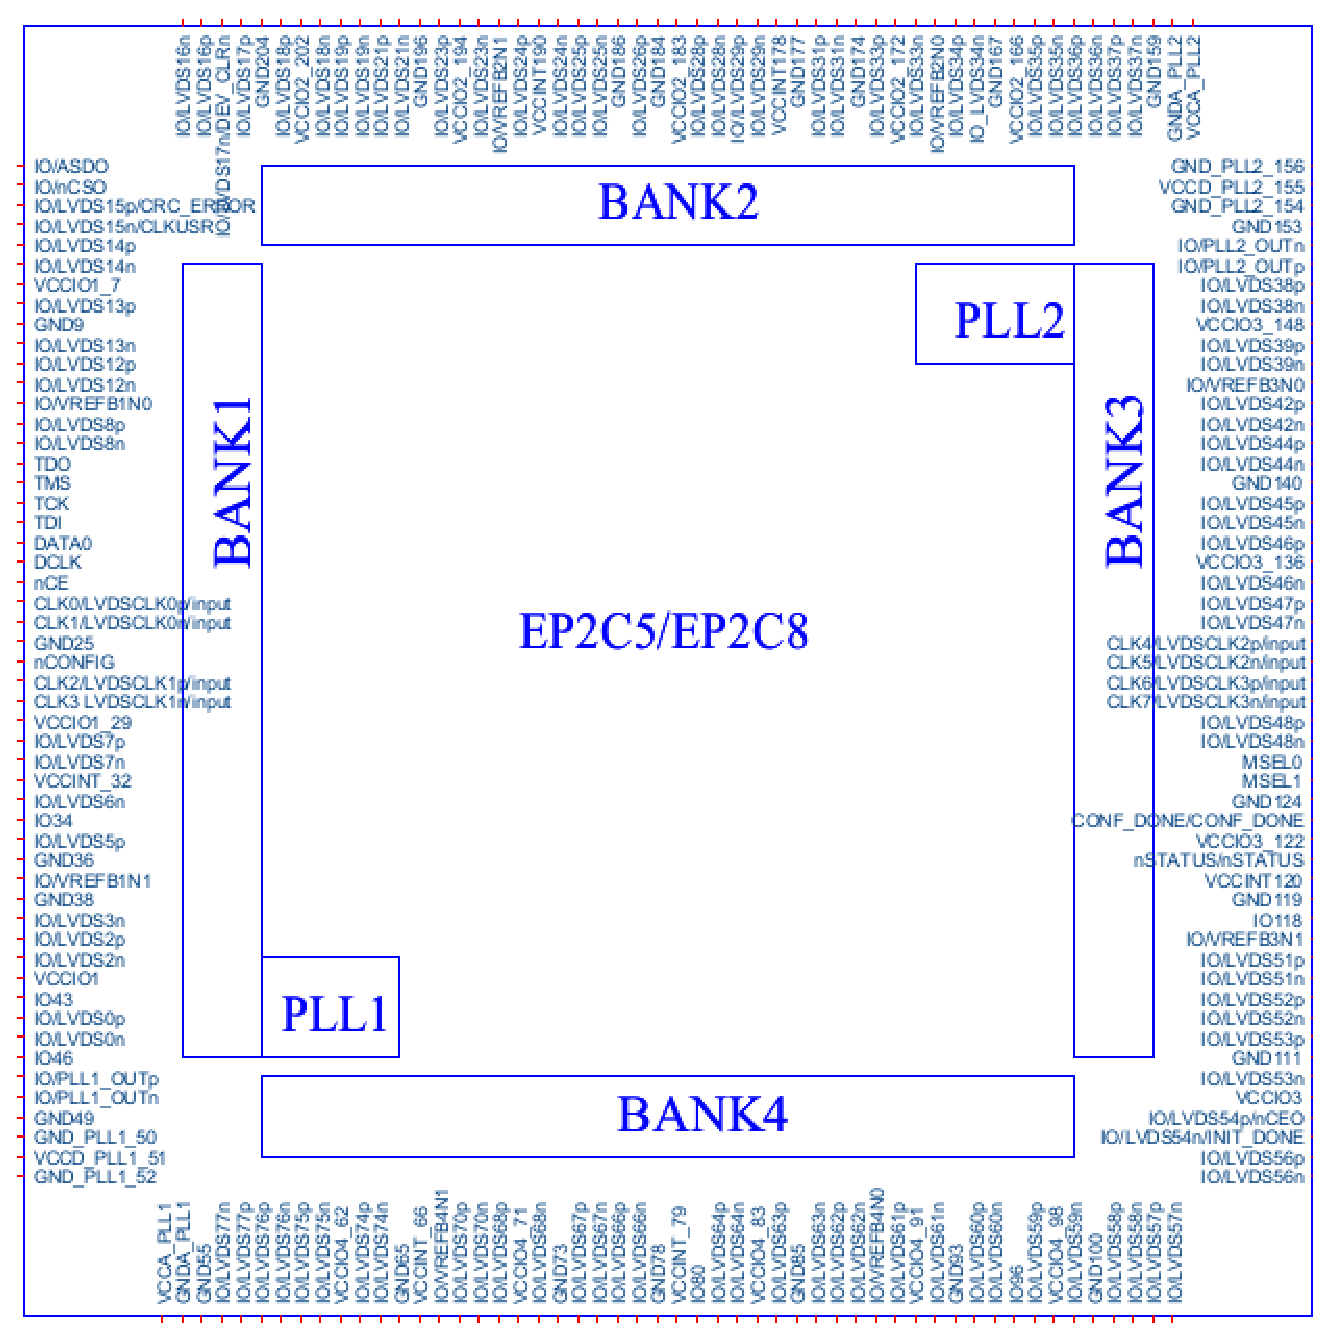
\includegraphics[width=5in]{fpga_scheme.eps}
\DeclareGraphicsExtensions.
\caption{FPGA EP2C8 core from ALTERA company}
\label{fpga_scheme}
\end{figure}
%The experiments in this research were implemented on FPGA. 
(a FPGA is indeed a VLSI chip with some special features).
The most common FPGA architecture consists of an array of logic blocks (called Configurable Logic Block, CLB, or Logic Array Block, LAB, depending on vendor), I/O pads, and routing channels. Generally, all the routing channels have the same width (number of wires). Multiple I/O pads may fit into the height of one row or the width of one column in the array. There are some primitives such as lookup tables (LUT) and flip-flop (FF) inside the CLB. The functions of these primitives and connections between them can be configured for different designs. Programmable routing matrices (PRM), implemented in static RAMs, are used to connect the I/O ports of the CLBs.

The advantages of FPGA designs over traditional VLSI designs are:
\begin{itemize}
\item The feasibility of reusing fast design to product time and chips for different designs.
\item Easy simulation and debugging. Software simulator and debugger provide
efficient methods of finding bugs and estimating of performance.
\item Low cost prototyping for early designs.
\item Design can be upgraded after deployment without hardware replacement.
\item Developing  hardware  systems  using  design  tools  for  FPGA  is  as  easy  as developing a software system.
\item FPGA can be reprogrammed on the field. 
\end{itemize}

To define the behavior of the FPGA, the user provides a hardware description language (HDL) or a schematic design. The most common HDLs are VHDL and Verilog, although in an attempt to reduce the complexity of designing in HDLs, which have been compared to the equivalent of assembly languages, there are moves to raise the abstraction level through the introduction of alternative languages. 

A general structure outline of FPGA core (EP2C8) used in this thesis is shown in Fig.\ref{fpga_scheme}



\part{First Part: Pseudo Random Number Generator Based on Chaotic Iteration}
\chapter{General Notions}
\label{General Notions}
\minitoc
 
This chapter, serving as the background of this thesis,  
is devoted to basic notations and terminologies in the fields of random number and its classification.


\section{Randomness}
A random bit sequence could be interpreted as the result of the flips of an unbiased "fair" coin with sides
that are labeled "0" and "1," with each flip having a probability of exactly $1/2$ of producing a "0" or "1."
Furthermore, the flips are independent of each other: the result of any previous coin flip does not affect
future coin flips. The unbiased "fair" coin is thus the perfect random bit stream generator, since the "0"
and "1" values will be randomly distributed (and [0,1] uniformly distributed). All elements of the
sequence are generated independently of each other, and the value of the next element in the sequence
cannot be predicted, regardless of how many elements have already been produced.
Obviously, the use of unbiased coins for cryptographic purposes is impractical. Nonetheless, the
hypothetical output of such an idealized generator of a true random sequence serves as a benchmark for
the evaluation of random and pseudorandom number generators.~\cite{ANDREW2008}

\section{Types of Random Number Generators (RNGs)}
A RNG is a computational or physical device designed to generate a sequence of numbers or symbols that lack any pattern, i.e. appear random.

It is always a difficult task to generate good random number/sequence. Although it is accepted that rolling a dice or drawing cards is random these mechanical methods are not practical. in the past, random numbers are usually generated offline based on some dedicated setup or devices, and the sequences are stored in table ready for use. These random tables are still available in the world-wide-web or some data CDROMs.

However, due to the online requirements and the security issues, random table becomes inappropriate, and hence different RNGs have been proposed, especially after the introduction of computer.

In general, RNGs can be grouped into two classes, namely true random number gernerators and pseudo random number generators, depending on their sources of randomness. 
RNGs can be classified as:
\subsection{True Random Number Generators (TRNGs)}
A TRNG is one which generates statistically independent and unbiased bits. These are also
called as non-deterministic RNGs. In computing, a True random number generator is an apparatus that generates random numbers from a physical process. Such devices are often based on microscopic phenomena that generate a low-level, statistically random "noise" signal, such as thermal noise or the photoelectric effect or other quantum phenomena. These processes are, in theory, completely unpredictable, and the theory's assertions of unpredictability are subject to experimental test. A quantum-based hardware random number generator typically consists of a transducer to convert some aspect of the physical phenomena to an electrical signal, an amplifier and other electronic circuitry to bring the output of the transducer into the macroscopic realm, and some type of analog to digital converter to convert the output into a digital number, often a simple binary digit 0 or 1. By repeatedly sampling the randomly varying signal, a series of random numbers is obtained.

\subsection{Pseudo Random Number Generators (PRNGs)}
A pseudorandom number generator (PRNG), also known as a deterministic random bit generator (DRBG),~\cite{Barker05recommendationfor} is an algorithm for generating a sequence of numbers that approximates the properties of random numbers. The sequence is not truly random in that it is completely determined by a relatively small set of initial values, called the PRNG's state. Although sequences that are closer to truly random can be generated using hardware random number generators, pseudorandom numbers are important in practice for simulations (e.g., of physical systems with the Monte Carlo method), and are central in the practice of cryptography and procedural generation. Common classes of these algorithms are linear congruential generators, Lagged Fibonacci generators, linear feedback shift registers, feedback with carry shift registers, and generalised feedback shift registers. Recent instances of pseudorandom algorithms include Blum Blum Shub, Fortuna, and the Mersenne twister.


\section{Cryptographically secure pseudo random number generators}


A PRNG suitable for cryptographic applications is called a cryptographically secure PRNG (CSPRNG). A requirement for a CSPRNG is that an adversary not knowing the seed has only negligible advantage in distinguishing the generator's output sequence from a random sequence. In other words, while a PRNG is only required to pass certain statistical tests, a CSPRNG must pass all statistical tests that are restricted to polynomial time in the size of the seed. Though such property cannot be proven, strong evidence may be provided by reducing the CSPRNG to a known hard problem in mathematics (e.g., integer factorization). In general, years of review may be required before an algorithm can be certified as a CSPRNG.

Some classes of CSPRNGs include the following:
\begin{itemize}

\item     Stream ciphers
\item     Block ciphers running in counter or output feedback mode.
\item     PRNGs that have been designed specifically to be cryptographically secure, such as Microsoft's Cryptographic 
 Application Programming Interface function CryptGenRandom, the Yarrow algorithm (incorporated in Mac OS X and FreeBSD), and Fortuna.
\item     Combination PRNGs which attempt to combine several PRNG primitive algorithms with the goal of removing any non-randomness.
\item     Special designs based on mathematical hardness assumptions. Examples include Micali-Schnorr and the Blum Blum Shub algorithm, which provide a strong security proof. Such algorithms are rather slow compared to traditional constructions, and impractical for many applications.
 
\end{itemize}
A stream cipher is a cryptographic technique that encrypts binary digits individually, using a transformation that changes with time. This is contrasted to a block cipher, where a block of binary data is encrypted simultaneously, with the transformation usually being constant for each block.

In specific applications, stream ciphers are more appropriate than block ciphers~\cite{Preneel03nessied20,Robshaw95streamciphers}:
\begin{enumerate}
\item Stream ciphers are generally faster than block ciphers, especially in hardware.
\item Stream ciphers have less hardware complexity and less memory requirements for both hardware and software.
\item Stream ciphers process the plaintext character by character, so no buffering is required to accumulate a full plaintext block (unlike block ciphers).
\item Synchronous stream ciphers have no error propagation.
\end{enumerate}

\section{Stream Cipher}
A stream cipher generates successive elements of the keystream based on an internal state. This state is updated in essentially two ways: if the state changes independently of the plaintext or ciphertext messages, the cipher is classified as a synchronous stream cipher. By contrast, self-synchronising stream ciphers update their state based on previous ciphertext digits.

\subsection{One-Time Pad (Vernam Cipher)}
In modern terminology, a Vernam cipher is a stream cipher in which the plaintext is XORed with a random or pseudorandom stream of data (the keystream) of the same length to generate the ciphertext. If the keystream is truly random and used only once, this is effectively a one-time pad. 

Shannon~\cite{shannon-otp} showed that the one-time pad provides perfect security. This means
that the conditional entropy of the message $M$ knowing the ciphertext $C$ is the same as the
entropy of the original message, i.e. $H(M|C) = H(M)$. He also showed that the one-time
pad is optimal in the sense that the previous conditions cannot be achieved with a key of
size smaller than the message.

The problem of the one-time pad is that we first have to agree on a key of the same
length as the message. For most applications this is not practical. The next two schemes
try to produce a ``random looking`` keystream from a short key and IV. By random looking,
we mean that we cannot distinguish the keystream from a random sequence in a complexity
less than trying all possible keys.

\subsection{Synchronous stream ciphers}
In a synchronous stream cipher a stream of pseudo-random digits is generated independently of the plaintext and ciphertext messages, and then combined with the plaintext (to encrypt) or the ciphertext (to decrypt). In the most common form, binary digits are used (bits), and the keystream is combined with the plaintext using the exclusive or operation (XOR). This is termed a binary additive stream cipher.

In a synchronous stream cipher, the sender and receiver must be exactly in step for decryption to be successful. If digits are added or removed from the message during transmission, synchronisation is lost. To restore synchronisation, various offsets can be tried systematically to obtain the correct decryption. Another approach is to tag the ciphertext with markers at regular points in the output.

If, however, a digit is corrupted in transmission, rather than added or lost, only a single digit in the plaintext is affected and the error does not propagate to other parts of the message. This property is useful when the transmission error rate is high; however, it makes it less likely the error would be detected without further mechanisms. Moreover, because of this property, synchronous stream ciphers are very susceptible to active attacks -- if an attacker can change a digit in the ciphertext, he might be able to make predictable changes to the corresponding plaintext bit; for example, flipping a bit in the ciphertext causes the same bit to be flipped in the plaintext.

\subsection{Self-synchronizing stream ciphers}
Another approach uses several of the previous N ciphertext digits to compute the keystream. Such schemes are known as self-synchronizing stream ciphers, asynchronous stream ciphers or ciphertext autokey (CTAK). The idea of self-synchronization was patented in 1946, and has the advantage that the receiver will automatically synchronise with the keystream generator after receiving N ciphertext digits, making it easier to recover if digits are dropped or added to the message stream. Single-digit errors are limited in their effect, affecting only up to N plaintext digits.

An example of a self-synchronising stream cipher is a block cipher in cipher feedback (CFB) mode.



\section{Chaos-based random number generators}
Since the seventies, the use of chaotic dynamics for the generation of random sequences and cryptographical applications has raised a lot of interests. It is clearly pointed out by some researchers that there exists a close relationship between chaos and cryptography, and many research works have been witnessed in the last two decades.

chaotic dynamics are usually studied in two different domains, the continuous time domain where the dynamics are generated from a chaotic system specified in differential equations, or a chaotic map quoted with recurrence relationship in the discrete time domain.

chaos possesses several distinct propertie, including sensitivity to initial conditions, ergodicity and wide band spectrum. contributing its unpredictable and random manner in practice. Although it is still controversy to equate these properties with randomness and claim a chaos-based random number generator to be good enough, a lot of designs and applications, in particularly, related with the secure communications have been proposed.

It is common to use a chaotic map for pseudo-random number generation. Due to the recent design of electonic circuits for the realization fo chaotic systems, it is also possible to generate the bit sequence by observing such dynamics, as a replacement of those physical random sources.

\section{Continuous Chaos in Digital Computers}

In the past two decades, the use of chaotic systems in the design of cryptosystems, PRNG, and hash functions, has become more and more frequent.
Generally speaking, the chaos theory in the continuous field is used to analyze performances of related systems. 

However, when chaotic systems are realized in digital computers with finite computing precisions, it is doubtful whether or not they can still preserve the desired dynamics of the continuous chaotic systems. Because most dynamical properties of chaos are meaningful only when dynamical systems evolve in the continuous phase space, these properties may become meaningless or ambiguous when the phase space is highly quantized (i.e., latticed) with a finite computing precision (in other words, dynamical degradation of continuous chaotic systems realized
in finite computing precision). 

The quantization errors, which are introduced into iterations of digital chaotic systems for every iteration, will make pseudo orbits depart from real ones with very complex and uncontrolled manners. Because of the sensitivity of chaotic systems on initial conditions, even ''trivial'' changes of computer arithmetic can definitely change pseudo orbits' structures.

Although all quantization errors are absolutely deterministic when the finite precision and the arithmetic are fixed, it is technically impossible to know and deal with all errors in digital iterations. Some random perturbation models have been proposed to depict quantization errors in digital chaotic systems, but they cannot exactly predict the actual dynamics of studied digital chaotic systems and has been criticized because of their essentially deficiencies


When chaotic systems are realized in finite precision, their dynamical properties will be deeply different from the properties of continuous-value systems and some dynamical degradation will arise, such as short cycle length and decayed distribution. This phenomenon has been reported and analyzed in various situations~\cite{Binder1986,Wheeler1989,Palmore1990,Blank1997,Li2005}.


Therefore, continuous chaos may collapse into the digital world and the ideal way to generate pseudo-random sequences is to use Chaotic iterations.




\section{Chaos for Discrete Dynamical Systems}

Consider a metric space $(\mathcal{X},d)$ and a continuous function $f:\mathcal{X}\longrightarrow \mathcal{X}$, for one-dimensional dynamical systems of the form:
\begin{equation}
x^0 \in \mathcal{X} \textrm{  and } \forall n \in \mathds{N}^*, x^n=f(x^{n-1}),
\label{Devaney}
\end{equation}
the following definition of chaotic behavior, formulated by Devaney~\cite{Dev89}, is widely accepted:

\begin{definition}
 A dynamical system of form~\ref{Devaney} is said to be chaotic if the following conditions hold.
\begin{itemize}
\item Topological transitivity:

\begin{equation}
\forall U,V \textrm{ open sets of } \mathcal{X}, ~\exists k>0, f^k(U) \cap V \neq \varnothing
\end{equation}

Intuitively, a topologically transitive map has points which eventually move under iteration from one arbitrarily small neighborhood to any other. Consequently, the dynamical system can not be decomposed into two disjoint open sets which are invariant under the map. Note that if a map possesses a dense orbit, then it is clearly topologically transitive.
\item Density of periodic points in $\mathcal{X}$:

Let $P=\{p\in \mathcal{X}|\exists n \in \mathds{N}^{\ast}:f^n(p)=p\}$ the set of periodic points of $f$. Then $P$ is dense in $\mathcal{X}$:

\begin{equation}
 \overline{P}=\mathcal{X}
\end{equation}

Intuitively, Density of periodic orbits means that every point in the space is approached arbitrarily closely by periodic orbits. Topologically mixing systems failing this condition may not display sensitivity to initial conditions, and hence may not be chaotic.
\item Sensitive dependence on initial conditions:

$\exists \varepsilon>0,$ $\forall x \in \mathcal{X},$ $\forall \delta >0,$ $\exists y \in \mathcal{X},$ $\exists n \in \mathbb{N},$ $d(x,y)<\delta$ and $d\left(f^n(x),f^n(y)\right) \geqslant \varepsilon.$

Intuitively, a map possesses sensitive dependence on initial conditions if there exist points arbitrarily close to $x$ which eventually separate from $x$ by at least $\varepsilon$ under iteration of $f$. Not all points near $x$ need eventually separate from $x$ under iteration, but there must be at least one such point in every neighborhood of $x$. If a map possesses sensitive dependence on initial conditions, then for all practical purposes, the dynamics of the map defy numerical computation. Small errors in computation which are introduced by round-off may become magnified upon iteration. The results of numerical computation of an orbit, no matter how accurate, may bear no resemblance whatsoever with the real orbit.
\end{itemize}

\end{definition}
When $f$ is chaotic, then the system $(\mathcal{X}, f)$ is chaotic and quoting Devaney: ``it is unpredictable because of the sensitive dependence on initial conditions. It cannot be broken down or decomposed into two subsystems which do not interact because of topological transitivity. And, in the midst of this random behavior, we nevertheless have an element of regularity.'' Fundamentally different  behaviors  are  consequently possible and occur in an unpredictable way.




\section{Chaotic iterations}
\label{subsection:Chaotic iterations}

\begin{definition}
\label{Chaotic iterations}
The set $\mathds{B}$ denoting $\{0,1\}$, let $f:\mathds{B}^{\mathsf{N}%
}\longrightarrow \mathds{B}^{\mathsf{N}}$ be an ``iteration'' function and $S\in \mathbb{S}
$ be a chaotic strategy. Then, the so-called \emph{chaotic iterations} are defined by~\cite{Robert1986}:

\begin{equation}
\left\{\begin{array}{l}
x^0\in \mathds{B}^{\mathsf{N}}, \\
\forall n\in \mathds{N}^{\ast },\forall i\in \llbracket1;\mathsf{N}\rrbracket%
,x_i^n=
\left\{
\begin{array}{ll}
x_i^{n-1} & \text{if}~S^n\neq i \\
f(x^{n-1})_{S^n}  & \text{if}~S^n=i.
\end{array} 
\right. 
\end{array}
\right.
\end{equation}
\end{definition}

In other words, at the $n^{th}$ iteration, only the $S^{n}-$th cell is
\textquotedblleft iterated\textquotedblright . Note that in a more general
formulation, $S^n$ can be a subset of components and $f(x^{n-1})_{S^{n}}$ can
be replaced by $f(x^{k})_{S^{n}}$, where $k < n$, describing for
example delays transmission (see \emph{e.g.}~\cite{Bahi2000}). For the
general definition of such chaotic iterations, see, e.g.~\cite{Robert1986}.

Chaotic iterations generate a set of vectors (boolean vector in this paper),
they are defined by an initial state $x^{0}$, an iteration function $f$, and a chaotic strategy $S$.
The next subsection gives the outline proof that chaotic iterations satisfy Devaney's topological chaos property. Thus they can be used to define a new pseudo-random bit generator.

\section{The generation of pseudorandom sequence}
\label{The generation of pseudorandom sequence}
\subsection{Blum Blum Shub}
Blum Blum Shub generator~\cite{BBS} (usually denoted by BBS) takes the form:
\begin{equation}
\label{BBS Eq}
x_{n+1}=x_n^2~ mod~ m  
\end{equation}
where $m$ is the product of  two prime numbers (these prime numbers  need to be congruent  to 3 modulus 4). 

\subsection{The logistic map}

%Generating a pseudorandom sequence from the orbit of a real chaotic system requires mapping the state of the system to integer domain. Various methods have been proposed for the conversion of a real sequence into an integer sequence, two of them are recalled bellow.

The logistic map, given by:
\begin{center}
$x^{n+1}=\mu ~ x^{n}(1-x^{n})$, with $x^{0}\in(0,1)$, $\mu \in(3.99996,4]$,
\end{center}

\noindent was originally introduced as a demographic model by Pierre Fran\c cois Verhulst in 1838. In 1947, Ulam and Von Neumann ~\cite{ulam1947} studied it as a PRNG. This essentially requires mapping the states of the system $\left(x^n\right)_{n \in \mathds{N}}$ to $\{0,1\}^\mathds{N}$. A simple way for turning $x^n$ to a discrete bit symbol $r$ is by using a threshold function as it is shown in Algorithm~\ref{logisticmap1}.
A second usual way to obtain an integer sequence from a real system is to chop off the leading bits after moving the decimal point of each $x$ to the right, as it is obtained in Algorithm~\ref{logisticmap2}.

\begin{algorithm}
\textbf{Input:} the internal state $x$ (a decimal number)\\
\textbf{Output:} $r$ (a 1-bit word)
\begin{algorithmic}[1]
\STATE$x\leftarrow{4x(1-x)}$
\IF{$x\textless0$}
{
\STATE$r\leftarrow0$;	
}
\ELSE
{
\STATE$r\leftarrow1$;	
}\ENDIF
\STATE return $r$\;
\medskip
\caption{An arbitrary round of logistic map 1}
\label{logisticmap1}
\end{algorithmic}
\end{algorithm}

\begin{algorithm}
\textbf{Input:} the internal state $x$ (a decimal number)\\
\textbf{Output:} $r$ (an integer)
\begin{algorithmic}[1]
\STATE$x\leftarrow{4x(1-x)}$
\STATE$r\leftarrow{\lfloor10000000x\rfloor}$
\STATE return $r$\;
\medskip
\caption{An arbitrary round of logistic map 2}
\label{logisticmap2}
\end{algorithmic}
\end{algorithm}


\subsection{XORshift}
\label{XORshift}

XORshift is a category of very fast PRNGs designed by George Marsaglia~\cite{Marsaglia2003}.
It repeatedly uses the transform of \emph{exclusive or} (XOR) on a number with a bit shifted version of it. The state of a XORshift generator is a vector of bits. At each step, the next state is obtained by applying a given number of XORshift operations to $w$-bit blocks in the current state, where $w = 32$ or $64$. A XORshift operation is defined as follows. Replace the $w$-bit block by a bitwise XOR of the original block, with a shifted copy of itself by $a$ positions either to the right or to the left, where $ 0 < a < w$. This Algorithm~\ref{XORshift} has a period of $2^{32}-1=4.29\times10^9$.


\begin{algorithm}
\textbf{Input:} the internal state $z$ (a 32-bits word)\\
\textbf{Output:} $y$ (a 32-bits word)
\begin{algorithmic}[1]

\STATE$z\leftarrow{z\oplus{(z\ll13)}}$;
\STATE$z\leftarrow{z\oplus{(z\gg17)}}$;
\STATE$z\leftarrow{z\oplus{(z\ll5)}}$;
\STATE$y\leftarrow{z}$;
\STATE return $y$\;
\medskip
\caption{An arbitrary round of XORshift algorithm}
\label{XORshift}
\end{algorithmic}
\end{algorithm}

\subsection{ISAAC}
ISAAC is an array-based PRNG and a stream cipher designed by Robert Jenkins (1996) to be cryptographically secure~\cite{Jenkins1996}. The name is an acronym for Indirection, Shift, Accumulate, Add and Count. The ISAAC algorithm has similarities with RC4. It uses an array of 256 32-bit integers as the internal state, writing the results to another 256-integer array, from which they are read one at a time until empty, at which point they are recomputed. Since it only takes about 19 32-bit operations for each 32-bit output word, it is extremely fast on 32-bit computers.\newline
We give the key-stream procedure of ISAAC in Algorithm~\ref{ISAAC}. The internal state is $x$, the output array is $r$, and the inputs $a$, $b$, and $c$ are those computed in the previous round. % So we need the initial values of a,b, and c. Yes.
The value $f(a,i)$ in Table~\ref{ISAAC} is a 32-bit word, defined for all $a$ and $i\in\{0,\dots,255\}$ as:

\begin{equation}
f(a,i) = \left\{\begin{array}{ll}
a\ll13 & \text{if } i\equiv0~mod~4 , \\
a\gg6 & \text{if } i\equiv1~mod~4 , \\
a\ll2 & \text{if } i\equiv2~mod~4 , \\
a\gg16 & \text{if } i\equiv3~mod~4 . \\
\end{array}
\right.
\end{equation}

\begin{algorithm}
\textbf{Input:} $a$, $b$, $c$, and the internal state $x$\\
\textbf{Output:} an array $r$ of 256 32-bit words
\begin{algorithmic}[1]
\STATE$c\leftarrow{c+1}$;
\STATE$b\leftarrow{b+c}$;
\WHILE{$i=0,\dots,255$}
\STATE$s\leftarrow{x_i}$;
\STATE$a\leftarrow{f(a,i)+x_{(i+128)~mod~256}}$;
\STATE$x_i\leftarrow{a+b+x_{(x\gg2)~mod~256}}$;
\STATE$r_i\leftarrow{s+x_{(x_i\gg10)~mod~256}}$;
\STATE$b\leftarrow{r_i}$;
\ENDWHILE
\STATE return $r$\;
\medskip
\caption{An arbitrary round of ISAAC algorithm}
\label{ISAAC}
\end{algorithmic}
\end{algorithm}

\section{Version 1 CI algorithms}
\label{Version 1 CI algorithms and examples}
\subsection{Chaotic iterations as PRNG}
\label{subsec Chaotic iterations as PRNG}
Our generator denoted by CI(PRNG1,PRNG2) is designed by the following process. 

Let $\mathsf{N} \in \mathds{N}^*, \mathsf{N} \geqslant 2$. Some chaotic iterations are fulfilled to generate a sequence $\left(x^n\right)_{n\in\mathds{N}} \in \left(\mathds{B}^\mathsf{N}\right)^\mathds{N}$ of boolean vectors: the successive states of the iterated system. Some of these vectors are randomly extracted and their components constitute our pseudorandom bit flow.
\begin{algorithm}
\textbf{Input:} the internal state $x$ (an array of $\mathsf{N}$ 1-bit words)\\
\textbf{Output:} an array $r$ of $\mathsf{N}$ 1-bit words
\begin{algorithmic}[1]

\STATE$a\leftarrow{PRNG1()}$;
\STATE$m\leftarrow{a~mod~2+c}$;
\WHILE{$i=0,\dots,m$}
\STATE$b\leftarrow{PRNG2()}$;
\STATE$S\leftarrow{b~mod~\mathsf{N}}$;
\STATE$x_S\leftarrow{ \overline{x_S}}$;
\ENDWHILE
\STATE$r\leftarrow{x}$;
\STATE return $r$;
\medskip
\caption{An arbitrary round of the Version 1 CI generator}
\label{Chaotic iteration}
\end{algorithmic}
\end{algorithm}

Chaotic iterations are realized as follows. Initial state $x^0 \in \mathds{B}^\mathsf{N}$ is a boolean vector taken as a seed and chaotic strategy $\left(S^n\right)_{n\in\mathds{N}}\in \llbracket 1, \mathsf{N} \rrbracket^\mathds{N}$ is constructed with PRNG2. Lastly, iterate function $f$ is the vectorial boolean negation
$$f_0:(x_1,...,x_\mathsf{N}) \in \mathds{B}^\mathsf{N} \longmapsto (\overline{x_1},...,\overline{x_\mathsf{N}}) \in \mathds{B}^\mathsf{N}.$$
To sum up, at each iteration only $S^i$-th component of state $X^n$ is updated, as follows
\begin{equation}
x_i^n = \left\{\begin{array}{ll}x_i^{n-1} & \text{if } i \neq S^i, \\ \\ \overline{x_i^{n-1}} & \text{if } i = S^i. \\\end{array}\right.
\end{equation}
Finally, let $\mathcal{M}$ be a finite subset of $\mathds{N}^*$. Some $x^n$ are selected by a sequence $m^n$ as the pseudorandom bit sequence of our generator, $(m^n)_{n \in \mathds{N}} \in \mathcal{M}^\mathds{N}$ . So, the generator returns the following values: the components of $x^{m^0}$, followed by the components of $x^{m^0+m^1}$, followed by the components of $x^{m^0+m^1+m^2}$, \emph{etc.}
In other words, the generator returns the following bits:\newline
$$x_1^{m_0}x_2^{m_0}x_3^{m_0}\hdots x_\mathsf{N}^{m_0}x_1^{m_0+m_1}x_2^{m_0+m_1}\hdots x_\mathsf{N}^{m_0+m_1} x_1^{m_0+m_1+m_2}x_2^{m_0+m_1+m_2}\hdots$$
%and its $k^{th}$ bit is equal to $$\displaystyle{x_{k+1 \text{ (mod }\mathsf{N}\text{)}}^{\sum_{i=0}^{\lfloor k/\mathsf{N} \rfloor}m_i}}.$$

\noindent or the following integers:$$x^{m_0}x^{m_0+m_1}x^{m_0+m_1+m_2}\hdots$$
\subsection{Version 1 CI PRNGs Algorithm}
The basic design procedure of the novel generator is summed up in Algorithm~\ref{Chaotic iteration}.
The internal state is $x$, the output array is $r$. $a$ and $b$ are those computed by PRNG1 and PRNG2. Lastly, $k$ and $\mathsf{N}$ are constants and \linebreak $\mathcal{M}=\{$k, k+1$\}$ ($k\geqslant 3\mathsf{N}$ is recommended).



\chapter{The Design And Development Of CIPRNG}
\label{CI dev}
\minitoc

In this chapter, some studies for CIPRNG algorithm are given. 
First of all, some researches of Version 1 CI are deepen. Then
the designs of our three new versions of CI pseudo random number generators based 
on discrete chaotic iterations, satisfying Devaney's chaos, are proposed and discussed.
Detail operations of this approach are described in this chapter, 
while their performance and a comparative study will be presented latter.



\section{Development of Version 1 CI Algorithm}

\subsection{On the periodicity of chaotic orbit}
\label{Conclusions and Future Work}
\label{Experiments and statistical tests}

Since chaotic iterations are constrained in a discrete space with $2^{N}$ elements, it is obvious that every chaotic orbit will eventually be periodic, i.e., finally goes to a cycle with limited length not greater than $2^{N}$.

The schematic view of a typical orbit of a digital chaotic system is shown in Figure~\ref{A pseudo orbit of a digital chaotic system}. Generally speaking, each digital chaotic orbit includes two connected parts: $x^{0} , x^{1} , \dots, x^{l-1}$ and $ x^{l} , x^{l +1} , \dots , x^{l +n}$ , which are respectively called transient (branch) and cycle. Accordingly, $l$ and $n + 1$ are respectively called transient length and cycle period, and $l + n$ is called orbit length. Thus,

\begin{figure}
\centering
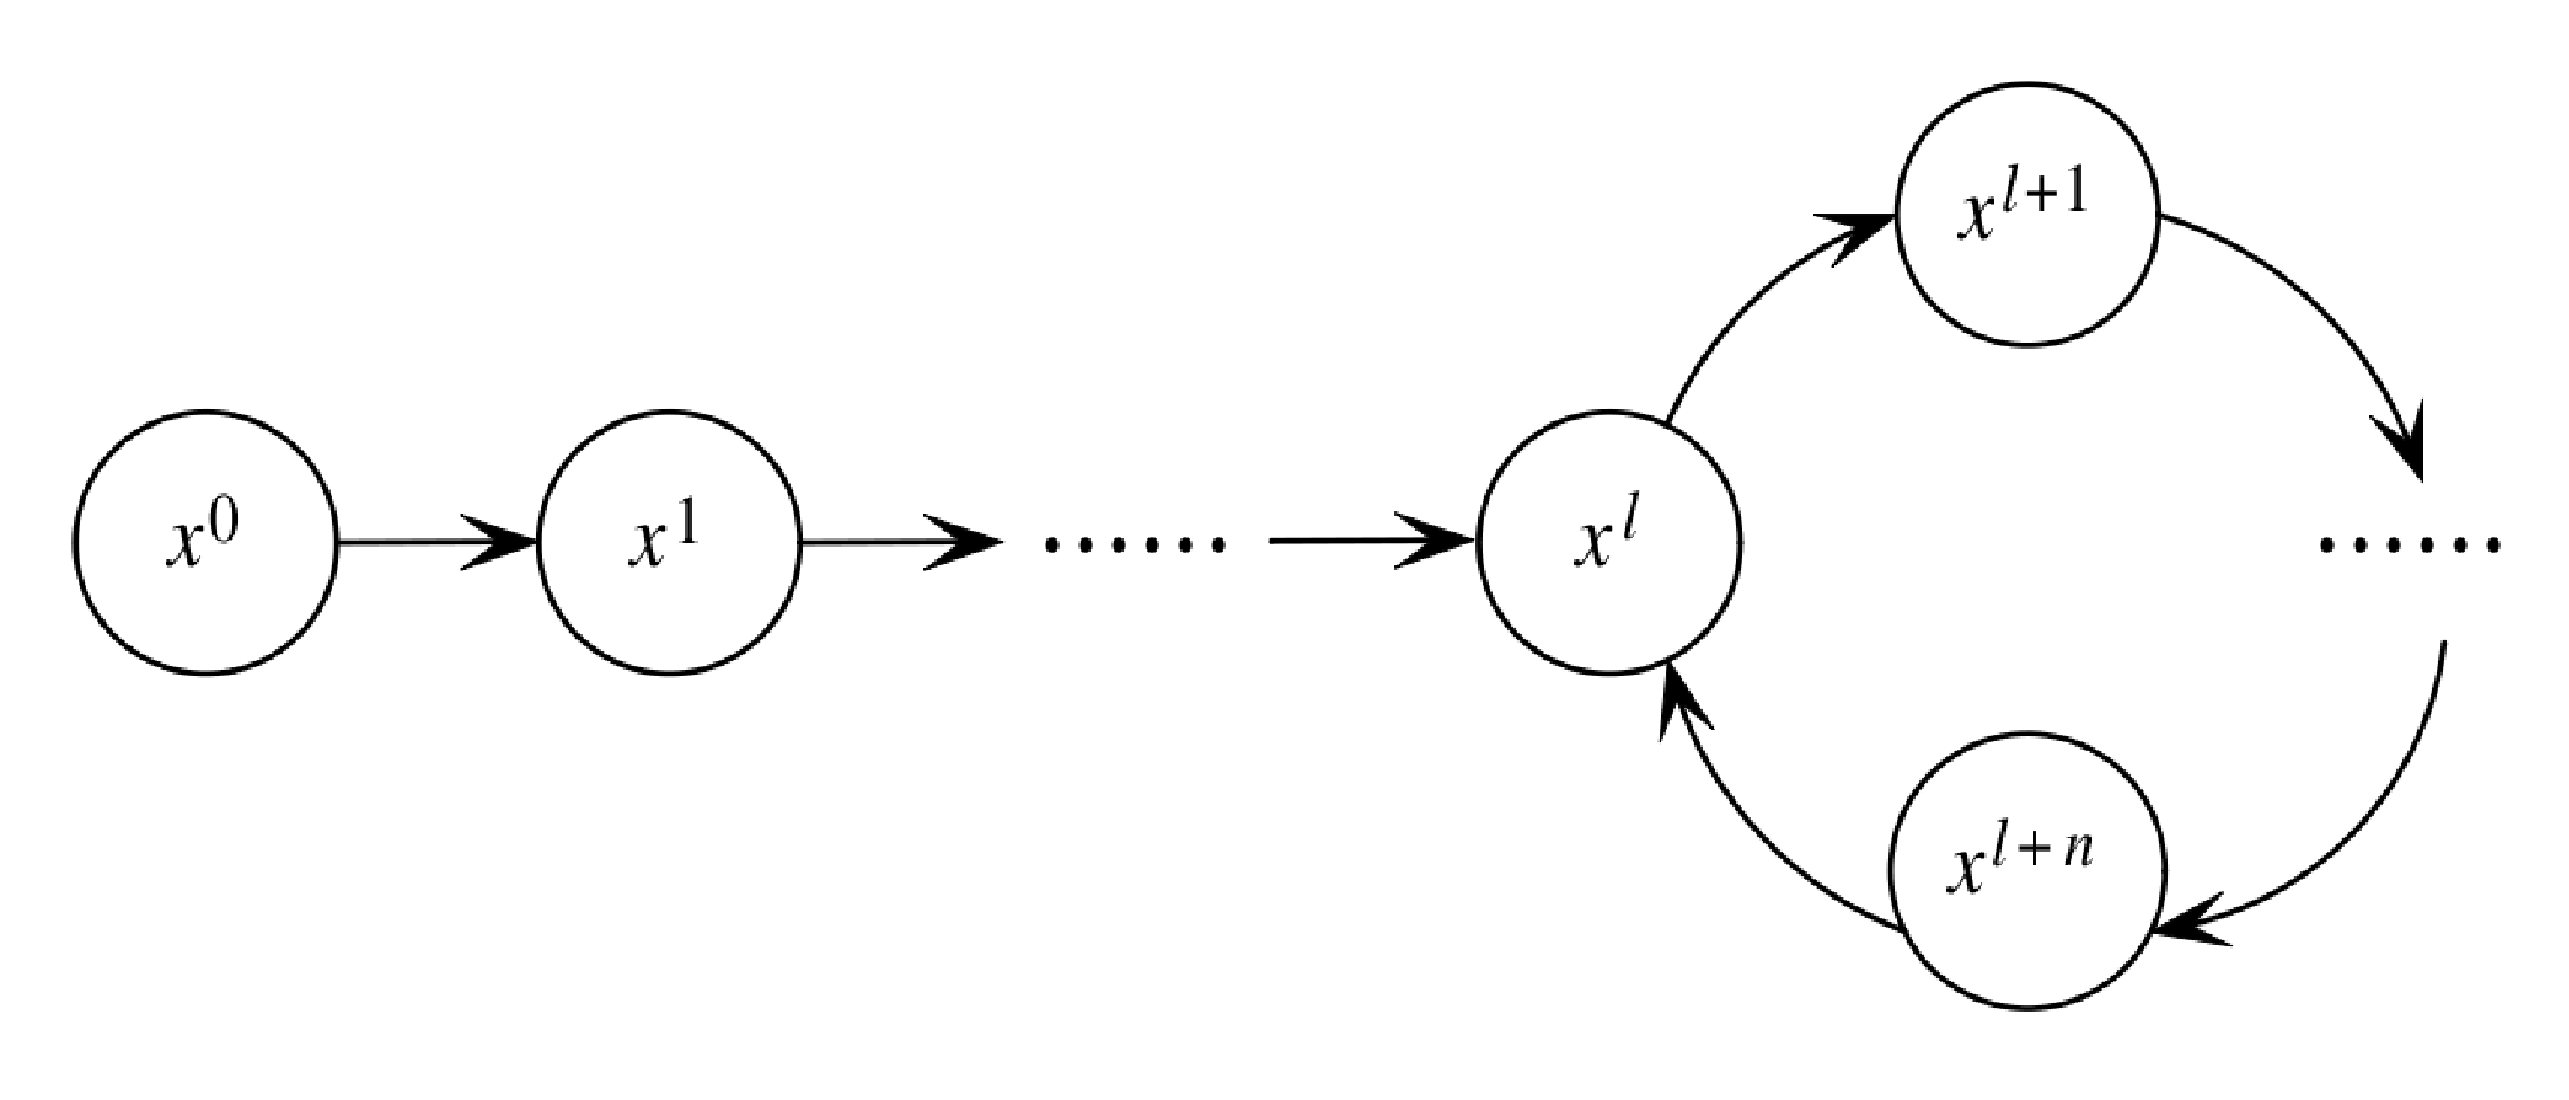
\includegraphics[scale=0.20]{pseudo_orbit.eps}
\caption{A pseudo orbit of a digital chaotic system}
\label{A pseudo orbit of a digital chaotic system}
\end{figure}


\begin{definition}%\cite{bahi102008}
A sequence $x = (x^{ 1} , ..., x^{n} )$ is said to be cyclic if a subset of successive terms is repeated from a given rank, until the end of $x$.
\end{definition}

This generator based on discrete chaotic iterations generated by two pseudorandom sequences ($m$ and $w$) has a long cycle length. If the cycle period of $m$ and $w$ are respectivelly $n_{m}$ and $n_{w}$, then in an ideal situation, the cycle period of the novel sequence is $n_{m} \times n_{w}\times 2$ (because $\bar{\bar{x}}=x$). Table \ref{The ideal cycle period} gives the ideal cycle period of various generators.

\begin{itemize}
\item $m$ ($n_{m}=2$): 12121212121212121212121212...

\item $w$ ($n_{w}=4$): 1 23 4 12 3 41 2 34 1 23 4 12 3 41 2 34 1 23 4...

\item $x$ ($n_{x}=2 \times 4 \times 2=16$): 0000(0) 1000(8) 1110(14) 1111(15) 0011(3) 0001(1) 1000(8) 1100(12) 1111(15) 0111(7) 0001(1) 0000(0) 1100(12) 1110(14) 0111(7) 0011(3) 0000(0) 1000(8) 1110(14) 1111(15) 0011(3) 0001(1) 1000(8) 1100(12) 1111(15) 0111(7) 0001(1) 0000(0) 1100(12) 1110(14) 0111(7) 0011(3)...

\end{itemize}


\begin{table}
\renewcommand{\arraystretch}{1.3}
\caption{Ideal cycle period}
\label{The ideal cycle period}
\centering
% \begin{tiny}
\begin{tabular}{|c|c|c|}\toprule\hline
\multicolumn{2}{|c|}{\textbf{PRNG}}&\textbf{Ideal cycle period}\\\hline
\multicolumn{2}{|c|}{\textbf{Logistic map}}& $\infty$\\\hline
\multicolumn{2}{|c|}{\textbf{XORshift}}&$2^{32}-1$ \\\hline
\multicolumn{2}{|c|}{\textbf{ISAAC}}& $2^{8295}$\\\hline
\multirow{4}*{\textbf{Version 1 CI algorithms}}&\textbf{Logistic map 1+Logistic map 2}&$\infty$\\\cline{2-3}
&\textbf{XORshift+XORshift}&$2^{65}$\\\cline{2-3}
&\textbf{XORshift+ISAAC}&$2^{8328}$\\\cline{2-3}
&\textbf{ISAAC+ISAAC}&$2^{16591}$\\\hline
\bottomrule
\end{tabular}
% \end{tiny}
\end{table}

\subsection{Security Analysis}
\label{Security Analysis Version 1 CI}
In this section the concatenation of two strings $u$ and $v$ is classically denoted by $uv$.
In a cryptographic context, a pseudo random generator is a deterministic algorithm $G$ transforming 
strings into strings and such that, for any seed 
$s$ of length m, $G(s)$ (the output of $G$ on the input $s$) has size $l_G(m)$ with $l_G(m) > m$. The notion of secure 
PRNGs can now be defined as follows.
\subsubsection{Algorithm expression conversion}
For the convenience of security analysis, Version 1 CI Algorithm \ref{Chaotic iteration} is converted as 
Equation~\ref{Version 1 CI Eq}, internal state is $x$, $S$ and $T$ are those computed by PRNG1 and PRNG2, 
each round, $x^{n-1}$ is updated to be $x^n$. 

\begin{equation}
\left\{
\begin{array}{l}
x^0 \in \llbracket 0, 2^\mathsf{N}-1 \rrbracket, S \in \llbracket 0, 2^\mathsf{N}-1 \rrbracket^\mathds{N}, T \in \llbracket 0, 2^\mathsf{N}-1 \rrbracket^\mathds{N}\\
C = S^n \& 1 + 3*N\\
w^0 = {T}^m~mod~N, w^1 = {T}^{m+1} \& 3, ... w^{C-1} = {T}^{m+C-1} \& 3\\ 
d^n = (1 \ll w^0) \oplus (1\ll w^1) \oplus ... (1 \ll w^{C-1})\\
\forall n \in \mathds{N}^*, x^n = x^{n-1} \oplus d^n,
\end{array}
\right.
\label{Version 1 CI Eq}
\end{equation}


\subsubsection{Proof}
\begin{definition}
\label{CSPRNG}
A cryptographic PRNG $G$ is secure if for any probabilistic polynomial time algorithm D, for any positive polynomial p, 
and for all sufficiently large m's,  
\begin{equation}
|Pr[D(G(U_m))=1]-Pr[D(U_{l_G(m)})=1]<\frac{1}{p(m)},
\end{equation}
where $U_r$ is the uniform distribution over ${0, 1}^r$ and the probabilities are taken over $U_m$, 
$U_{l_G(m)}$ as well as over the internal coin tosses of $D$.
\end{definition}

Intuitively, it means that there is no polynomial time algorithm that can distinguish a perfect uniform 
random generator from $G$ with a non negligible probability. Note that it is quite easily possible to change 
the function $l$ into any polynomial function $l'$ satisfying $l'(m)>m$.

The generation schema developed in Algorithm~\ref{Version 1 CI Eq} is based on $2$ pseudo random generators. Let $H$ 
be the ``PRNG1'' and $I$ be the ``PRNG2''. 
We may assume, without loss of generality, that for any string $S_0$ of size $L$,
the size of $H(S_0)$ is $kL$,  then for any string $T_0$ of size $M$, it has $I(T_0)$ with $kN$, with $k > 2$. 
It means that $l_H(N) = kL$ and $l_I(N) = kM$. Let $S_1,...,S_k$ be the string of length $L$ such that 
$H(S_0) = S_1 ... S_k$ and $T_1,...,T_k$ be the string of length
$M$ that $H(S_0) = T_1 ... T_k$ ($H(S_0)$ and $I(T_0)$ are the concatenations of $S_i$'s and $T_i$'s).
The cryptographic PRNG $X$ defined in Algorithm~\ref{Version 1 CI Eq} is algorithm mapping any string of length 
$L+M+N~ x_0S_0T_0$ into the string $x_0 \oplus d^1, 
x_0 \oplus d^1 \oplus d^2,... 
(x_0 \bigoplus^{i=k}_{i=0}d^i)$ (Equation~\ref{Version 1 CI Eq}).
One in particular has $l_X(L+M+N) = kN = l_H(N)$ and $k > M+L+N$.
We announce that if one PRNG of $H$ is secure, then the new one from Equation \ref{Version 1 CI Eq} 
is secure too.

\begin{proposition}
\label{cryptopreuve}
If one of $H$ is a secure cryptographic PRNG, then $X$ is a secure cryptographic
PRNG too.
\end{proposition}

\begin{proof}
The proposition is proven by contraposition. Assume that $X$ is not
secure. By Definition, there exists a polynomial time probabilistic
algorithm $D$, a positive polynomial $p$, such that for all $k_0$ there exists
$L+M+N\geq {k_0}$ satisfying 
$$| \mathrm{Pr}[D(X(U_{L+M+N}))=1]-\mathrm{Pr}[D(U_{kN}=1]|\geq \frac{1}{p(L+M+N)}.$$

Define there is a $w$ of size $kL$.
\begin{enumerate}
 \item Decompose $w$ into $w = w_1...w_k$.
 \item Pick a string $y$ of size $N$ uniformly at random.
 \item Pick a string of size $(3kN + \sum_{j=1}^{j=k}(w_j\&1)) M$: $u$.
 \item Decompose $u$ into $u = u_1...u_{3kN + \sum_{j=1}^{j=k}(w_j\&1)}$.
 \item Define $t_i = (\bigoplus_{l=3N(i-1)+(\sum_{l=1}^{l=i-1}(w_j\&1))+1}^
 {j=3N(i)+(\sum_{j=1}^{j=i}(w_j\&1))}(1<<u_l))$.
 \item Compute $z = (y\oplus t_1) (y\oplus t_1 \oplus t_2) ... (y\bigoplus_{i=1}^{i=k}(t_i))$.
 \item Return $D(z)$.
\end{enumerate}


On one hand, consider for each $y\in \mathbb{B}^{kN}$ the function $\varphi_{y}$
from $\mathbb{B}^{kN}$ into $\mathbb{B}^{kN}$ mapping $t=t_1\ldots t_k$
(each $t_i$ has length $N$) to 
$(y\oplus t_1 )(y\oplus t_1\oplus t_2)\ldots (y
  \bigoplus_{i=1}^{i=k} t_i)$. 
 On the other hand, treat each $u_l \in \mathbb{B}^{(3Nk + \sum_{j=0}^{j=k}(w_j\&1)) M}$ the function $\phi_{u}$
 from $\mathbb{B}^{(3kN + \sum_{j=0}^{j=k}(w_i\&1)) M}$ into $mathbb{B}^{kN}$ mapping $w = w_1 \ldots w_k$ (each 
 $w_i$ has length $L$) to 
 $(\bigoplus_{l=1}^{l=3N+(w_1\&1)}(1<<u_l)) ((\bigoplus_{l=1+3N+(w_1\&1)}^{l=6N+(w_1\&1)+(w_1\&1)}(1<<u_l)) \ldots 
 (\bigoplus_{l=3N(k-1)+\sum_{j=1}^{j=k-1}(w_j\&1)}^{l=3Nk+\sum_{j=1}^{j=k}(w_j\&1)}(1<<u_l)$
 By construction, one has for every $w$,
  
\begin{equation}\label{PCH-1}
D^\prime(w)=D(\varphi_y(\phi_u(w))),
\end{equation}

Therefore, and using (\ref{PCH-1}),
one has
$\mathrm{Pr}[D^\prime(U_{kL})=1]=\mathrm{Pr}[D(\varphi_y(\phi_u(U_{kL})))=1]$ and,
therefore, 
\begin{equation}\label{PCH-2}
\mathrm{Pr}[D^\prime(U_{kL})=1]=\mathrm{Pr}[D(U_{kN})=1].
\end{equation}

Now, using (\ref{PCH-1}) again, one has  for every $x$,
\begin{equation}\label{PCH-3}
\mathrm{Pr}[D^\prime(U_{H(x)})=1]=\mathrm{Pr}[D(\varphi_y(\phi_u(U_{H(x)})))=1] 
\end{equation}

since where $y$ and $u_j$ are randomly generated. \\
By construction, $\varphi_y(\phi_u(x))=X(yu_1w)$, hence 

\begin{equation}\label{PCH-4}
\mathrm{Pr}[D^\prime(H(U_{kL}))=1]=\mathrm{Pr}[D(X(U_{N+M+L}))=1]
\end{equation}

Compute the difference of Equation (\ref{PCH-4}) and (\ref{PCH-3}), one can deduce that
there exists a polynomial time probabilistic
algorithm $D^\prime$, a positive polynomial $p$, such that for all $k_0$ there exists
$L+M+N\geq {k_0}$ satisfying 
$$| \mathrm{Pr}[D^\prime(H(U_{KL}))=1]-\mathrm{Pr}[D(U_{kL})=1]|\geq \frac{1}{p(L+M+N)},$$
proving that $H$ is not secure, which is a contradiction to the first place that one 
of them is cryptographic secure. 
\end{proof}

\subsection{An Efficient, Cryptographically Secure, PRNG Based On Version 1 CI}
In Table~\ref{Version 1 CI cs}, an efficient, based on Version 1 CI, good random quality, and cryptographically secure 
PRNG algorithm is given.

\begin{table}
\centering
\begin{tabular}{|l|l|}
\hline
~\textbf{Input}: $x$ (a 12-bit word)\\
\hline
~\textbf{Output}: $r$ (a 12-bit word)\\
\hline
~$x1 \leftarrow xorshift1();$\\
~$x2 \leftarrow xorshift2();$\\
~$x3 \leftarrow xorshift3();$\\
~$t \leftarrow bbs();$\\
~$t1 \leftarrow t \& 1;$\\
~$t2 \leftarrow t \& 2;$\\
~$t3 \leftarrow t \& 4;$\\
~$w1 \leftarrow 0;$\\
~$w2 \leftarrow 0;$\\
~$w3 \leftarrow 0;$\\
~$\textbf{While}~ i = 1 ... 12$ \\
~$w1 \leftarrow (w1 \oplus (1 \ll ((x1 \gg (i\times 2))\&3)));$\\
~$w2 \leftarrow (w2 \oplus (1 \ll ((x2 \gg (i\times 2))\&3)));$\\
~$w3 \leftarrow (w3 \oplus (1 \ll ((x3 \gg (i\times 2))\&3)));$\\
~$\textbf{EndWhile}$\\
~$\textbf{if}~(t1 \neq 0)~\textbf{then}~w1 \leftarrow (w1 \oplus (1 \ll ((x1 \gg 26)\&3)));$ \\
~$\textbf{if}~(t2 \neq 0)~\textbf{then}~w2 \leftarrow (w2 \oplus (1 \ll ((x2 \gg 26)\&3)));$ \\
~$\textbf{if}~(t3 \neq 0)~\textbf{then}~w3 \leftarrow (w3 \oplus (1 \ll ((x3 \gg 26)\&3)));$ \\
~$x \leftarrow x \oplus w1 \oplus (w2 \ll 4) \oplus (w3 \ll 8);$\\
~$r \leftarrow x;$\\
~$\textbf{return} ~r;$\\
\hline
~\textbf{An arbitrary round of the algorithm}~\\
\hline
\end{tabular}
\caption{An Efficient, Cryptographically Secure, PRNG Based On Version 1 CI}
\label{Version 1 CI cs}
\end{table}

The internal state $x$ is defined as size of $12$ bits, three $32$-bit
XORshift PRNGs ($xorshift1(), xorshift2(), xorshift3()$) are applied, 
each of them is split to $16$ $2$-bit binary blocks (value is between 
$0$ to $3$), then the $3$ LSBs (least significant bits) of the output 
from BBS $bbs()$ are decide $12$ or $13$ these blocks used to update the 
state. According to Section~\ref{Security Analysis Version 1 CI}, this 
generator based on Version 1 CI can turn to be cryptographically secure if 
its $I$ used is cryptographically secure, here $I$ is chosen as BBS PRNG, 
which is believed to be the most secure PRNG method available~\cite{vmd}, 
the $t$ computed by BBS $bbs()$ is based on $32$ bit $m$ (Equation~\ref
{BBS Eq}), the $log(log(m))$ LSBs of $t$ can be treated as secure, hence, 
here $3$LSBs chosen is qualified.

\section{Version 2 CIPRNG Algorithm}
\subsection{Presentation}
The CI generator (generator based on chaotic iterations) is designed by the following process.
First of all, some chaotic iterations have to be done to generate a sequence 
$\left(x^n\right)_{n\in\mathds{N}} \in \left(\mathds{B}^\mathsf{N}\right)^\mathds{N}$ 
($\mathsf{N} \in \mathds{N}^*, \mathsf{N} \geqslant 2$, $N$ is not necessarily equal to 32) 
of boolean vectors, which are the successive states of the iterated system. Some of these vectors 
will be randomly extracted and our pseudo-random bit flow will be constituted by their components. 
Such chaotic iterations are realized as follows. 
Initial state $x^0 \in \mathds{B}^\mathsf{N}$ is a boolean vector taken as a 
seed (see Section~\ref{algo seed}) and chaotic strategy $\left(S^n\right)_{n\in\mathds{N}}\in 
\llbracket 1, \mathsf{N} \rrbracket^\mathds{N}$ is
an irregular decimation of a random number sequence (Section~\ref{Chaotic strategy}). The iterate function $f$ is
the vectorial boolean negation:
$$f_0:(x_1,...,x_\mathsf{N}) \in \mathds{B}^\mathsf{N} \longmapsto 
(\overline{x_1},...,\overline{x_\mathsf{N}}) \in \mathds{B}^\mathsf{N}.$$
At each iteration, only the $S^i$-th component of state $x^n$ is updated, 
as follows: $x_i^n = x_i^{n-1}$ if $i \neq S^i$, else $x_i^n = \overline{x_i^{n-1}}$.
Finally, some $x^n$ are selected
by a sequence $m^n$ as the pseudo-random bit sequence of our generator.
$(m^n)_{n \in \mathds{N}} \in \mathcal{M}^\mathds{N}$ is computed from 
a PRNG, such as XORshift sequence $(y^n)_{n \in \mathds{N}} \in \llbracket 0, 
2^{32}-1 \rrbracket$ (see Section~\ref{algo m}). So, the
generator returns the following values:\newline
\begin{small}
Bits:$$x_1^{m_0}x_2^{m_0}x_3^{m_0}\hdots x_\mathsf{N}^{m_0}x_1^{m_0+m_1}x_2^{m_0+m_1}\hdots x_\mathsf{N}^{m_0+m_1} x_1^{m_0+m_1+m_2}\hdots$$
or States:$$x^{m_0}x^{m_0+m_1}x^{m_0+m_1+m_2}\hdots$$
\end{small}


\subsection{The seed}
\label{algo seed}
The unpredictability of random sequences is established using
a random seed that is obtained by a physical source like timings of keystrokes.
Without the seed, the attacker must not be able to make any predictions about
the output bits, even when all details of the generator are known~\cite{Turan2008}.

The initial state of the system $x^0$ and the first term $y^0$ of the input PRNG are seeded either by
the current time in seconds since the Epoch, or by a number that the user inputs.
Different ways are possible. For example, let us denote by $t$ the decimal part of the current
time. So $x^0$ can be $t \text{ (mod $2^N$)}$ written in binary digits and $y^0 = t$.

\subsection{Sequence $m$ of returned states}
\label{algo m}
The output of the sequence $(y^n)$ is uniform in $\llbracket 0, 2^{32}-1 \rrbracket$. However, we do not want the output of $(m^n)$ to be uniform in $\llbracket 0, N \rrbracket$, because in this case, the returns of our generator will not be uniform in $\llbracket 0, 2^{N}-1 \rrbracket$, as it is illustrated in the following example. Let us suppose that $x^0=(0,0,0)$. Then $m^0 \in \llbracket 0, 3 \rrbracket$.
\begin{itemize}
\item If $m^0=0$, then no bit will change between the first and the second output of our new CI PRNG. Thus $x^1 = (0,0,0)$.
\item If $m^0=1$, then exactly one bit will change, which leads to three possible values for $x^1$, namely $(1,0,0)$, $(0,1,0)$, and $(0,0,1)$.
\item \emph{etc.}
\end{itemize}
As each value in $\llbracket 0, 2^3-1 \rrbracket$ must be returned with the same probability, then the values $(0,0,0)$, $(1,0,0)$, $(0,1,0)$, and $(0,0,1)$ must occur for $x^1$ with the same probability. Finally we see that, in this example, $m^0=1$ must be three times probable as $m^0=0$.
This leads to the following general definition for the probability of $m=i$:
\begin{equation}
P(m^n=i)=\frac{C^i_N}{2^N}
\end{equation}

Then, here is an example for the $(m^n)$ sequence with a selector function $g_1$
\begin{equation}
\label{v2_g1}
m^n = g_1(y^n)=
\left\{
\begin{array}{l}
0 \text{ if }0 \leqslant\frac{y^n}{2^{32}}<\frac{C^0_N}{2^N},\\
1 \text{ if }\frac{C^0_N}{2^N} \leqslant\frac{y^n}{2^{32}}<\sum_{i=0}^1\frac{C^i_N}{2^N},\\
2 \text{ if }\sum_{i=0}^1\frac{C^i_N}{2^N} \leqslant\frac{y^n}{2^{32}}<\sum_{i=0}^2\frac{C^i_N}{2^N},\\
\vdots~~~~~ ~~\vdots~~~ ~~~~\\
N \text{ if }\sum_{i=0}^{N-1}\frac{C^i_N}{2^N} \leqslant\frac{y^n}{2^{32}}<1.\\
\end{array}
\right.
\end{equation}

Let us notice, to conclude this subsection, that our new CI PRNG can use any reasonable function as selector. 
In this paper, $g_1()$ and $g_2()$ are adopted for demonstration purposes, where:
\begin{equation}
\label{v2_g2}
m^n = g_2(y^n)=
\left\{
\begin{array}{l}
N \text{ if }0 \leqslant\frac{y^n}{2^{32}}<\frac{C^0_N}{2^N},\\
N-1 \text{ if }\frac{C^0_N}{2^N} \leqslant\frac{y^n}{2^{32}}<\sum_{i=0}^1\frac{C^i_N}{2^N},\\
N-2 \text{ if }\sum_{i=0}^1\frac{C^i_N}{2^N} \leqslant\frac{y^n}{2^{32}}<\sum_{i=0}^2\frac{C^i_N}{2^N},\\
\vdots~~~~~ ~~\vdots~~~ ~~~~\\
0 \text{ if }\sum_{i=0}^{N-1}\frac{C^i_N}{2^N} \leqslant\frac{y^n}{2^{32}}<1.\\
\end{array}
\right.
\end{equation}

In this thesis, $g_1()$ is the selector function unless noted otherwise. And we will show later that both of $g_1()$ and $g_2()$ can pass all of the performed tests. 

\begin{figure}
\centering
\subfigure [The histogram of adjacent output distribution $m^n = g_1(y^n)$]{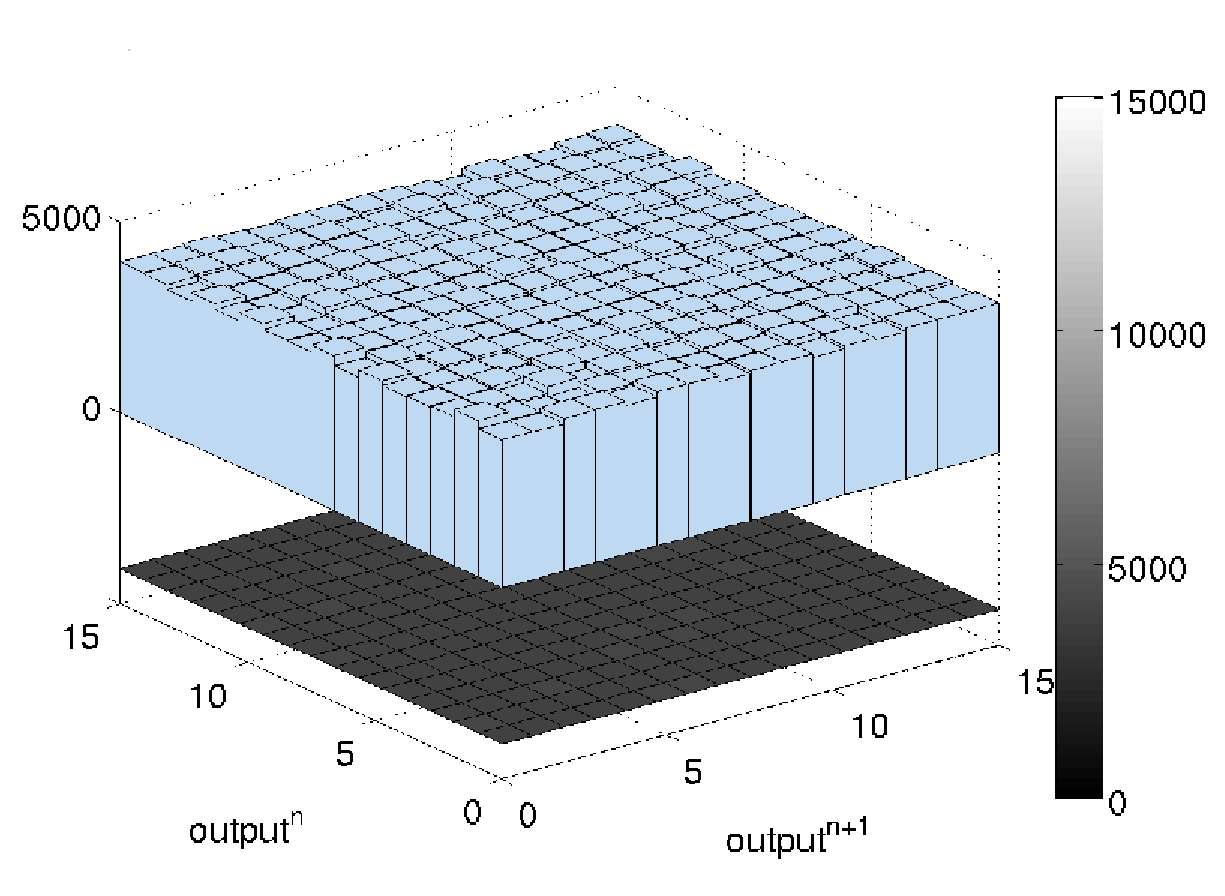
\includegraphics[scale=0.4]{fy.eps}
\label{Histogram1}} \hspace{0.4cm}
\subfigure [The histogram of adjacent output distribution $m^n = g_2(y^n)$]{\includegraphics[scale=0.3]{f2y.eps}
\label{Histogram2}} \hspace{0.4cm}
\subfigure [The histogram of adjacent output distribution $m^n = y^n ~ mod ~ 4$]{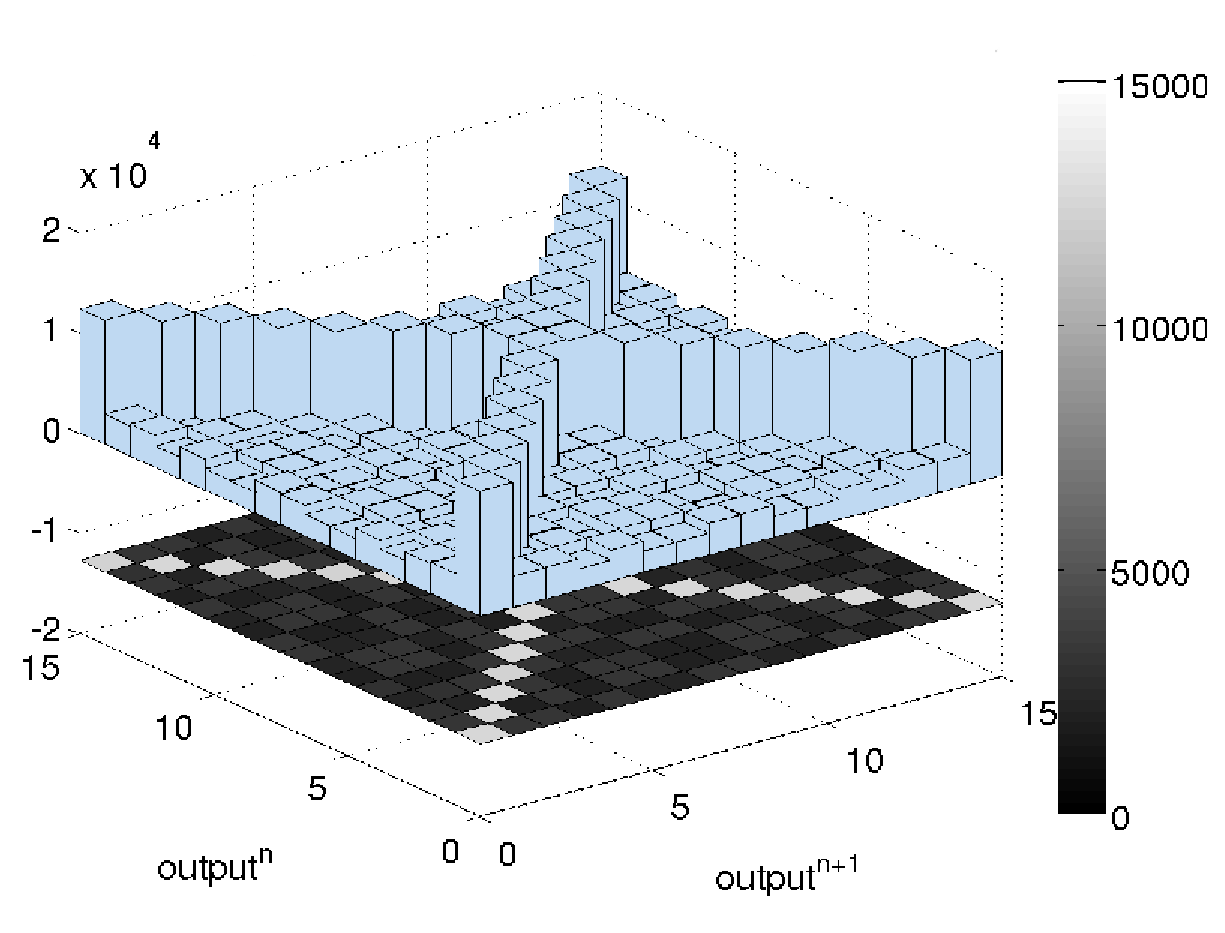
\includegraphics[scale=0.4]{y.eps}%
\label{Histogram3}} \hspace{0.4cm}
\caption{Histogram and intensity maps}
\label{Histogram and intensity map1}
\end{figure}

In order to evaluate our proposed method and compare its statistical properties with various other methods, the density histogram and intensity map of adjacent output have been computed. The length of $x$ is $N = 4$ bits, and the initial conditions and control
parameters are the same. A large number of
sampled values are simulated ($10^6$ samples). 
Figure~\ref{Histogram1} and Figure~\ref{Histogram2} shows the intensity map for $m^n=g_1(y^n)$ and $m^n=g_2(y^n)$.
In order to appear random, the histogram should be uniformly distributed in all areas. 
It can be observed that uniform histograms and flat color intensity maps are obtained when using our schemes. 
Another illustration of this fact is given by Figure~\ref{Histogram3}, whereas its uniformity is further justified by the tests presented in Section \ref{Test for Version 2 CI}.


\subsection{Chaotic strategy}
\label{Chaotic strategy}
The chaotic strategy $(S^k) \in \llbracket 1, N \rrbracket^\mathds{N}$ is generated from a second XORshift sequence $(b^k) \in \llbracket 1, N \rrbracket^\mathds{N}$. The only difference between the sequences $S$ and $b$ is that some terms of $b$ are discarded, in such a way that $\forall k \in \mathds{N}, (S^{M^k}, S^{M^k+1}, \hdots, S^{M^{k+1}-1})$ does not contain any given integer twice, where $M^k = \sum_{i=0}^k m^i$. Therefore, no bit will change more than once between two successive outputs of our PRNG, increasing the speed of the former generator by doing so. $S$ is said to be ``an irregular decimation'' of $b$. This decimation can be obtained by the following process.

Let $(d^1,d^2,\dots,d^N)\in \{0,1\}^N$ be a mark sequence, such that whenever $\sum_{i=1}^N d^i = m^k$,
then $\forall i, d_i=0$ ($\forall k$, the sequence is reset when $d$ contains $m^k$ times the number 1). This mark sequence will control the XORshift sequence $b$ as follows:
\begin{itemize}
\item if $d^{b^j} \neq 1$, then $S^k=b^j$, $d^{b^j} = 1$, and $k = k+1$,
\item if $d^{b^j}=1$, then $b^j$ is discarded.
\end{itemize}
For example, if $b = 142\underline{2}334 1421\underline{1}\underline{2}\underline{2}34...$ and $m = 4341...$, then $S=1423~341~4123~4...$ However, if we do not use the mark sequence, then one position may change more than once and the balance property will not be checked, due to the fact that $\bar{\bar{x}}=x$. As an example, for $b$ and $m$ as in the previous example, $S=1422~334~1421~1...$ and $S=14~4~42~1...$ lead to the same output (because switching the same bit twice leads to the same state).

 
To check the balance property, a set of 500
sequences are generated with and without decimation, each
sequence containing $10^6$ bits. Figure~\ref{nmark} shows the
percentages of differences between zeros and ones, and presents a better balance property for the sequences with decimation. This claim will be verified in the tests section (Section \ref{Results of NISTfor new CI}). 


Another example is given in Table~\ref{table application example}, in which $r$ means ``reset'' and the integers which are underlined in sequence $b$ are discarded.





\begin{figure}
\centering
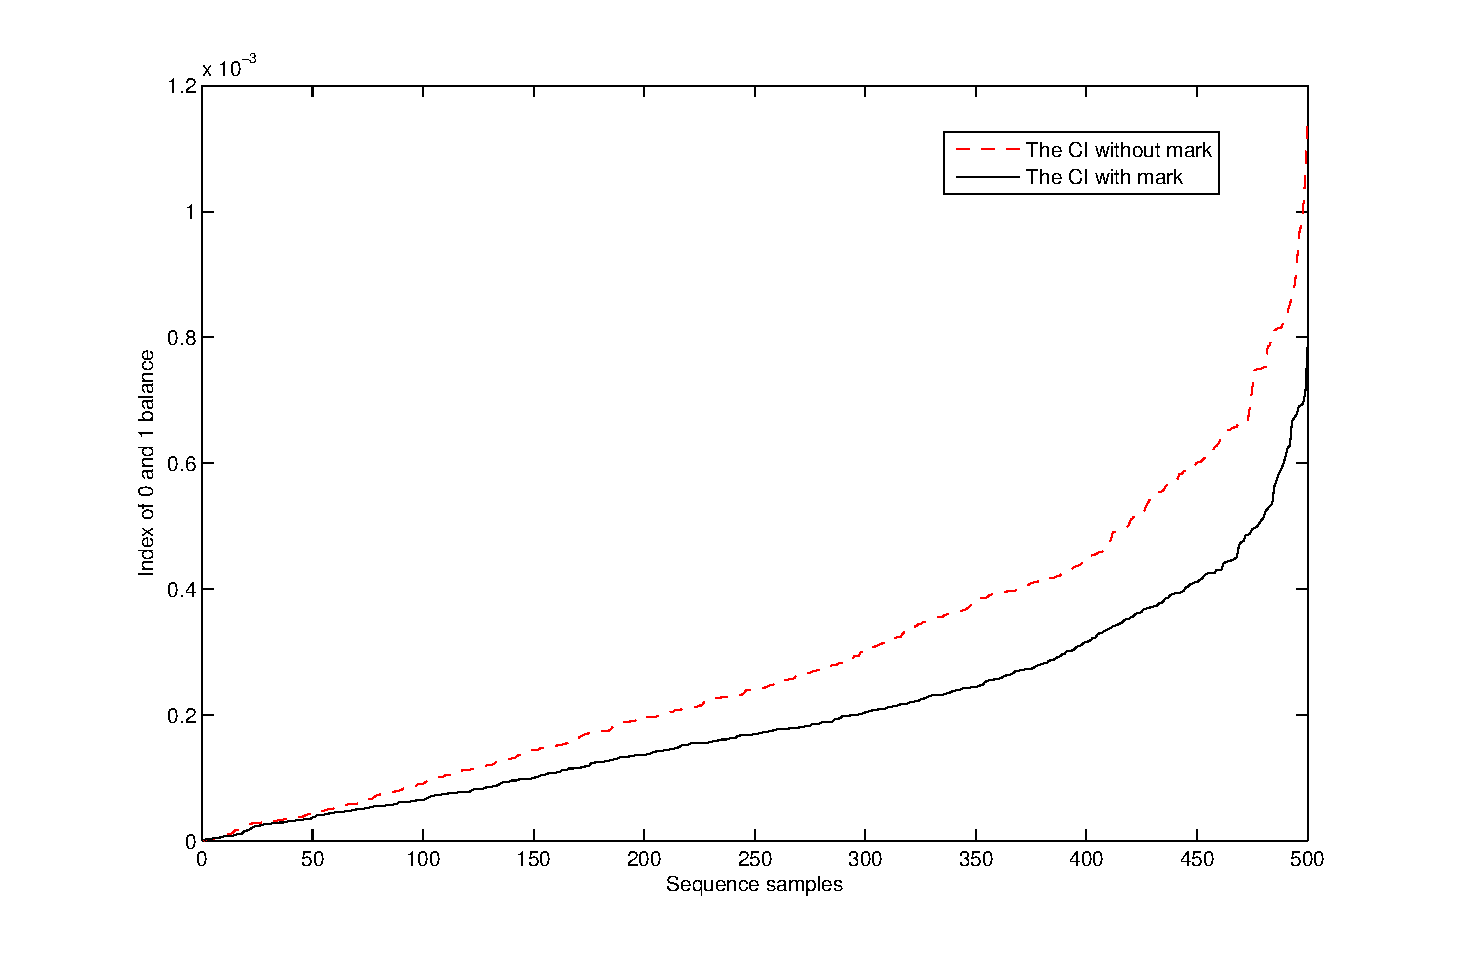
\includegraphics[width=3.85in]{nmark.eps}
\DeclareGraphicsExtensions.
\caption{Balance property}
\label{nmark}
\end{figure}

\subsection{Version 2 CI Algorithm}

The basic design procedure of the novel generator is summed up in Algorithm~\ref{Chaotic iteration1}.
The internal state is $x$, the output state is $r$. $a$ and $b$ are those computed by the two input
PRNGs. The value $g_1(a)$ is an integer, defined as in Equation~\ref{v2_g1}. Lastly, $\mathsf{N}$ is a constant 
defined by the user.
\begin{algorithm}
\textbf{Input:} the internal state $x$ ($\mathsf{N}$ bits)\\
\textbf{Output:} a state $r$ of $\mathsf{N}$ bits
\begin{algorithmic}[1]
\FOR{$i=0,\dots,N$}
{
\STATE$d_i\leftarrow{0}$\;
}
\ENDFOR
\STATE$a\leftarrow{PRNG1()}$\;
\STATE$m\leftarrow{f(a)}$\;
\STATE$k\leftarrow{m}$\;
\WHILE{$i=0,\dots,k$}

\STATE$b\leftarrow{PRNG2()~mod~\mathsf{N}}$\;
\STATE$S\leftarrow{b}$\;
    \IF{$d_S=0$}
    {
\STATE      $x_S\leftarrow{ \overline{x_S}}$\;
\STATE      $d_S\leftarrow{1}$\;
    
    }
    \ELSIF{$d_S=1$}
    {
\STATE      $k\leftarrow{ k+1}$\;
    }\ENDIF
\ENDWHILE
$r\leftarrow{x}$\;
return $r$\;
\medskip
\caption{An arbitrary round of the Version 2 CI generator}
\label{Chaotic iteration1}
\end{algorithmic}
\end{algorithm}


As a comparison, the basic design procedure of the old generator 
is recalled in Algorithm~\ref{Chaotic iteration2} ($a$ and $b$ are computed by two input PRNGs, 
$\mathsf{N}$ and $c\geqslant 3\mathsf{N}$ are constants defined by the user). 
See Subsection~\ref{Version 1 CI algorithms and examples} for further information.


\begin{algorithm}
\textbf{Input:} the internal state $x$ (an array of $\mathsf{N}$ 1-bit words)\\
\textbf{Output:} an array $r$ of $\mathsf{N}$ 1-bit words
\begin{algorithmic}[1]

\STATE$a\leftarrow{PRNG1()}$;
\STATE$m\leftarrow{a~mod~2+c}$;
\WHILE{$i=0,\dots,m$}
\STATE$b\leftarrow{PRNG2()}$;
\STATE$S\leftarrow{b~mod~\mathsf{N}}$;
\STATE$x_S\leftarrow{ \overline{x_S}}$;
\ENDWHILE
\STATE$r\leftarrow{x}$;
\STATE return $r$;
\medskip
\caption{An arbitrary round of the old CI generator}
\label{Chaotic iteration2}
\end{algorithmic}
\end{algorithm}


\subsection{Illustrative Example of Version 2 CI (XORshift, XORshift)}

In this example, $\mathsf{N} = 4$ is chosen for easy understanding and the input PRNG is XORshift PRNG.
As stated before, the initial state of the system $x^0$ can be seeded by the decimal part $t$ of the current time.
For example, if the current time in seconds since the Epoch is 1237632934.484088,
so $t = 484088$, then $x^0 = t \text{ ($mod$ 16)}$ in binary digits, \emph{i.e.}, $x^0 = ( 0, 1, 0, 0)$.

To compute $m$ sequence, Equation~\ref{v2_g1} can be adapted to this example as follows:
\begin{equation}
\label{m1 fuction}
m^n=g_1(y^n)=
\left\{
\begin{array}{llccccc}
0 & \text{ if }&0 &\leqslant&\frac{y^n}{2^{32}}&<&\frac{1}{16},\\
1 & \text{ if }&\frac{1}{16} &\leqslant&\frac{y^n}{2^{32}}&<&\frac{5}{16} ,\\
2 & \text{ if }&\frac{5}{16} &\leqslant&\frac{y^n}{2^{32}}&<&\frac{11}{16},\\
3 & \text{ if }&\frac{11}{16} &\leqslant&\frac{y^n}{2^{32}}&<&\frac{15}{16},\\
4 & \text{ if }&\frac{15}{16} &\leqslant&\frac{y^n}{2^{32}}&<&1,\\
\end{array}
\right.
\end{equation}

\noindent where $y$ is generated by XORshift seeded with the current time. 
We can see that the probabilities of occurrences of $m=0$, $m=1$, $m=2$, $m=3$, $m=4$, 
are $\frac{1}{16}$, $\frac{4}{16}$, $\frac{6}{16}$, $\frac{4}{16}$, $\frac{1}{16}$, respectively. 
This $m$ determines what will be the next output $x$. For instance,
\begin{itemize}
\item If $m=0$, the following $x$ will be $( 0, 1, 0, 0)$.
\item If $m=1$, the following $x$ can be $( 1, 1, 0, 0)$, $( 0, 0, 0, 0)$, $( 0, 1, 1, 0)$, or $( 0, 1, 0, 1)$.
\item If $m=2$, the following $x$ can be $( 1, 0, 0, 0)$, $( 1, 1, 1, 0)$, $( 1, 1, 0, 1)$, $( 0, 0, 1, 0)$, $( 0, 0, 0, 1)$, or $( 0, 1, 1, 1)$.
\item If $m=3$, the following $x$ can be $( 0, 0, 1, 1)$, $( 1, 1, 1, 1)$, $( 1, 0, 0, 1)$, or $( 1, 0, 1, 0)$.
\item If $m=4$, the following $x$ will be $( 1, 0, 1, 1)$.
\end{itemize}

In this simulation, $m = 0, 4, 2, 2, 3, 4, 1, 1, 2, 3, 0, 1, 4,...$ Additionally, 
$b$ is computed with a XORshift generator too, but with another seed. We have found 
$b = 1, 4, 2, 2, 3, 3, 4, 1, 1, 4, 3, 2, 1,...$

Chaotic iterations are made with initial state $x^0$, vectorial logical negation $f_0$, and
strategy $S$. The result is presented in Table~\ref{table application example}. Let us 
recall that sequence $m$ gives the states $x^n$ to return, which are here $x^0, x^{0+4}, 
x^{0+4+2}, \hdots$ So, in this example, the output of the generator is: 10100111101111110011... or 4,4,11,8,1...




\begin{table*}[!t]
%\renewcommand{\arraystretch}{1.3}
\centering
\begin{tabular}{|c|c@{}c|c@{}c@{}c@{}c@{}c@{}c|c@{}c@{}c|c@{}c@{}c@{}c|}
\hline
$m$ &0 & &4 & & & & & &2& &&2&&  &  \\ \hline
$k$ &0 & &4 & & &$+1$ & & &2& &&2&$+1$&  &  \\ \hline
$b$  &  & &1 &4&2&\underline{2}       &3& &3&4&&1&\underline{1}      &4&\\ \hline
$d$  &r  & &r~$\left(\begin{array}{c}1\\0\\0\\0\end{array}\right)$ & $\left(\begin{array}{c}1\\0\\0\\1\end{array}\right)$ & $\left(\begin{array}{c}1\\1\\0\\1\end{array}\right)$ & & $\left(\begin{array}{c}1\\1\\1\\1\end{array}\right)$ && r~$\left(\begin{array}{c}0\\0\\1\\0\end{array}\right)$ &$\left(\begin{array}{c}0\\0\\1\\1\end{array}\right)$ &&r~$\left(\begin{array}{c}1\\0\\0\\0\end{array}\right)$ & &$\left(\begin{array}{c}1\\0\\0\\1\end{array}\right)$  &  \\ \hline
$S$  &  & &1 &4&2&        &3& &3&4&&1& &4 &  \\ \hline
$x^{0}$ &  &$x^{0}$ & & &  
&  & &$x^{4}$ & & &   
$x^{6}$& & &&$x^{8}$  \\
%1ere ligne
0 & &0 &$\xrightarrow{1} 1$ & &
 & &   &1   & & &
1 &$\xrightarrow{1} 0$ & & & 0\\
%2eme ligne
1 &  &1 &   &   &
$\xrightarrow{2} 0$ & & &0 & & &
0 & &  &&0\\
%3eme ligne
0 & &0 & & &
 & &$\xrightarrow{3} 1$ &1 &$\xrightarrow{3} 0$ & &
0 &   & & &0  \\
% 4eme ligne
0 & &0  & &$\xrightarrow{4} 1$ &
 & & &1 & &$\xrightarrow{4} 0$ &
0 & & &$\xrightarrow{4} 1$&1 \\
\hline
\end{tabular}\\
\vspace{0.5cm}
Binary Output: $x_1^{0}x_2^{0}x_3^{0}x_4^{0}x_1^{4}x_2^{4}x_3^{4}x_4^{4}x_1^{6}x_2^{6}... = 0100101110000001...$\\
Integer Output:
$x^{0},x^{4},x^{6},x^{8}... = 4,11,8,1...$
\caption{Example of New CI(XORshift,XORshift) generation}
\label{table application example}
\end{table*}

\subsection{Security Analysis}
\label{Security Analysis Version 2 CI}
In this section the concatenation of two strings $u$ and $v$ is classically denoted by $uv$.
In a cryptographic context, a pseudo random generator is a deterministic algorithm $G$ transforming 
strings into strings and such that, for any seed 
$s$ of length m, $G(s)$ (the output of $G$ on the input $s$) has size $l_G(m)$ with $l_G(m) > m$. The notion of secure 
PRNGs can now be defined as follows.
\subsubsection{Algorithm expression conversion}
For the convenience of security analysis, Version 2 CI Algorithm \ref{Chaotic iteration1} is converted as 
Equation~\ref{Version 2 CI Eq}, internal state is $x$, $S$ and $T$ are those computed by PRNG1 and PRNG2, 
each round, $x^{n-1}$ is updated to be $x^n$. 

\begin{equation}
\label{g}
m^n = g(S^n)=
\left\{
\begin{array}{l}
0 \text{ if }0 \leqslant{S^n}<{C^0_{32}},\\
1 \text{ if }{C^0_{32}} \leqslant{S^n}<\sum_{i=0}^1{C^i_{32}},\\
2 \text{ if }\sum_{i=0}^1{C^i_{32}} \leqslant{S^n}<\sum_{i=0}^2{C^i_{32}},\\
\vdots~~~~~ ~~\vdots~~~ ~~~~\\
N \text{ if }\sum_{i=0}^{N-1}{C^i_{32}}\leqslant{S^n}<1.\\
\end{array}
\right.
\end{equation}

\begin{algorithm}
\textbf{Input:} the internal state $d$, $m$, and PRNG sequence $T$\\
\textbf{output:} a state $r$\\
\begin{algorithmic}[1]
\WHILE{$i=0,\dots,m$}
\STATE$w^i\leftarrow{T^{l+i}}~mod~N$\;
    \IF{$d^n_{w^i}=0$}
    {
\STATE      $d^n_{w^i}\leftarrow{1}$\;

    }
    \ELSIF{$d^n_{w^i}=1$}
    {
\STATE      $k\leftarrow{ k+1}$\;
    }\ENDIF
\ENDWHILE
\STATE $r \leftarrow  d^n $\;
\medskip
\caption{Algorithm for $h(d,m,T)$}
\label{h}
\end{algorithmic}
\end{algorithm}

\begin{equation}
\left\{
\begin{array}{l}
x^0 \in \llbracket 0, 2^\mathsf{N}-1 \rrbracket, S \in \llbracket 0, 2^\mathsf{N}-1 \rrbracket^\mathds{N}, T \in \llbracket 0, 2^\mathsf{N}-1 \rrbracket^\mathds{N}\\
m = g(S^n)(Equation~\ref{g});\\
d^n = 0;\\
d^n = h(d^n,m,T)(Equation~\ref{h});\\
\forall n \in \mathds{N}^*, x^n = x^{n-1} \oplus d^n,
\end{array}
\right.
\label{Version 2 CI Eq}
\end{equation}

\subsubsection{Proof}
\begin{definition}
\label{CSPRNG}
A cryptographic PRNG $G$ is secure if for any probabilistic polynomial time algorithm D, for any positive polynomial p, 
and for all sufficiently large m's,  
\begin{equation}
|Pr[D(G(U_m))=1]-Pr[D(U_{l_G(m)})=1]<\frac{1}{p(m)},
\end{equation}
where $U_r$ is the uniform distribution over ${0, 1}^r$ and the probabilities are taken over $U_m$, 
$U_{l_G(m)}$ as well as over the internal coin tosses of $D$.
\end{definition}

Intuitively, it means that there is no polynomial time algorithm that can distinguish a perfect uniform 
random generator from $G$ with a non negligible probability. Note that it is quite easily possible to change 
the function $l$ into any polynomial function $l'$ satisfying $l'(m)>m$.

The generation schema developed in Algorithm~\ref{Chaotic iteration1} is based on $2$ pseudo random generators. Let $H$ 
be the ``PRNG1'' and $I$ be the ``PRNG2''. 
We may assume, without loss of generality, that for any string $S_0$ of size $L$,
the size of $H(S_0)$ is $kL$,  then for any string $T_0$ of size $M$, it has $I(T_0)$ with $kM$, with $k > 2$. 
It means that $l_H(L) = kL$ and $l_I(M) = kM$. Let $S_1,...,S_k$ be the string of length $L$ such that 
$H(S_0) = S_1 ... S_k$ and $T_1,...,T_k$ be the string of length
$M$ that $H(S_0) = T_1 ... T_k$ ($H(S_0)$ and $I(T_0)$ are the concatenations of $S_i$'s and $T_i$'s).
The cryptographic PRNG $X$ defined in Algorithm~\ref{Version 2 CI Eq} is algorithm mapping any string of length 
$N+M+L~ x_0S_0T_0$ into the string $x_0 \oplus d^1, 
x_0 \oplus d^1 \oplus d^2,... 
(x_0 \bigoplus^{i=k}_{i=0}d^i)$ (Equation~\ref{Version 2 CI Eq}).
One in particular has $l_X(L+M+N) = kN = l_H(N)$ and $k > M+L+N$.
We announce that if one PRNG of $H$ is secure, then the new one from Equation \ref{Version 1 CI Eq} 
is secure too.

\begin{proposition}
\label{cryptopreuve}
If one of $H$ is a secure cryptographic PRNG, then $X$ is a secure cryptographic
PRNG too.
\end{proposition}

\begin{proof}
The proposition is proven by contraposition. Assume that $X$ is not
secure. By Definition, there exists a polynomial time probabilistic
algorithm $D$, a positive polynomial $p$, such that for all $k_0$ there exists
$L+M+N\geq {k_0}$ satisfying 
$$| \mathrm{Pr}[D(X(U_{L+M+N}))=1]-\mathrm{Pr}[D(U_{kN}=1]|\geq \frac{1}{p(L+M+N)}.$$

Define there is a $w$ of size $kL$.
\begin{enumerate}
 \item Decompose $w$ into $w = w_1...w_k$.
 \item Define $m$ into $m_1 = w_1~mod~N, m_2 = w_2 ~mod~N, ... m_k = w_k~mod~N$.
 \item Pick a string $y$ of size $N$ uniformly at random.
 \item Pick a string $u = {u_1,u_2...u_k}$, which is satisfied with processing $k$ times $h(0, m, u)$.
 \item Define $t_i = h(0,m_i,u_i)$.
 \item Compute $z = (y\oplus t_1) (y\oplus t_1 \oplus t_2) ... (y\bigoplus_{i=1}^{i=k}(t_i))$.
 \item Return $D(z)$.
\end{enumerate}


On one hand, consider for each $y\in \mathbb{B}^{kN}$ the function $\varphi_{y}$
from $\mathbb{B}^{kN}$ into $\mathbb{B}^{kN}$ mapping $t=t_1\ldots t_k$
(each $t_i$ has length $N$) to 
$(y\oplus t_1 )(y\oplus t_1\oplus t_2)\ldots (y
  \bigoplus_{i=1}^{i=k} t_i)$. 
 On the other hand, treat each $u_l \in \mathbb{B}^{(3Nk + \sum_{j=0}^{j=k}(w_j\&1)) M}$ the function $\phi_{u}$
 from $\mathbb{B}^{(3kN + \sum_{j=0}^{j=k}(w_i\&1)) M}$ into $mathbb{B}^{kN}$ mapping $w = w_1 \ldots w_k$ (each 
 $w_i$ has length $L$) to 
 $(\bigoplus_{l=1}^{l=3N+(w_1\&1)}(1<<u_l)) ((\bigoplus_{l=1+3N+(w_1\&1)}^{l=6N+(w_1\&1)+(w_1\&1)}(1<<u_l)) \ldots 
 (\bigoplus_{l=3N(k-1)+\sum_{j=1}^{j=k-1}(w_j\&1)}^{l=3Nk+\sum_{j=1}^{j=k}(w_j\&1)}(1<<u_l)$
 By construction, one has for every $w$,
  
\begin{equation}\label{PCH-11}
D^\prime(w)=D(\varphi_y(\phi_u(w))),
\end{equation}

Therefore, and using (\ref{PCH-11}),
one has
$\mathrm{Pr}[D^\prime(U_{kL})=1]=\mathrm{Pr}[D(\varphi_y(\phi_u(U_{kL})))=1]$ and,
therefore, 
\begin{equation}\label{PCH-22}
\mathrm{Pr}[D^\prime(U_{kL})=1]=\mathrm{Pr}[D(U_{kN})=1].
\end{equation}

Now, using (\ref{PCH-11}) again, one has  for every $x$,
\begin{equation}\label{PCH-33}
\mathrm{Pr}[D^\prime(U_{H(x)})=1]=\mathrm{Pr}[D(\varphi_y(\phi_u(U_{H(x)})))=1] 
\end{equation}

since where $y$ and $u_j$ are randomly generated. \\
By construction, $\varphi_y(\phi_u(x))=X(yu_1w)$, hence 

\begin{equation}\label{PCH-44}
\mathrm{Pr}[D^\prime(H(U_{kL}))=1]=\mathrm{Pr}[D(X(U_{N+M+L}))=1]
\end{equation}

Compute the difference of Equation (\ref{PCH-44}) and (\ref{PCH-33}), one can deduce that
there exists a polynomial time probabilistic
algorithm $D^\prime$, a positive polynomial $p$, such that for all $k_0$ there exists
$L+M+N\geq {k_0}$ satisfying 
$$| \mathrm{Pr}[D^\prime(H(U_{KL}))=1]-\mathrm{Pr}[D(U_{kL})=1]|\geq \frac{1}{p(L+M+N)},$$
proving that $H$ is not secure, which is a contradiction to the first place that one 
of them is cryptographic secure. 
\end{proof}



\section{Version 3 LUT CI(XORshift,XORshift) algorithms}
\label{LUT CI(XORshift,XORshift) algorithms and example}
\subsection{Introduction}

The LUT (Lookup-Table) CI generator is an improved version of the new CI generator. The key-ideas are:
\begin{itemize}
\item To use a Lookup Table for a faster generation of strategies. 
These strategies satisfy the same property than the ones provided by the decimation process.
\item And to use all the bits provided by the two inputted generators (to discard none of them).
\end{itemize}
%Before putting these key-ideas together, we can make a first practical remark in order to improve the speed of all of our generators.
These key-ideas are put together by the following way.

%In the LUT version of the proposed generator, chaotic iterations are realized as in the new CI PRNG, in order to generate a sequence $\left(x^n\right)_{n\in\mathds{N}} \in \left(\mathds{B}^N\right)^\mathds{N}$ of Boolean vectors ($N \in \mathds{N}^*, N \geqslant 2$).
Let us firstly recall that in chaotic iterations, only the cells designed by $S^{n}-$th are ``iterated'' 
at the $n^{th}$ iteration.
$S^n$ can be either a component (\emph{i.e.}, only one cell is updated at each iteration, 
so $S^n \in \llbracket 1;N \rrbracket$) or a subset of components (any number of cells can be 
updated at each iteration, that is, $S^n \subset \llbracket 1;N \rrbracket$).
The first kind of strategies are called ``unary strategies'' whereas the second one are denoted by ``general strategies''.
In the last case, each term $S^n$ of the strategy can be represented by an integer lower than $2^N$, 
designed by $\mathcal{S}^n$, for a system having $N$ bits: the $k^{th}$ component of the system is 
updated at iteration number $n$ if and only if the $k^{th}$ digit of the binary decomposition of $\mathcal{S}^n$ is 1.
For instance, let us consider that $\mathcal{S}^n=5$, and that we iterate on a system having 6 bits ($N=6$).
As the integer 5 has a binary decomposition equal to 000101, we thus conclude that the cells number 1 and 3 
will be updated when the system changes its state from $x^{n}$ to $x^{n+1}$.
In other words, in that situation, $\mathcal{S}^n=5 \in \llbracket 0,2^6-1\rrbracket \Leftrightarrow 
S^n = \{1, 3\} \subset \llbracket 1, 6 \rrbracket$.
To sum up, to provide a general strategy of $\llbracket 1;N \rrbracket$ is equivalent to 
give an unary strategy in $\llbracket 0; 2^N-1 \rrbracket$.
Let us now take into account this remark.

Until now the proposed generators have been presented in this document by using unary 
strategies (obtained by the first inputted PRNG $S$) that are finally grouped by ``packages'' 
(the size of these packages is given by the second generator $m$): after having used each terms 
in the current package $S^{m^n},...,S^{m^{n+1}-1}$, the current state of the system is published as an output.
Obviously, when considering the Version 2 CI version, these packages of unary strategies defined by the 
couple $(S,m)\in \llbracket 1;N \rrbracket \times \llbracket 0;N \rrbracket$ correspond to 
subsets of $\llbracket 1;N \rrbracket$ having the form $\left\{S^{m^n},...,S^{m^{n+1}-1}\right\}$, 
which are general strategies.
As stated before, these lasts can be rewritten as unary strategies that can 
be described as sequences in $\llbracket 0; 2^N-1 \rrbracket$.



The advantage of such an equivalence is to reduce the complexity of the proposed PRNG.
Indeed the new CI($S$,$m$) generator can be written as:
\begin{equation}
x^n = x^{n-1} \wedge \mathcal{S}^n.
\end{equation}
where $\mathcal{S}$ is the unary strategy (in $\llbracket 0; 2^N-1 \rrbracket$) associated 
to the couple $(S,m)\in \llbracket 1;N \rrbracket \times \llbracket 0,N \rrbracket$.

The speed improvement is obvious, the sole issue is to understand how to change $(S,m)$ by $\mathcal{S}$.
The problem to consider is that all the sequences of $\llbracket 0; 2^n-1 \rrbracket$ are not convenient.
Indeed, the properties required for the couple $(S,m)$ ($S$ must not be uniformly distributed, 
and a cell cannot be changed twice between two outputs) must be translated in requirements for 
$\mathcal{S}$ if we want to satisfy both speed and randomness.
Such constrains are solved by working on the sequence $m$ and by using some well-defined Lookup 
Tables presented in the following sections.

\subsection{Sequence $m$}
\label{LUT1}

In order to improve the speed of the proposed generator, 
the first plan is to take the best usage of the bits generated by the inputted PRNGs.
The problem is that the PRNG generating the integers of $m^n$ does not necessary takes its values 
into $\llbracket 0, N \rrbracket$, where $N$ is the size of the system.

For instance, in the new CI generator presented previously, this sequence is obtained by a 
XORshift, which produces integers belonging into $\llbracket 0, 2^{32}-1 \rrbracket$.
However, the iterated system has 4 cells ($N=4$) in the example proposed previously thus, 
to define the sequence $m^n$, we compute the remainder modulo 4 of each integer provided by the XORshift generator.
In other words, only the last 4 bits of each 32 bits vector generated by the second XORshift are used.
Obviously this stage can be easily optimized, by splitting this 32-bits vector into 8 subsequences of 4 bits.
Thus, a call of XORshift() will now generate 8 terms of the sequence $m$, instead of only one term in the former generator.

This common-sense action can be easily generalized to any size $N \leqslant 32$ of 
the system by the procedure described in Algorithm \ref{b fuction}. The idea is simply 
to make a shift of the binary vector $a$ produced by the XORshift generator, by 0, $N$, $2N$,... 
bits to the right, depending on the remainder $c$ of $n$ modulo $\lfloor N/32 \rfloor$ (that is, 
$a \gg (N \times c)$), and to take the bits between the positions $32-N$ and $32$ of this vector 
(corresponding to the right part ``$\& (2^N-1)$'' of the formula).
In that situation, all the bits provided by XORshift are used when $N$ divide 32.

\begin{algorithm}
\begin{algorithmic}[1]
\STATE $c=n~mod~\lfloor32/N\rfloor$
\IF {$c=0$}
  \STATE $a \leftarrow XORshift()$
\ENDIF

  \STATE $b^n\leftarrow (a\gg (N \times c))\& (2^N-1)$
\STATE Return {$b^n$}
\medskip
\end{algorithmic}
\caption{Generation of sequence $b^n$}
\label{b fuction}
\end{algorithm}

This Algorithm \ref{b fuction}~~ produces a sequence $(b^n)_{n \in \mathds{N}}$ of integers belonging into 
$\llbracket 0, 2^N-1 \rrbracket$.
It is now possible to define the sequence $m$ by adapting the Equation~\ref{v2_g2} or 
Equation~\ref{v2_g1} as follows.


\begin{equation}
\label{lut_m}
m^n = f(b^n)=
\left\{
\begin{array}{l}
0 \text{ if }0				\leqslant {b^n} < {C^0_N},\\
1 \text{ if }{C^0_N}	\leqslant {b^n} < \sum_{i=0}^1 {C^i_N},\\
2 \text{ if }\sum_{i=0}^1{C^i_N}	\leqslant {b^n} < \sum_{i=0}^2 {C^i_N},\\
\vdots~~~~~					~~\vdots~~~		    ~~~~\\
N \text{ if }\sum_{i=0}^{N-1} {C^i_N}	\leqslant {b^n} < 2^N.\\
\end{array}
\right.
\end{equation}

This common-sense measure can be improved another time if $N$ is not very large by using the first Lookup 
Table of this document, which is called LUT-1.
This improvement will be firstly explained through an example.

Let us consider that $N=4$, so the sequence $(b^n)_{n \in \mathds{N}}$ belongs into $\llbracket 0, 15 \rrbracket$.
The function $f$ of Equation \ref{lut_m} must translate each $b^n$ into an integer $m^n \in \llbracket 0,4 \rrbracket$, 
in such a way that the non-uniformity exposed previously is respected.
Instead of defining the function $f$ analytically, a table can be given containing all the images 
of the integers into $\llbracket 0, 15 \rrbracket$ (see Table \ref{LUT1 for example} for instance).
As stated before, the frequencies of occurrence of the images 0,1,2, 3, and 4 must be respectively equal 
to $\frac{C_4^0}{2^4}$, $\frac{C_4^1}{2^4}$, $\frac{C_4^2}{2^4}$, $\frac{C_4^3}{2^4}$, and $\frac{C_4^4}{2^4}$.
This requirement is equivalent to demand $C_N^i$ times the number $i$, which can be translated in terms of permutations.
For instance, when $N=4$, any permutation of the list [0,1,1,1,1,2,2,2,2,2,2,3,3,3,3,4] is convenient to 
define the image of [0,1,2,...,14,15] by $f$.

This improvement is implemented in Algorithm \ref{LUT1 creation}, 
which return a table $lut1$ such that $m^n=lut1[b^n]$.

\begin{algorithm}
\caption{The LUT-1 table generation}\label{LUT1 creation}
\begin{algorithmic}[1]

    \FOR{$j=0...N$}
        \STATE $i=0$
        \WHILE{$i<C_N^j$}
             \STATE $lut1[i]=j$
             \STATE $i=i+1$
         \ENDWHILE
    \ENDFOR
\STATE Return $lut1$
\end{algorithmic}
\end{algorithm}

\begin{table*} 
\renewcommand{\arraystretch}{1.3}
\caption{A LUT-1 table for $N=4$}
\label{LUT1 for example}
\centering
  \begin{tabular}{|c|c|c|c|c|c|c|c|c|c|c|c|c|c|c|c|c|c|}
    \hline
 $b^n$  & 0 & 1 & 2 & 3 & 4 & 5 & 6 & 7 &8 &9 &10 &11 &12 &13 &14 &15\\ \hline\hline
 $m^n$ & 0 & 1 & 1 & 1 & 1 & 2 & 2 & 2 & 2 & 2 & 2 & 3 & 3 &3 & 3 &4 \\ \hline

  \end{tabular}
\end{table*}


\subsection{Defining the chaotic strategy $\mathcal{S}$ with a LUT}
\label {LUT2}
The definition of the sequence $m$ allows to determine the number of cells 
that have to change between two outputs of the LUT CI generator.
There are $C_N^m$ possibilities to change $m$ bits in a vector of size $N$.
As we have to choose between these $C_N^m$ possibilities, we thus introduce the following sequence:
\begin{equation}
w^n=XORshift2()~mod~C^m_N
\end{equation}

With this material it is now possible to define the LUT that provides convenient strategies to the LUT CI generator.
If the size of the system is $N$, then this table has $N+1$ columns, numbered from 0 to $N$.
The column number $m$ contains $C_N^m$ values.
All of these values have in common to present exactly $m$ times the digit 1 
and $N-m$ times the digit 0 in their binary decomposition.
The order of appearance of these values in the column $m$ has no importance, 
the sole requirement is that no column contains a same integer twice.
Let us remark that this procedure leads to several possible LUTs.

\begin{algorithm}
\caption{$LUT21$ procedure}\label{LUT2_m creation}
\begin{algorithmic}[1]
\STATE Procedure~{LUT21}{($M,N,b,v,c$)}
\STATE $count\gets c$
\STATE $value\gets v$
 \IF {$count==M$}
    \STATE $lut2[M][num] = value$
    \STATE $num = num + 1$
  \ELSE
     \FOR {$i=b....N$}
     \STATE $value = value + 2^i$
     \STATE $count = count + 1$
     \STATE  Call {recurse LUT21}{($M,N,i+1,value,count$)}
     \STATE $value = v$
     \STATE $count = c$
   \ENDFOR
 \ENDIF
\STATE End Procedure
\end{algorithmic}
\end{algorithm}

An example of such a LUT is shown in Table \ref{LUT2 for example}, 
when Algorithm \ref{LUT2 creation} gives a concrete procedure to obtain such tables.
This procedure makes recursive calls to the function $LUT21$ defined in Algorithm \ref{LUT2_m creation}.
The $LUT21$ uses the following variables.
b is used to avoid overlapping computations between two recursive calls, 
v is to save the sum value between these calls, and c counts the number of cells that have already been processed.
These parameters should be initialized as $0$.
For instance, the LUT presented in Table \ref{LUT2 for example} is 
the $lut2$ obtained in Algorithm \ref{LUT2_m creation} with $N=4$.


\begin{algorithm}
\caption{LUT-2 generation}\label{LUT2 creation}
\begin{algorithmic}[1]

 \FOR {$i=0....N$}
    \STATE Call {LUT21}{($i,N,0,0,0$)}
  \ENDFOR
\STATE Return lut2

\end{algorithmic}
\end{algorithm}



\begin{table} 
\renewcommand{\arraystretch}{1.3}
\caption{Example of a LUT for $N=4$}
\label{LUT2 for example}
\centering
  \begin{tabular}{|l||c|c|c|c|c|}\hline
\backslashbox{$w$}{$m$}
 & $m=0$ & $m=1$ & $m=2$ & $m=3$ & $m=4$ \\ \hline\hline
$w = 0$ & 0 & 1 & 3 & 7 & 15  \\ \hline
$w = 1$ &   & 2 & 5 & 11 &   \\ \hline
$w = 2$ &   & 4 & 6 & 13 & \\ \hline
$w = 3$ &   & 8 & 9 & 14 & \\ \hline
$w = 4$ &   &   & 10 &   & \\ \hline
$w = 5$ &   &   & 12 &   &  \\ \hline
  \end{tabular}
\end{table}



\subsection{LUT CI(XORshift,XORshift) Algorithm}

The LUT CI generator is defined by the following dynamical system:
\begin{equation}
x^n = x^{n-1} \wedge \mathcal{S}^n.
\end{equation}
where $x^O\in \llbracket 0,2^N-1$ is a seed and $\mathcal{S}^n = lut2[w^n][m^n] = lut2[w^n][lut1[b^n]]$, 
in which $b^n$ is provided by Algorithm \ref{b fuction} and $w^n=XORshift2()~mod~C^m_N$.
An iteration of this generator is written in Algorithm~\ref{LUT CI algo}.
 \begin{algorithm}
 \caption{LUT CI algorithm}\label{LUT CI algo}
 \begin{algorithmic}[1]


  \STATE $b^n\leftarrow PRNG1()$

    \STATE $m^n = lut1[b^n]$
    \STATE $w^n = PRNG2()$
    \STATE $S^n = lut2[m][w]$
    \STATE $x = x \wedge S^n$
    \STATE Return $x$

 \end{algorithmic}
 \end{algorithm}

\subsection{LUT CI(XORshift,XORshift) example of use}
In this example, $N = 4$ is chosen another time for easy understanding.
As before, the initial state of the system $x^0$ can be seeded by the decimal part $t$ of the current time.
With the same current time than in the examples exposed previously, we have $x^0 = ( 0, 1, 0, 0)$ (or $x^0=4$).

Algorithm~\ref{LUT1 creation} provides the LUT-1 depicted in Table~\ref{LUT1 for example}.
The first XORshift generator has returned $y = 0, 11, 7, 2, 10, 4, 1, 0, 3, 9,...$.
By using this LUT, we obtain $m = 0, 3, 2, 1, 2, 1, 1, 0, 1, 2,...$.
Then the Algorithm~\ref{LUT2 creation} is computed, leading to the LUT-2 given by Table~\ref{LUT2 for example}.

So chaotic iterations of Algorithm~\ref{LUT CI algo} can be realized, 
to obtain in this example: 0100100101010001... or 4,9,5,1...

\begin{tiny}
\begin{table} 
\centering
\begin{tabular}{|c|c|c|c|c|}
\hline
$m$ &0 & 3 &2&1  \\ \hline
$c$  & 0 & 2&5&2\\ \hline
$S$  & 0& 13&12&4  \\ \hline
$x^{0}$ & $x^{0}$ &$x^{1}$ &$x^{2}$& $x^{3}$  \\
$0$ & $0$&$1$ & $0$& $0$\\
$1$ & $1$&$0$ & $1$& $0$\\
$0$ & $0$&$0$ & $0$& $0$ \\
$0$ & $0$&$1$ & $1$& $1$\\
\hline
\end{tabular}\\
\vspace{0.5cm}
Binary Output: $x_1^{0}x_2^{0}x_3^{0}x_4^{0}x_1^{1}x_2^{1}x_3^{1}x_4^{1}x_1^{2}x_2^{2}... = 0100100101010001...$\\
Integer Output:
$x^{0},x^{1},x^{2},x^{3}... = 4,11,8,1...$
\caption{Example of a LUT CI(XORshift,XORshift) generation}
\label{lut table application example}
\end{table}
\end{tiny}
% 
% 
\subsection{Security Analysis}
\label{Security Analysis Version 3 CI}
Consider about the proof for Version 1 and Version 2 CIPRNG, 
Version 3 CIPRNG is very similar to their conditions, they are all 
mix two PRNGs to produce output, hence the same contraposition method 
is able to apply to prove that Version 3 CIPRNG is cryptographically 
secure when PRNG1 is secure.


\section{New version (Version 4) of CI}
\label{new version ci}
\subsection{XOR CIPRNG}
Instead of updating only one cell at each iteration as Version 1, Version 2 and Version 3 CI
we can try to choose a subset of components and to update them together. Such an attempt leads
to a kind of merger of the two random sequences. When the updating function is the vectorial 
negation, this algorithm can be rewritten as follows~\cite{DBLP:journals/corr/abs-1112-5239}:

\begin{equation}
\left\{
\begin{array}{l}
x^0 \in \llbracket 0, 2^\mathsf{N}-1 \rrbracket, S \in \llbracket 0, 2^\mathsf{N}-1 \rrbracket^\mathds{N} \\
d^n = S^n\\
\forall n \in \mathds{N}^*, x^n = x^{n-1} \oplus d^n,
\end{array}
\right.
\label{equation Oplus}
\end{equation}
This rewriting can be understood as follows. The $n-$th term $S^n$ of the sequence $S$, 
which is an integer of $\mathsf{N}$ binary digits, presents
the list of cells to update in the state $x^n$ of the system (represented as an integer 
having $\mathsf{N}$ bits too). More precisely, the $k-$th
component of this state (a binary digit) changes if and only if the $k-$th digit in the 
binary decomposition of $S^n$ is 1.

The single basic component presented in Eq.~\ref{equation Oplus} is of ordinary use as a 
good elementary brick in various PRNGs. It corresponds
to the discrete dynamical system in chaotic iterations.

\subsection{Introduction}
According to the XOR CI in Equation~\ref{equation Oplus}, we can try to add more complexity in updating the subset 
at each iteration. Such an attempt leads to a kind of merger of several sequences, when the updating function 
is the vectorial negation, this algorithm can be written as follows:

\begin{equation}
\left\{
\begin{array}{l}
x^0 \in \llbracket 0, 2^\mathsf{N}-1 \rrbracket\\ 
S(1),S(2) ... S(M) \in \llbracket 0, 2^\mathsf{N}-1 \rrbracket^\mathds{N}\\
T \in \llbracket 0, 2^\mathsf{M}-1 \rrbracket^\mathds{M}\\
\forall n \in \mathds{N}^*, x^n = x^{n-1} \oplus g_3(S^n(1),S^n(2),... S^n(M),T^n)\\
\end{array}
\right.
\label{new ci}
\end{equation}

The iteration function is next introduced. 

In the iteration function, $S(1), S(2) ... S(M)$ are random number sequences composed 
by XORshifts, $T^n$ is generated from CSPRNG: BBS. $(t_1,t_2,\dots,t_M)\in \{0,1\}^M$ is the 
binary representation of $T$ ($2^M$-bit numbers) .
A control sequence $T^n$ decimates the sequences produced by the other generators 
$S^n(1),S^n(2),... S^n(M)$ to do bitwise exclusive or. According to the following decimation rule:
\begin{itemize}
\item if $t^n_i \neq 1$, then $S^n(i)$ is discarded,
\item if $t^n_i =1$, then $S^n(i)$ is kept for bitwise exclusive or computing.
\end{itemize}
In brief, the output sequence $x^n$ produced based on chaotic iterations is updating by 
bitwise exclusive or of an irregular decimation of $S(1), S(2) ... S(M)$ in terms of the bits of $T^n$.

There are
$M$ $n-th$ terms $S^n(1),..., S^n(M)$ of sequences $S(1), S(2) ... S(M)$, which are the 
integers of $N$ bits binary digits; and the term $T^n$ of sequence $T$ are with integers of 
$M$ bits binary digits, which is equally the number of $S$ sequences. They present the list of cells 
to update in the state $x^n$ of the system (integer of N bits too) in $g_3(S^n(1),S^n(2), ... S^n(M),T^n)$, 
and its algorithm is shown in Algorithm~\ref{v4 g_3}: where the value of each bit cell in $T^n$ decide its 
corresponding $S^n(i)$ would be used to bitwise exclusive or computing or not. More accurately, 
the $k-th$ component of this stat 
(a binary digit) changes if only if the $k-th$ digit in the binary decomposition of the output of 
$g_3(S^n(1),S^n(2), ... S^n(M),T^n)$ is 1.

\begin{algorithm}
\textbf{Input:} sequences $S^n(1), S^n(2), ... S^n(M)$ and $T^n$\\
\textbf{output:} a state $r$ (length N bits)\\
\begin{algorithmic}[1]
\STATE$b \leftarrow T^n$\;
\STATE$r \leftarrow 0 $\;
\WHILE{$i=1 \ldots M$(Size of the $b$)}\;
\STATE$c \leftarrow S^n(i)$\;
\IF {$b \& (2^{i-1}) \neq 0$}
{
\STATE $r \leftarrow r \oplus c$\;
}\ENDIF
\ENDWHILE
\STATE return $r$\;
\medskip
\caption{Algorithm for $g_3(S^n(1),S^n(2),...S^n(M),T^n)$}
\label{v4 g_3}
\end{algorithmic}
\end{algorithm}


\subsection{Security Analysis}
\label{Security Analysis}
In this subsection the concatenation of two strings $u$ and $v$ is classically denoted by $uv$.
In a cryptographic context, a pseudorandom generator is a deterministic algorithm $G$ transforming strings into strings and such that, for any seed 
$s$ of length m, $G(s)$ (the output of $G$ on the input $s$) has size $l_G(m)$ with $l_G(m) > m$. The notion of secure 
PRNGs can now be defined as follows.

\begin{definition}
\label{CSPRNG}
A cryptographic PRNG $G$ is secure if for any probabilistic polynomial time algorithm D, for any positive polynomial p, 
and for all sufficiently large m's,  
\begin{equation}
|Pr[D(G(U_m))=1]-Pr[D(U_{l_G(m)})=1]<\frac{1}{p(m)},
\end{equation}
where $U_r$ is the uniform distribution over ${0, 1}^r$ and the probabilities are taken over $U_m$, 
$U_{l_G(m)}$ as well as over the internal coin tosses of $D$.
\end{definition}

Intuitively, it means that there is no polynomial time algorithm that can distinguish a perfect uniform 
random generator from $G$ with a non negligible probability. Note that it is quite easily possible to change 
the function $l$ into any polynomial function $l'$ satisfying $l'(m)>m$. In \cite{DBLP:journals/corr/abs-1112-5239}, 
version 3 CI has been proven that if applied PRNG is cryptographic secure, then the CIPRNG is also cryptographic secure. 
Here, the proof for the updated version of CI (Equation~\ref{new ci}) is given.

The generation schema developed in Equation~\ref{new ci} is based on $M+1$ pseudorandom generators. Let $H_1, 
H_2 ... H_M$ be the PRNGs which are used to update the bit cell of internal state,  
and $I$ be the PRNG which decide which $H_j$ PRNG is available in this round updating. 
We may assume, without loss of generality, that for any string $S_i(j)$ of size $N$,
the size of $H_j(S_i(j))$ is $kN$, then for any string $T_0$ of size $M$, it has $I(T_0)$ with $kM$, here $k > 2$,. 
It means that $l_H(NM) = kNM$ and $l_I(M) = kM$. Let $S_1(1),...,S_k(2)$, $S_1(2),...,S_k(2)$, ... $S_1(M),...,
S_k(M)$ and $T_1,...,T_k$ be the $M+1$ sequences of strings ($S$ strings are in $N$ bits, and the $T$ string is 
in $M$ bits). Such that $H_j(S_0(j)) = S_1(j) ... S_k(j)$ and 
$I(T_0) = T_1 ... T_k$ ($H_i(S(i)_0)$ are the concatenation of the $S_i(j)$ and 
$T_i$'s). The cryptographic PRNG $X$ defined in Equation~\ref{new ci} is algorithm mapping any string of length 
$M+NM+N~ x^0g_3(S^1(1),S^1(2),...S^1(M),T^1)$ into the string $x^0 \oplus g_3(S^1(1),S^1(2),...S^1(M),T^1), 
x^0 \oplus g_3(S^1(1),S^1(2),...S^1(M),T^1) \oplus g_3(S^2(1),S^2(2),...S^2(M),T^2),... 
(x^0 \bigoplus^{i=k}_{i=0}g_3(S^i(1),S^i(2),...S^i(M),T^i))$ (Equation~\ref{new ci}).
One in particular has $ l_X(M+NM+N) = kN = l_H(M)$, here $kN \gneq M+NM+N$.
We announce that if PRNG  $I$ is secure, then the new one from Equation \ref{new ci} 
is secure too.

\begin{proposition}
\label{cryptopreuve}
If  $I$ is a secure cryptographic PRNG, then $X$ is a secure cryptographic
PRNG too.
\end{proposition}

\begin{proof}
The proposition is proven by contraposition. Assume that $X$ is not
secure. By Definition, there exists a polynomial time probabilistic
algorithm $D$, a positive polynomial $p$, such that for all $k_0$ there exists
$M+NM+N \geq k_0$ satisfying 
$$| \mathrm{Pr}[D(X(U_{M+NM+N}))=1]-\mathrm{Pr}[D(U_{kN}=1)]|\geq \frac{1}{p((M+NM+N))}.$$
We describe a new probabilistic algorithm $D^\prime$ on inputs $W$ 
(each is of size $kM$):
\begin{enumerate}
\item Decompose $w$ into $w=w_1\ldots w_{k}$.
\item Pick a string $y$ of size $N$ uniformly at random.
\item Pick $M$ strings of size $kN$: $u(1),...u(M)$.
\item Decompose each $u(j)$ into $u(j) = u_1(j) \ldots u_k(j)$.
\item Define $t_i= \bigoplus_{j=0}^{j=M-1}((w_i>>j)\&1)\times u_{i}(j+1))$ from Algorithm~\ref{v4 g_3};
\item Compute $z=(y\oplus t_1)(y\oplus t_1 \oplus t_2)...(y \bigoplus_{i=1}^{i=k}(t_i))$.
\item Return $D(z)$.
\end{enumerate}


Consider for each $y\in \mathbb{B}^{kN}$ the function $\varphi_{y}$
from $\mathbb{B}^{kN}$ into $\mathbb{B}^{kN}$ mapping $t=t_1\ldots t_k$
(each $t_i$ has length $N$) to 
$(y\oplus t_1 )(y\oplus t_1\oplus t_2)\ldots (y
  \bigoplus_{i=1}^{i=k} t_i)$. By construction, one has for every $t$,
\begin{equation}\label{PCH-4444}
D^\prime(w)=D(\varphi_y(t)),
\end{equation}
where $y$ is randomly generated. 
Moreover, for each $y$, $\varphi_{y}$ is injective: if 
$(y\oplus t_1)(y\oplus t_1\oplus t_2 ) \ldots (y\bigoplus_{i=1}^{i=k_1}
t_i )=(y\oplus t_1^\prime)(y\oplus t_1^\prime\oplus t_2^\prime)\ldots
(y\bigoplus_{i=1}^{i=k} t_i^\prime)$, then for every $1\leq j\leq k$,
$y\bigoplus_{i=1}^{i=j} t_i^\prime=y\bigoplus_{i=1}^{i=j} t_i$. It follows,
by a direct induction, that $t_i=t_i^\prime$.
Then also consider for each $u_i(j) \in \mathbb{B}^{kN}$ 
the function $\phi_u$
from $\mathbb{B}^{kN}$ into $\mathbb{B}^{kN}$ mapping $w=w_1\ldots w_k$ 
(each $w_i$ has length $M$) to 
$(\bigoplus_{j=0}^{j=M-1}((w_1>>j)\&1)\times u_{1}(j+1)))(\bigoplus_{j=0}^{j=M-1}((w_2>>j)\&1)\times u_{2}(j+1)))
\ldots (\bigoplus_{j=0}^{j=M-1}((w_k>>j)\&1)\times u_{k}(j+1)))$. 
The $u_i(j)$ is generated by $H(j)$ PRNG, $\phi_u$ is injective: if 
$(\bigoplus_{j=0}^{j=M-1}((w_1>>j)\&1)\times u_{1}(j+1)))(\bigoplus_{j=0}^{j=M-1}((w_2>>j)\&1)\times u_{2}(j+1)))
\ldots (\bigoplus_{j=0}^{j=M-1}((w_k>>j)\&1)\times u_{k}(j+1)))$ = 
$(\bigoplus_{j=0}^{j=M-1}((w_1^\prime>>j)\&1)\times u_{1}(j+1)))(\bigoplus_{j=0}^{j=M-1}((w_2^\prime>>j)\&1)\times u_{2}(j+1)))
\ldots (\bigoplus_{j=0}^{j=M-1}((w_k^\prime>>j)\&1)\times u_{k}(j+1)))$, $w_i = w^\prime_i$ can be 
found.
Then according to 
Equation~\ref{PCH-4444}: 
\begin{equation}\label{PCH-44441}
D^\prime(w)=D(\varphi_y(\phi_u(w))),
\end{equation}

Furthermore, using (\ref{PCH-44441}),
one has
$\mathrm{Pr}[D^\prime(U_{kM})=1]=\mathrm{Pr}[D(\varphi_y(\phi_u(U_{kM})))=1]$ and,
therefore, 
\begin{equation}\label{PCH-44442}
\mathrm{Pr}[D^\prime(U_{kM})=1]=\mathrm{Pr}[D(U_{kM})=1].
\end{equation}

Now, using (\ref{PCH-44441}) again, one has  for every $x$,
\begin{equation}\label{PCH-44443}
D^\prime(I(x))=D(\varphi_y(\phi_u(I(x)))),
\end{equation}
since where $y$ and all $u(j)$ are randomly generated. \\
By construction, $\varphi_y(\phi_u(I(x)))=X(yxu(1)...u(M))$, hence
\begin{equation}\label{PCH-44444}
\mathrm{Pr}[D^\prime(I(U_{M}))=1]=\mathrm{Pr}[D(X(U_{M+NM+N}))=1].
\end{equation}

Using Equation (\ref{PCH-44444}) minus (\ref{PCH-44442}), one can deduce that
there exists a polynomial time probabilistic
algorithm $D^\prime$, a positive polynomial $p$, such that for all $k_0$ there exists
$M+NM+N \geq k_0$ satisfying
$$| \mathrm{Pr}[D^\prime(I(U_{M}))=1]-\mathrm{Pr}[D^\prime(U_{kM}=1)]|\geq \frac{1}{p(M+NM+N)},$$
proving that $I$ is not secure, which is a contradiction to the first place that it is cryptographic secure. 
\end{proof}

\subsection{Efficient cryptographic secure PRNG based on CI}
\label{prng fpga}
Here, in Table~\ref{fpga ci}, an efficient, based on CI, good random quality, and cryptographically secure 
PRNG algorithm is described, it can split into two parts: 

First part is based on Equation~\ref{new ci}, For FPGA application, it
would be very suitable due to it can be easily arranged to be processed on parallel, 
more than that, according to the description of Section~\ref{Security Analysis}, 
the new versions of CIPRNG can turn to be cryptographically secure.
For constructing the generator which is cryptographic secure, 
M + 1 kinds of classic PRNGs would be applied, and due to Proposition 1, 
it simply consists in replacing one of them by a cryptographically secure one.
We have chosen BBS PRNG in this design due to its high security.
Some believe that the BBS algorithm is the most secure PRNG method available~\cite{vmd}. 
The security of BBS is based on its long period and the difficulty in
predicting the sequence even if all previously generated bits are known. Despite the
strong security of the algorithm, the BBS sequence generator is simple and easy to understood.
Thus it is used to perform $T$ in Equation~\ref{new ci} since its slow efficient, 
and due to size of $m$ is in $32$ bits, according to the rule of secure bits extracted 
$log(log(m))$, each output $x$'s four least significant bits (LSBs) are considered to be secure to use, 
here we set $M = 3$. Then the $M=3$ PRNGs to play the role of $S$ chosen to be two XORshift 
based on 64 bits. 
In Table~\ref{fpga ci}, $xorshift1$ and $xorshift2$ represents them. 
Each XORshift output are separated into two $32$ bits, and it leads to 
four $32$ bits binaries. Three one of them (first and second $32$ bits of $xorshift1$, 
and first $32$ bits of $xorshift2$) are  controlled by the bits output 
of BBS PRNG ($bbs$) respectively as Equation~\ref{new ci} told, the rest $32$ bits 
(second $32$ bits of $xorshift2$)  is used in the part 2 of the algorithm.
If one bit cell of $bbs$ output is $0$, then the corresponding 
$32$ bits do not take part in exclusive-or processing. On the contrary, 
if the bit cell is $1$, such bits would be exclusive-or with the state.

\begin{table}
\centering
\begin{tabular}{|l|l|}
\hline
~\textbf{Input}: $x$ (a 32-bit word)\\
\hline
~\textbf{Output}: $r$ (a 32-bit word)\\
\hline
~$t1 \leftarrow xorshift1();$\\
~$t2 \leftarrow xorshift2();$\\
~$t4 \leftarrow bbs();$\\
~\textbf{if} $t4 \& 1 \neq 0;$ \textbf{then} $x \leftarrow x \oplus (t1 \& 0x0ffffffff);$\\
~\textbf{if} $t4 \& 2 \neq 0;$ \textbf{then} $x \leftarrow x \oplus (t1 >> 32);$\\
~\textbf{if} $t4 \& 4 \neq 0;$ \textbf{then}$x \leftarrow x \oplus (t2 \& 0x0ffffffff);$\\
~$x \leftarrow x \oplus (t2 >> 32);$\\
~$r \leftarrow x;$;\\
~return r;\\
\hline
~\textbf{An arbitrary round of the algorithm}~\\
\hline
\end{tabular}
\caption{Algorithm efficient for FPGA}
\label{fpga ci}
\end{table}

According to our experiments, if there is only the first part of the algorithm, it can not give very good 
statistically randomness output, as told from \cite{bfg12a:ip}, increasing using CI is able to improve 
the statistical property. Hence, the second part of the algorithm is to use the second $32$ bits of $xorshift2$ 
to process Equation~\ref{equation Oplus} with the output of first part. Then the output of algorithm in 
Table~\ref{fpga ci} can keep to be of property of CI and cryptographically secure due to
~\cite{DBLP:journals/corr/abs-1112-5239}.

This algorithm is very similar to the efficient GPU CI version (successfully pass TestU01~\cite{Lecuyer2009}) 
from \cite{DBLP:journals/corr/abs-1112-5239}, except the in GPU version 
there is no BBS to decide the higher $32$ bits of XORshifts to join the processing, and three $64$ bits XORshfit PRNGs 
have been applied. However, GPU version is not proven to be cryptographic secure. 



\chapter{Randomness Of CIPRNGs}
\label{Statistical Tests for Randomness}
\minitoc

\section{Some famous statistical tests of random number generators}
\label{Some famous statistical tests of random number generators}

A theoretical proof for the randomness of a generator is impossible to give, therefore statistical inference based on observed sample sequences produced by the generator seems to be the best option. Considering the properties of binary
random sequences, various statistical tests can be designed to evaluate the assertion
that the sequence is generated by a perfectly random source. 
We have performed certain statistical tests for various CI PRNGs we proposed. These tests
include TestU01~\cite{Lecuyer2009}, NIST suite~\cite{ANDREW2008},
Diehard battery of tests~\cite{Marsaglia1996}, and Comparative test parameters. For completeness and for reference, we give
in the following subsection a brief description of each of the
aforementioned tests.



\subsection{NIST statistical test suite}



Among the numerous standard tests for pseudo-randomness, a convincing way to show the randomness of the produced sequences is to confront them to the NIST (National Institute ofStandards and Technology) Statistical Test, because it is an up-to-date test suite proposed by the Information Technology Laboratory (ITL). A new version of the Statistical Test Suite (Version 2.0) has been released in August 11, 2010.


The NIST test suite SP 800-22 is a statistical package consisting of 15 tests. They were developed to test the randomness of binary sequences produced by hardware or software based cryptographic PRNGs. These tests focus on a variety of different types of non-randomness that could exist in a sequence. 


For each statistical test, a set of $P-values$ (corresponding to the set of sequences) is produced. The interpretation of empirical results can be conducted in any number of ways. In this paper, the examination of the distribution of P-values to check for uniformity ($ P-value_{T}$) is used.
The distribution of P-values is examined to ensure uniformity. 
If $P-value_{T} \geqslant 0.0001$, then the sequences can be considered to be uniformly distributed.

In our experiments, 100 sequences (s = 100), each with 1,000,000-bit long, are generated and tested. If the $P-value_{T}$ of any test is smaller than 0.0001, the sequences are considered to be not good enough and the generating algorithm is not suitable for usage.

In what follows, the fifteen tests of the NIST Statistical tests suite, are recalled. A more detailed description for those tests could be found in \cite{ANDREW2008}.
\begin{itemize}
\item \textbf{Frequency (Monobit) Test (FT)} is to determine whether the number of ones and zeros in a sequence are approximately the same as would be expected for a truly random sequence.


\item \textbf{Frequency Test within a Block (FBT)} is to determine whether the frequency of ones in an M-bit block is approximately $M/2$, as would be expected under an assumption of randomness.($M$ is the length of each block.)


\item \textbf{Runs Test (RT)} is to determine whether the number of runs of ones and zeros of various lengths is as expected for a random sequence. In particular, this test determines whether the oscillation between such zeros and ones is too fast or too slow.


\item \textbf{Test for the Longest Run of Ones in a Block (LROBT)} is to determine whether the length of the longest run of ones within the tested sequence is consistent with the length of the longest run of ones that would be expected in a random sequence.


\item \textbf{Binary Matrix Rank Test (BMRT)} is to check for linear dependence among fixed length substrings of the original sequence.


\item \textbf{Discrete Fourier Transform (Spectral) Test (DFTT)} is to detect periodic features (i.e., repetitive patterns that are near each other) in the tested sequence that would indicate a deviation from the assumption of randomness.


\item \textbf{Non-overlapping Template Matching Test (NOTMT)} is to detect generators that produce too many occurrences of a given non-periodic (aperiodic) pattern.(m is the length in bits of each template which is the target string.)


\item \textbf{Overlapping Template Matching Test (OTMT)} is the number of occurrences of pre-specified target strings.(m is the length in bits of the template--in this case, the length of the run of ones.)

\item \textbf{Maurer's ``Universal Statistical`` Test (MUST)} is to detect whether or not the sequence can be
significantly compressed without loss of information.(L is the length of each block, and Q is the number of blocks in the initialization sequence)

\item \textbf{Linear Complexity Test (LCT)} is to determine whether or not the sequence is complex enough to be considered random.(M is the length in bits of a block.)

\item \textbf{Serial Test (ST)} is to determine whether the number of occurrences of the $2^{m}$ m-bit.(m is the length in bits of each block.)
overlapping patterns is approximately the same as would be expected for a random sequence.

\item \textbf{Approximate Entropy Test (AET)} is to compare the frequency of overlapping blocks of two consecutive/adjacent lengths (m and m+1) against the expected result for a random sequence.(m is the length of each block.)

\item \textbf{Cumulative Sums (Cusum) Test (CST)} is to determine whether the cumulative sum of the partial sequences occurring in the tested sequence is too large or too small relative to the expected behavior of that cumulative sum for random sequences.

\item \textbf{Random Excursions Test (RET)} is to determine if the number of visits to a particular state within a cycle deviates from what one would expect for a random
sequence.

\item \textbf{Random Excursions Variant Test (REVT)} is to detect deviations from the expected number
of visits to various states in the random walk.
\end{itemize}

\subsection{Diehard battery of tests}
The Diehard battery of tests was developed in 1996 by Prof. Georges Marsaglia
from the Florida State University for testing randomness of sequences of numbers
[77]. 
It has been the most sophisticated standard for over a decade. Because of the stringent requirements in the Diehard test suite, a generator passing Diehard battery of 
tests can be considered good as a rule of thumb. It was supposed to give a better way of analysis in comparison to original FIPS statistical tests.

The Diehard battery of tests consists of 18 different independent statistical tests. 
Each test requires binary file of about 10-12 million bytes in order to run the full set of tests. 
As the NIST test suite, most of the tests in Diehard return a $p-value$, which should be uniform on $[0,1)$ if the input file 
contains truly independent random bits.Those $p-value$s are obtained by
$p=F(X)$, where $F$ is the assumed distribution of the sample random variable $X$ (often normal). 
But that assumed $F$ is just an asymptotic approximation, for which the fit will be worst 
in the tails. Thus occasional $p-value$s near 0 or 1, such as 0.0012 or 0.9983 can occur. Unlike the NIST test suite, the test is considered to be successful when
the $p-value$ is in range where $[0 + \alpha , 1 -\alpha ]$ is the level of significance of the test.

For example, with a level of significance of $5\%$, p-value are expected to be in
$[0.025, 0.975]$. Note that if the $p-value$ is not in this range, it means that the null
hypothesis for randomness is rejected even if the sequence is truly random. These
tests are:
\begin{itemize}
\item \textbf{Birthday Spacings} Choose random points on a large interval. The spacings
between the points should be asymptotically Poisson distributed. The name
is based on the birthday paradox.
\item \textbf{Overlapping Permutations} Analyze sequences of five consecutive random
numbers. The 120 possible orderings should occur with statistically equal
probability
\item \textbf{Ranks of matrices} Select some number
of bits from some number of random numbers to form a matrix over 0,1, then
determine the rank of the matrix. Count the ranks.
\item \textbf{Monkey Tests} Treat sequences of some number of bits as ''words''. Count
the overlapping words in a stream. The number of ''words'' that don't appear
should follow a known distribution. The name is based on the infinite monkey
theorem.
\item \textbf{Count the 1's} Count the 1 bits in each of either successive
or chosen bytes. Convert the counts to ''letters'', and count the occurrences
of five-letter ''words''
\item \textbf{Parking Lot Test} Randomly place unit circles in a $100 x 100 $square. If the
circle overlaps an existing one, try again. After 12,000 tries, the number of
successfully ''parked'' circles should follow a certain normal distribution.
\item \textbf{Minimum Distance Test} Randomly place 8,000 points in a $10,000 x 10,000$
square, then find the minimum distance between the pairs. The square of this
distance should be exponentially distributed with a certain mean.
\item \textbf{Random Spheres Test} Randomly choose 4,000 points in a cube of edge 1,000.
Center a sphere on each point, whose radius is the minimum distance to another point. The smallest sphere's volume should be exponentially distributed
with a certain mean.
\item \textbf{The Sqeeze Test} Multiply 231 by random floats on [0,1) until you reach 1.
Repeat this 100,000 times. The number of floats needed to reach 1 should
follow a certain distribution.
\item \textbf{Overlapping Sums Test} Generate a long sequence of random floats on [0,1).
Add sequences of 100 consecutive floats. The sums should be normally distributed with characteristic mean and sigma.
\item \textbf{Runs Test} Generate a long sequence of random floats on [0,1). Count ascending and descending runs. The counts should follow a certain distribution.
\item \textbf{The Craps Test} Play 200,000 games of craps, counting the wins and the number
of throws per game. Each count should follow a certain distribution.
\end{itemize}



\subsection{Comparative test parameters}

In this section, five well-known statistical tests~\cite{Menezes1997} are used ascomparison tools. They encompass frequency and autocorrelation tests. In what follows, $s = s^0,s^1,s^2,\dots , s^{n-1}$ denotes a binary sequence of length $n$. The question is to determine whether this sequence possesses some specific characteristics that a truly random sequence would be likely to exhibit. The tests are introduced in this subsection and results are given in the next one.

\paragraph{Frequency test (monobit test)}

The purpose of this test is to check if the numbers of 0's and 1's are approximately equal in $s$, as it would be expected for a random sequence. Let $n_0, n_1$ denote these numbers. The statistic used here is 
\begin{equation*}
X_1=\frac{(n_0-n_1)^2}{n}, 
\end{equation*}
which approximately follows a $\chi^2$ distribution with one degree of freedom when $n\geqslant 10^7$.

\paragraph{Serial test (2-bit test)}

The purpose of this test is to determine if the number of occurrences of 00, 01, 10 and 11 as subsequences of $s$ are approximately the same. Let $n_{00} , n_{01} ,n_{10}$, and $n_{11}$ denote the number of occurrences of $00, 01, 10$, and $11$ respectively. Note that $n_{00} + n_{01} + n_{10} + n_{11} = n-1$ since the subsequences are allowed to overlap. The
statistic used here is:
\begin{equation*}
X_2=\frac{4}{n-1}(n_{00}^2+n_{01}^2+n_{10}^2+n_{11}^2)-\frac{2}{n}(n_0^2+n_1^2)+1,
\end{equation*}
 which approximately follows a $\chi^2$ distribution with 2 degrees of freedom if $n\geqslant 21$.

\paragraph{Poker test}

The poker test studies if each pattern of length $m$ (without overlapping) appears the same number of times in $s$. Let $\lfloor \frac{n}{m} \rfloor\geqslant 5 \times 2^m$ and $k= \lfloor \frac{n}{m} \rfloor $. Divide the sequence $s$ into $k$ non-overlapping parts, each of length $m$. Let $n_i$ be the number of occurrences of the $i^{th}$ type of sequence of length $m$, where $1 \leqslant i \leqslant 2^m$. The statistic used is 
\begin{equation*}
X_3=\dfrac{2^m}{k}\left(\displaystyle{\sum^{2^m}_{i=1}n^2_i}\right)-k,
\end{equation*}
which approximately follows a $\chi^2$ distribution with $2^m-1$ degrees of freedom. Note that the poker test is a generalization of the frequency test (setting $m = 1$ in the poker test yields the frequency test).

\paragraph{Runs test}

The purpose of the runs test is to figure out whether the number of runs of various lengths in the sequence $s$ is as expected, for a random sequence. A run is defined as a pattern of all zeros or all ones, a block is a run of ones, and a gap is a run of zeros. The expected number of gaps (or blocks) of length $i$ in a random sequence of length $n$ is $e_i = \frac{n-i+3}{2^{i+2}}$. Let $k$ be equal to the largest integer $i$ such that $e_i \geqslant 5$. Let
$B_i , G_i$ be the number of blocks and gaps of length $i$ in $s$, for each $i \in \llbracket 1, k\rrbracket$. The statistic used here will then be:
\begin{equation*}
\displaystyle{X_4=\sum^k_{i=1}\frac{(B_i-e_i)^2}{e_i}+\sum^k_{i=1}\frac{(G_i-e_i)^2}{e_i}},
\end{equation*}
\noindent which approximately follows a $\chi^2$ distribution with $2k - 2$ degrees of freedom.

\paragraph{Autocorrelation test}

The purpose of this test is to check for coincidences between the sequence $s$ and (non-cyclic) shifted versions of it. Let $d$ be a fixed integer, $ 1 \leqslant d \leqslant \lfloor n/2 \rfloor$. The$A(d) = \sum_{i=0}^{n-d-1} s_i\oplus s_{i+d}$ is the amount of bits not equal between the sequence and itself displaced by $d$ bits. The statistic used is:
\begin{equation*}
X_5=\dfrac{2 \left(A(d)-\frac{n-d}{2}\right)}{\sqrt{n-d}},
\end{equation*}
which approximately follows a normal distribution $\mathcal{N}(0, 1)$ if $n-d \geqslant 10$. Since small values of $A(d)$ are as unexpected as large values, a two-sided test should be used.

\subsection{TestU01 Statistical Test}
\label{Testing a generator}

TestU01 is extremely diverse in implementing classical tests,
cryptographic tests, new tests proposed in the literature, and original tests.
In fact, it encompasses most of the other testsuites. 
Seven batteries of tests in the TestU01 package are listed as follows:

\begin{itemize}
\item{\textbf{Small Crush.}} The first battery to check, with 15 $p-$values reported. This is a fast collection of tests used to be sure that the basic requirements of randomness are satisfied. In case of success, this battery should be followed by Crush and BigCrush.
\item{\textbf{Crush.}} This battery includes many difficult tests, like those described in ~\cite{Knuth1998}. %Cette référence n'apparaît pas.
%D. E. Knuth. The Art of Computer Programming, Volume 2: Seminumerical Algorithms. Addison-Wesley, Reading, Mass., third edition, 1998.
It uses approximately $2^35$ random numbers and applies 96 statistical tests
(it computes a total of 144 test statistics and p-values)
\item{\textbf{Big Crush.}} it uses
approximately $2^38$ random numbers and applies 106 tests (it computes 160 test
statistics and p-values)
A suite of very stringent statistical tests, and the most difficult battery to pass.
\item{\textbf{Rabbit.}} This battery of tests reports 38 $p-$values.
\item{\textbf{Alphabit.}} Alphabit and AlphabitFile have been designed primarily to test hardware random bits generators. 17 $p-$values are reported.
\item{\textbf{Pseudo-DieHARD.}} This battery implements most of the tests contained in the popular battery DieHARD or, in some cases, close approximations to them. It is not a very stringent battery. Indeed, there is no generator that can pass Crush and BigCrush batteries and fail Pseudo-DieHARD, while the converse occurs for several defective generators. 126 $p-$values are reported here.
\item{\textbf{FIPS\_140\_2.}} The NIST (National Institute of Standards and Technology) of the U.S. federal government has proposed a statistical test suite. It is used to evaluate the randomness of bitstreams produced by cryptographic random number generators. This battery reports 16 $p-$values.
\end{itemize}

Six predefined batteries of tests are available in TestU01; three of them
are for sequences of U (0, 1) random numbers and the three others are for bit
sequences. In the first category, we have SmallCrush, Crush, and BigCrush
To test a RNG for general use.
one could first apply the small and fast battery SmallCrush. If it passes, one could then apply
the more stringent battery Crush, and finally the yet more time-consuming battery BigCrush.
These batteries of tests include the classical tests described in Knuth~\cite{Knuth1998}, for
example, the run, poker, coupon collector, gap, max-of-t, and permutation tests.
There are collision and birthday spacings tests in 2, 3, 4, 7, 8 dimensions, several close pairs tests in 2, 3, 5, 7, 9 dimensions, and correlation tests. Some
tests use the generated numbers as a sequence of ``random`` bits: random walk
tests, linear complexity tests, a Lempel-Ziv compression test, several Hamming
weights tests, matrix rank tests, run and correlation tests, among others.




The batteries Rabbit, Alphabit, and BlockAlphabit are for binary sequences
(e.g., a cryptographic pseudorandom generator or a source of random bits
produced by a physical device). They were originally designed to test a finite
sequence contained in a binary file. When invoking the battery, one must specify the number $n_B$ of bits available for each test. When the bits are in a file, $n_B$
must not exceed the number of bits in the file, and each test will reuse the same
sequence of bits starting from the beginning of the file (so the tests are not independent). When the bits are produced by a generator, each test uses a different
stream. In both cases, the parameters of each test are chosen automatically as
a function of $n_B$ .
The batteries Alphabit and Rabbit can be applied on a binary file considered as a source
of random bits. They can also be applied on a programmed generator. Alphabit has been
defined primarily to test hardware random bits generators. The battery PseudoDIEHARD
applies most of the tests in the well-known DIEHARD suite of Marsaglia [106]. The battery
FIPS\_140\_2 implements the small suite of tests of the FIPS\_140\_2 standard from NIST.
The batteries described in this module will write the results of each test (on standard
output) with a standard level of details (assuming that the boolean switches of module
swrite have their default values), followed by a summary report of the suspect p-values
obtained from the specific tests included in the batteries. It is also possible to get only the
summary report in the output, with no detailed output from the tests, by setting the boolean
switch swrite\_Basic to FALSE. Rabbit and Alphabit apply 38 and 17 different statistical tests,
respectively. 

Some of the tests compute more than one statistic (and p-value) using the same stream of random
numbers and these statistics are thus not independent. That is why the number of statistics
in the summary reports is larger than the number of tests in the description of the batteries.


\begin{itemize}
\item{\textbf{Small Crush.}}smarsa\_BirthdaySpacings \\ 
 sknuth\_Collision \\ 
 sknuth\_Gap\\ 
 sknuth\_SimpPoker \\ 
 sknuth\_CouponCollector\\ 
 sknuth\_MaxOft \\ 
 svaria\_WeightDistrib \\ 
 smarsa\_MatrixRank \\
 sstring\_HammingIndep\\ 
 swalk\_RandomWalk1\\ 
\item{\textbf{Crush.}}smarsa\_SerialOver \\
 smarsa\_CollisionOver\\ 
 smarsa\_BirthdaySpacings\\ 
 snpair\_ClosePairs\\ 
 snpair\_ClosePairsBitMatch \\
 sknuth\_SimpPoker\\ 
 sknuth\_CouponCollector\\ 
 sknuth\_Gap\\ 
 sknuth\_Run\\ 
 sknuth\_Permutation\\ 
 sknuth\_CollisionPermut\\ 
 sknuth\_MaxOft\\ 
 svaria\_SampleProd\\ 
 svaria\_SampleMean \\ 
 svaria\_SampleCorr\\ 
 svaria\_AppearanceSpacings \\
 svaria\_WeightDistrib \\
 svaria\_SumCollector\\ 
 smarsa\_MatrixRank\\ 
 smarsa\_Savir2\\ 
 smarsa\_GCD\\ 
 swalk\_RandomWalk1\\ 
 scomp\_LinearComp \\
 scomp\_LempelZiv\\ 
 sspectral\_Fourier3\\ 
 sstring\_LongestHeadRun \\
 sstring\_PeriodsInStrings\\ 
 sstring\_HammingWeight2\\ 
 sstring\_HammingCorr\\ 
 sstring\_HammingIndep \\
 sstring\_Run\\ 
 sstring\_AutoCor \\ 
\item{\textbf{Big Crush.}} smarsa\_SerialOver\\ 
smarsa\_CollisionOver\\ 
smarsa\_BirthdaySpacings\\ 
snpair\_ClosePairs \\ 
sknuth\_SimpPoker\\ 
sknuth\_CouponCollector\\ 
sknuth\_Gap\\ 
sknuth\_Run\\ 
sknuth\_Permutation\\ 
sknuth\_CollisionPermut\\ 
sknuth\_MaxOft\\ 
svaria\_SampleProd\\ 
svaria\_SampleMean\\ 
svaria\_SampleCorr\\ 
svaria\_AppearanceSpacings\\ 
svaria\_WeightDistrib\\ 
svaria\_SumCollector\\ 
smarsa\_MatrixRank\\ 
smarsa\_Savir2\\ 
smarsa\_GCD\\ 
swalk\_RandomWalk1\\ 
scomp\_LinearComp\\ 
scomp\_LempelZiv\\ 
sspectral\_Fourier3\\ 
sstring\_LongestHeadRun\\ 
sstring\_PeriodsInStrings\\ 
sstring\_HammingWeight2\\ 
sstring\_HammingCorr\\ 
sstring\_HammingIndep\\ 
sstring\_Run\\ 
sstring\_AutoCor\\ 

\item{\textbf{Rabbit.}} smultin\_MultinomialBitsOver\\ 
snpair\_ClosePairsBitMatch\\ 
svaria\_AppearanceSpacings\\ 
scomp\_LinearComp\\ 
scomp\_LempelZiv\\ 
sspectral\_Fourier1\\ 
sspectral\_Fourier3\\ 
sstring\_LongestHeadRun\\ 
sstring\_PeriodsInStrings\\ 
sstring\_HammingWeight\\ 
sstring\_HammingCorr\\ 
sstring\_HammingIndep\\ 
sstring\_AutoCor\\ 
sstring\_Run\\ 
smarsa\_MatrixRank\\ 
swalk\_RandomWalk1\\ 

\item{\textbf{Alphabit.}} smultin\_MultinomialBitsOver\\ 
sstring\_HammingIndep\\ 
sstring\_HammingCorr\\ 
swalk\_RandomWalk1 \\ 


\item{\textbf{Pseudo-DieHARD.}} Birthday Spacings test\\ 
Overlapping 5-Permutation test\\ 
Binary Rank Tests for Matrices test\\ 
Bitstream test\\ 
OPSO test\\ 
OQSO test\\ 
DNA test\\ 
Count-the-1's test\\ 
Parking Lot test\\ 
Minimum Distance test\\ 
3-D Spheres test\\ 
Squeeze test\\ 
Overlapping Sums test\\ 
Runs test\\ 
Craps test\\ 

\item{\textbf{FIPS\_140\_2.}} Monobit test\\ 
``poker'' test\\ 
Runs test\\ 
Longest Run of Ones in a Block test

\end{itemize}

TestU01 suite implements hundreds of tests and reports $p-$values. If a $p-$value is within $[0.001,0.999]$, the associated test is a success. A $p-$value lying outside this boundary means that its test has failed. %This is the standard range the test-suite suggests. The p-value selection criteria for the various test suites were chosen to produce a few failures in the best cases. Setting the criteria too low (closer to zero) would exhibit no failures and setting the criteria too high would fail everything.



\section{Test results for some PRNGs}

\subsection{Results of NIST}

In our experiments, 100 sequences (s = 100) of 1,000,000 bits are generated and tested. 
If the value $\mathbb{P}_T$ of any test is smaller than 0.0001, the sequences are considered 
to not be good enough and the generator is unsuitable. Table~\ref{The passing1} shows $\mathbb{P}_T$ of 
the sequences for BBS, Logistic map, XORshift and ISAAC in Section~\ref{The generation of pseudorandom sequence}. 
If there are at least two statistical values in a test, this test is marked with an asterisk and the average 
value is computed to characterize the statistical values. 


\begin{table}
\renewcommand{\arraystretch}{1.3}
\caption{NIST SP 800-22 test results ($\mathbb{P}_T$)}
\label{The passing1}
\centering
\begin{tabular}{lcccc}
\toprule
Test name & BBS &Logistic& XORshift& ISAAC\\ 

Frequency (Monobit) Test 			&0.32435	&0.53414		&0.14532		&0.67868 \\ 
Frequency Test within a Block			&0.000000	&0.00275		&0.45593		&0.10252 \\ 
Runs Test 					&0.000000	&0.00001		&0.21330		&0.69931\\ 
Longest Run of Ones in a Block Test 		&0.000000	&0.08051		&0.28966		&0.43727 \\
Binary Matrix Rank Test 			&0.000000	&0.67868		&0.00000		&0.89776\\ 
Discrete Fourier Transform (Spectral) Test	&0.000000	&0.57490		&0.00535		&0.51412 \\ 
Non-overlapping Template Matching Test* 	&0.000000	&0.28468		&0.50365		&0.55515\\ 
Overlapping Template Matching Test 		&0.000000	&0.10879		&0.86769		&0.63711\\ 
Universal Statistical Test 			&0.000000	&0.02054		&0.27570		&0.69931 \\ 
Linear Complexity Test			&0.043355	&0.79813		&0.92407		&0.03756\\ 
Serial Test* (m=10) 				&0.000000	&0.41542		&0.75792		&0.32681 \\ 
Approximate Entropy Test (m=10) 		&0.000000	&0.02054		&0.41902		&0.30412\\ 
Cumulative Sums (Cusum) Test* 			&0.000000	&0.60617		&0.81154		&0.36786\\ 
Random Excursions Test* 			&0.000000	&0.53342		&0.41923		&0.50711 \\ 
Random Excursions Variant Test* 		&0.000000	&0.28507		&0.52833		&0.40930\\ \hline
Success 					&2/15 	&15/15		&14/15			&15/15 \\ 
\bottomrule
\end{tabular}
\end{table}

\subsection{Results of Diehard}
\label{Subsec:DieHARD}

Table~\ref{Results of DieHARD battery} gives 
the results derived from applying the DieHARD battery of 
tests to Logistic map, XORshift and ISAAC in Section~\ref{The generation of pseudorandom sequence}.

\begin{tiny}
\begin{table}[!t]
\renewcommand{\arraystretch}{1.3}
\caption{Results of DieHARD battery of tests}
\label{Results of DieHARD battery}
\centering
\begin{tabular}{llcccc} \toprule
No. &Test name &BBS &Logistic& XORshift& ISAAC\\
1 & Overlapping Sum &Pass&Pass &Pass&Pass\\
2 & Runs Up 1 &Pass & Pass &Pass&Pass\\
&Runs Down 1 &Pass &Pass &Pass&Pass\\
&Runs Up 2 &Pass &Pass &Pass&Pass\\
&Runs Down 2 &Pass & Pass &Pass&Pass\\
3 & 3D Spheres &Fail &Pass &Pass&Pass\\
4 & Parking Lot &Fail &Pass &Pass&Pass\\
5 & Birthday Spacing &Fail &Pass &Pass&Pass\\
6 & Count the ones 1 &Fail &Pass &Fail&Pass\\
7 &Binary Rank $6 \times 8$ &Fail & Pass &Pass&Pass\\
8 &Binary Rank $31 \times 31$ &Fail &Pass &Fail&Pass\\
9 &Binary Rank $32 \times 32$ &Fail &Pass &Fail&Pass\\
10 &Count the ones 2 &Fail &Pass&Pass&Pass \\
11 &Bit Stream &Fail &Pass&Pass&Pass \\
12 &Craps Wins &Fail &Pass&Pass&Pass \\
&Throws &Fail &Pass&Pass&Pass\\
13 &Minimum Distance &Fail &Pass &Pass&Pass\\
14 &Overlapping Perm. &Fail&Pass &Pass&Pass\\
15 &Squeeze &Fail &Pass &Pass&Pass \\
16 &OPSO &Fail &Pass &Pass&Pass \\
17 &OQSO &Fail &Pass &Pass&Pass \\
18 &DNA &Fail &Pass &Pass &Pass\\
&Number of tests passed &2&18 &15&18\\ \bottomrule
\end{tabular}
\end{table}
\end{tiny}

\subsection{Results of comparative test parameters}



\begin{table}[!t]
\renewcommand{\arraystretch}{1.3}
\caption{Comparative test parameters with a $10^7$ bits sequence}
\label{Comparison3}
\centering
\begin{tabular}{lccccc}
 \toprule
Method			&Threshold values 	 &BBS		&Logistic	& XORshift	& ISAAC\\
Monobit			&3.8415			&0.3485&0.1280		&1.7053		&0.1401\\ \hline
Serial		&5.9915 		&2.0079	 &0.1302		&2.1466		&0.1430\\ \hline
Poker			&316.9194 		&9.7216 	&240.2893	&248.9318	&236.8670\\ \hline
Runs 			&55.0027		&33.2067	&26.5667	&18.0087	&34.1273 \\ \hline
Autocorrelation		&1.6449			&-0.7603	& 0.0373	&0.5099 	&-2.1712\\ 
\bottomrule
\end{tabular}
\end{table}

We show in Table~\ref{Comparison3} a comparison between BBS,
Logistic map, XORshift and ISAAC in Section~\ref{The generation of pseudorandom sequence}. 



\subsection{Results of TestU01}

Table~\ref{TestU011} gives the results derived from applying the TestU01 battery of tests to the PRNGs 
considered in BBS, Logistic map, XORshift and ISAAC in Section~\ref{The generation of pseudorandom sequence}.
\begin{table}[!t]
\renewcommand{\arraystretch}{1.3}
\caption{TestU01 Statistical Test}
\label{TestU011}
\centering
\begin{tabular}{lcccccc}
\toprule
Test name &Battery&Parameters &BBS& Logistic 		& XORshift	& ISAAC\\
Rabbit 				&$32\times10^9$ bits	&38 &26	&21	 	&14	&0	 \\
Alphabit 			&$32\times10^9$ bits	&17 &9	&16 		&9	&0	 \\
Pseudo DieHARD 			&Standard		&126 &8	&0 	 	&2	&0	\\
FIPS\_140\_2 			&Standard		&16&0	&0 		&0	&0	\\
Small Crush 			&Standard		&15 &10	&4 		&5	&0	 \\
Crush 				&Standard		&144 &117	&95 		&57	&0	 \\
Big Crush 			&Standard		&160 &134	&125 	 	&55	&0	 \\ \hline
Number of failures 		& 			&516 &304	&261 	 	&146	&0	 \\
\bottomrule
\end{tabular}
\end{table}



\subsection{Conclusion}
From the results of the TestU01, NIST, Comparative test parameters and DieHARD batteries of 
tests applied to Logistic map, XORshift and ISAAC in Section~\ref{The generation of pseudorandom sequence}, 
the worst situation obviously appears when using the BBS, logistic map or XORshift, andISAAC 
can pass the three batteries of tests.



We can conclude that BBS performs very bad 
in the tests due to its low periodic property. 

Then binary Matrix Rank Test is failed for XORshift in NIST statistical test suite. 
The focus of the test is the rank of disjoint sub-matrices of the entire sequence. Note that this 
test also appears in the DIEHARD battery of tests.

XORshift fails three individual tests contained into the DieHARD battery, 
namely: ``Count the ones'', ``Binary Rank $31 \times 31$'', and ``Binary Rank $32 \times 32$''. 
We can thus conclude that, in the random numbers obtained with XORshift, only the least significant bits 
seem to be independent. 

Seven tests were failed with a $p-value$ practically equal to 
0 or 1 for logistic map and XORshift in TestU01 Statistical Test. It is clear that the 
null hypothesis $H_0$ must be rejected for these two bit streams. $H_0$ is equivalent 
to saying that for each integer $t>0$, the vector $(u_0 , . . . , u_{t-1} ) $is uniformly 
distributed over the $t$-dimensional unit cube $[0, 1]^t$


\section{Test results and comparative analysis for Version 1 CI}
\label{Test results and comparative analysis}

\subsection{How to choose good parameters}

\subsubsection{Small Crush test and correlation with $k$}

To exhibit the correlation between the parameter $k$ such 
that $\mathcal{M}=\{$k, k+1$\}$ (see Section \ref{subsec Chaotic iterations as PRNG}) and 
the success rate, we have used CI(ISAAC, XORshift) PRNG as a concrete example. 

%We are now ready to discuss our test results. We begin with the relatively simpler test of Small Crush. 
In Figure~\ref{Small Crush for CI} is plotted the Small Crush test on sequences generated by CI(ISAAC, XORshift). 
Small Crush is succeeded when the total number of passes is 15. 
In these figures, the ordinates are the number of successful passes a sequence goes through. 
Thus, a qualified sequence must have most of the time a passing 
value equal to 15, with possible occasional failures (even a true 
random sequence can occasionally fail these tests). 
It can be seen in Figure~\ref{Small Crush for CI}, and it as been obtained 
too in other simulations we have realized, that when $k>3\mathsf{N}$, the sequences tend 
to pass the Small Crush test. 

\begin{figure}
\centering
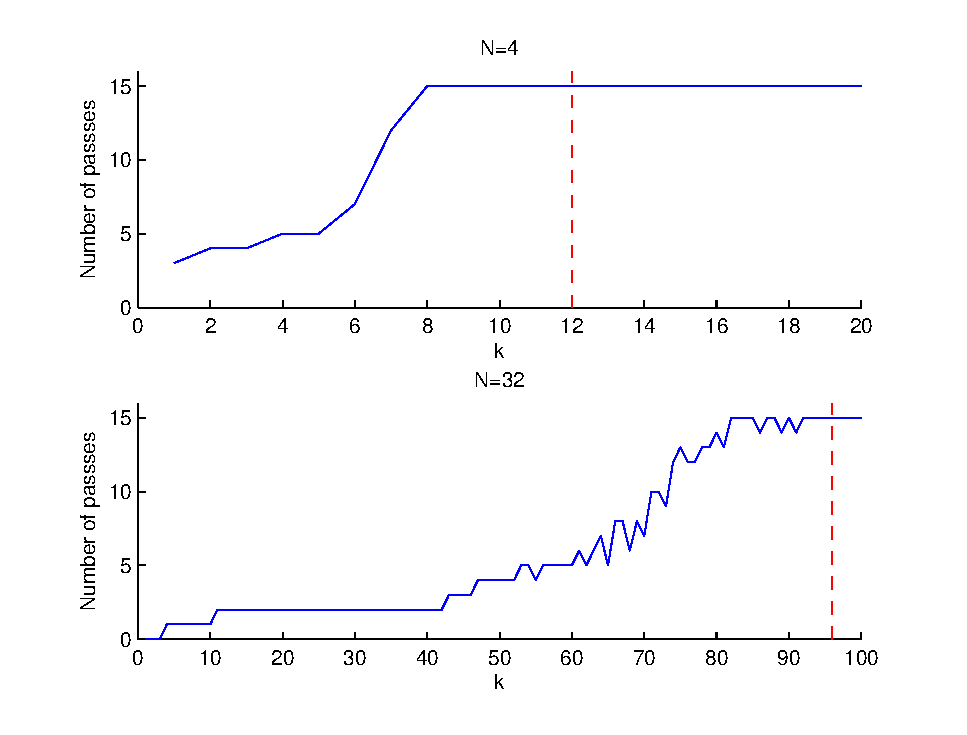
\includegraphics[scale=0.55]{correlation_c_sc.eps} 
\DeclareGraphicsExtensions.
\caption{Small Crush for CI(ISAAC,XORshift)}
\label{Small Crush for CI}
\end{figure}

\subsubsection{Correlation between TestU01 results and $\mathsf{N}$}

To compare the sequences generated with different parameters $\mathsf{N}$ 
in a more quantitative manner, we have set $k=3N+1$, and the same analysis 
for the four CI(X,Y) generators through TestU01 has been repeated. Let us recall 
that the TestU01 suite implements 518 tests and reports $p-$values, which must be 
within $[0.001,0.999]$ for a passing test.

\begin{figure*}
\centering
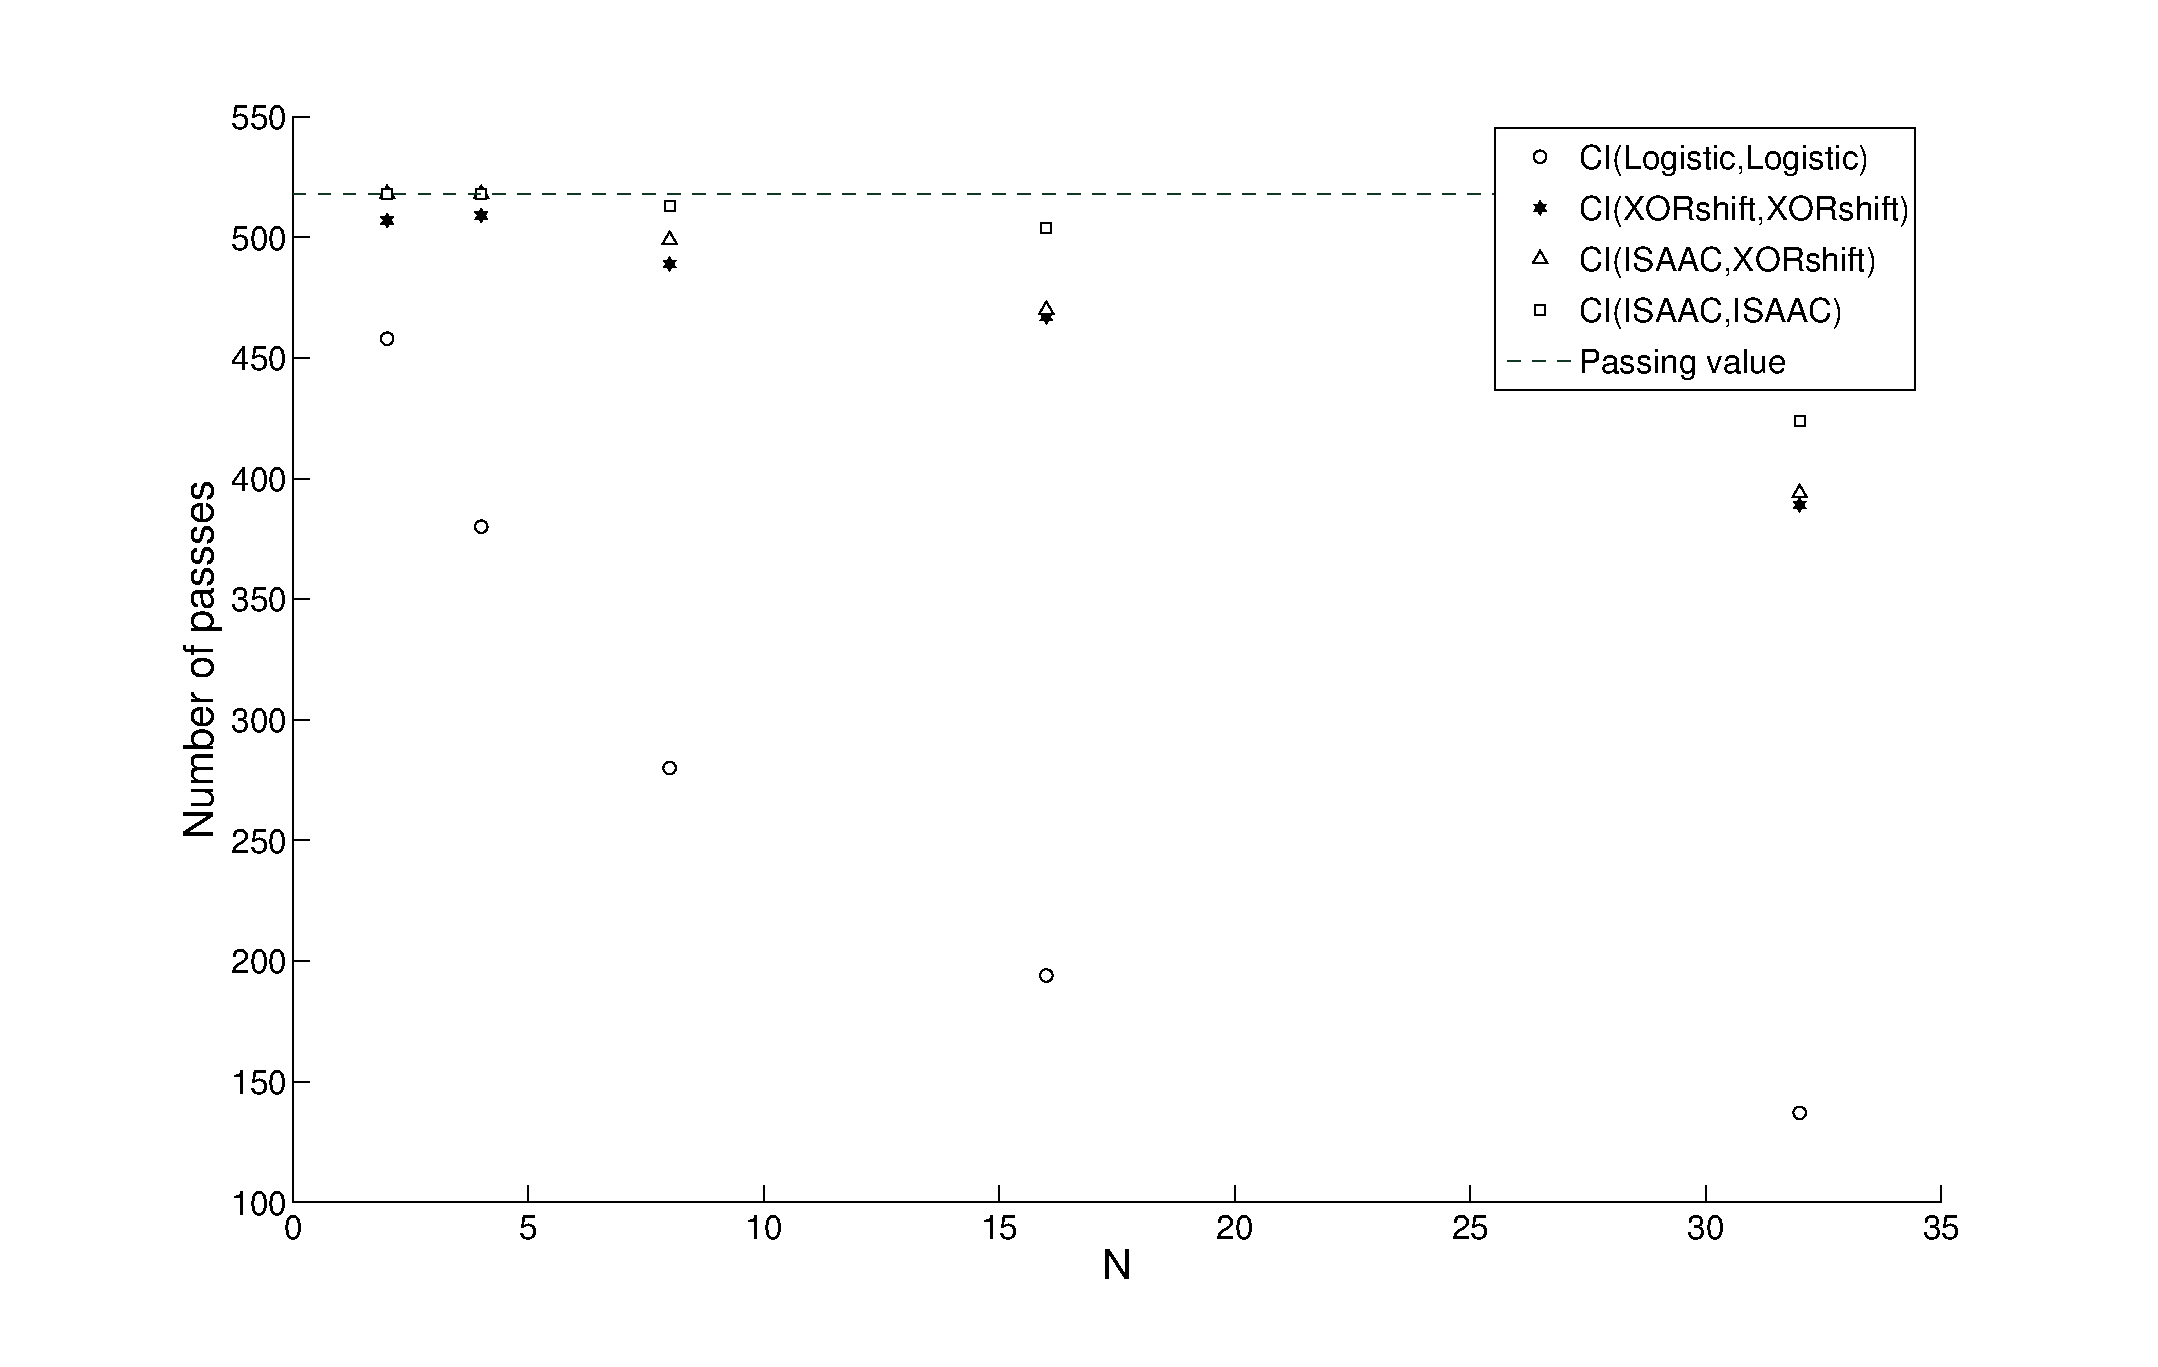
\includegraphics[scale=0.4]{N.eps} 
\DeclareGraphicsExtensions.
\caption{TestU01 results}
\label{TestU01 results}
\end{figure*}

Figure~\ref{TestU01 results} shows the number of passing sequences generated by
the CI(X,Y) PRNGs proposed in this paper, with the same parameters and initial values. % (see the appendix for details).
It can be seen that $\mathsf{N}=4$ gives the best results.

For this reason, it is the default $\mathsf{N}=4$ with $k=12$ mode in following sections.
%As can be seen, the places where a sequence successfully passes most of the tests correspond nicely to the parameters for which $\mathsf{N}=4$.

\subsection{Results of NIST}

In our experiments, 100 sequences (s = 100) of 1,000,000 bits are generated and tested. 
If the value $\mathbb{P}_T$ of any test is smaller than 0.0001, the sequences are considered 
to not be good enough and the generator is unsuitable. Table~\ref{The passing for Version 1 CI} shows 
$\mathbb{P}_T$ of the sequences based on discrete chaotic iterations using different schemes. 
If there are at least two statistical values in a test, this test is marked with an asterisk 
and the average value is computed to characterize the statistical values. 


\begin{table}
\renewcommand{\arraystretch}{1.3}
\caption{NIST SP 800-22 test results ($\mathbb{P}_T$) for Version 1 CI algorithms ($\mathsf{N}=4$)}
\label{The passing for Version 1 CI}
\centering
\begin{tabular}{lcccc}
\toprule
\multirow{4}*{Test name} & \multicolumn{4}{c}{Version 1 CI}\\
&Logistic& XORshift& ISAAC & BBS\\ 
&+& +& + & +\\ 
&Logistic& XORshift& XORshift & XORshift \\ \cmidrule(r){2-5}
Frequency (Monobit) Test 			&0.85138	&0.59554	&0.40119	 & 0.33536 \\ 
Frequency Test within a Block			&0.38382	&0.55442	&0.89776	 & 0.47890 \\ 
Runs Test 					&0.31908	&0.45593	&0.31908	 & 0.89942 \\ 
Longest Run of Ones in a Block Test 		&0.13728	&0.01671	&0.08558	 & 0.02357\\
Binary Matrix Rank Test 			&0.69931	&0.61630	&0.47498	 & 0.25021 \\ 
Discrete Fourier Transform (Spectral) Test	&0.12962	&0.00019	&0.77918	 & 0.08945\\ 
Non-overlapping Template Matching Test* 	&0.48473	&0.53225	&0.53568	 & 0.24587\\ 
Overlapping Template Matching Test 		&0.47498	&0.33453	&0.36691	 & 0.94873 \\ 
Universal Statistical Test 			&0.09657	&0.03292	&0.26224	 & 0.32486\\ 
Linear Complexity Test			&0.41902	&0.40119	&0.61715	 & 0.88345 \\ 
Serial Test* (m=10) 				&0.53427	&0.01339	&0.33453	 & 0.43803 \\ 
Approximate Entropy Test (m=10) 		&0.99146	&0.13728	&0.53414	 & 0.34759 \\ 
Cumulative Sums (Cusum) Test* 			&0.75530	&0.04646	&0.31915	 & 0.23536\\ 
Random Excursions Test* 			&0.65406	&0.50362	&0.50804	 & 0.87633 \\ 
Random Excursions Variant Test* 		&0.55388	&0.34777	&0.48400	& 0.64242\\ \hline
Success 					&15/15		&15/15		&15/15		 & 15/15\\ 
\bottomrule
\end{tabular}
\end{table}


\subsection{Results of Diehard}
\label{Subsec:DieHARD}

Table~\ref{Results of DieHARD battery of tests for Version 1 CI algorithms} gives the results 
derived from applying the DieHARD battery of tests to the PRNGs considered in this work. 

\begin{tiny}
\begin{table}[!t]
\renewcommand{\arraystretch}{1.3}
\caption{Results of DieHARD battery of tests for Version 1 CI algorithms ($\mathsf{N}=4$)}
\label{Results of DieHARD battery of tests for Version 1 CI algorithms}
\centering
\begin{tabular}{llcccc} \toprule
\multirow{4}*{No.} &\multirow{4}*{Test name}& \multicolumn{4}{c}{Version 1 CI}\\
&&Logistic& XORshift& ISAAC&BBS\\ 
&&+& +& + & + \\ 
&&Logistic& XORshift& XORshift&XORshift \\ \cmidrule(r){3-6}

1 & Overlapping Sum &Pass &Pass &Pass&Pass\\
2 & Runs Up 1 &Pass & Pass &Pass&Pass\\
&Runs Down 1 &Pass &Pass &Pass&Pass\\
&Runs Up 2 & Pass &Pass &Pass&Pass\\
&Runs Down 2 &Pass & Pass &Pass&Pass\\
3 & 3D Spheres &Pass &Pass &Pass&Pass\\
4 & Parking Lot &Pass &Pass &Pass&Pass\\
5 & Birthday Spacing &Pass &Pass &Pass&Pass\\
6 & Count the ones 1 &Pass &Pass &Pass&Pass\\
7 &Binary Rank $6 \times 8$ &Pass & Pass &Pass&Pass\\
8 &Binary Rank $31 \times 31$ &Pass &Pass &Pass&Pass\\
9 &Binary Rank $32 \times 32$ &Pass &Pass &Pass&Pass\\
10 &Count the ones 2 &Pass &Pass&Pass&Pass \\
11 &Bit Stream &Pass &Pass&Pass&Pass \\
12 &Craps Wins &Pass &Pass&Pass&Pass \\
&Throws &Pass &Pass &Pass&Pass\\
13 &Minimum Distance &Pass &Pass &Pass&Pass\\
14 &Overlapping Perm. &Pass &Pass &Pass&Pass\\
15 &Squeeze &Pass &Pass&Pass&Pass \\
16 &OPSO &Pass &Pass&Pass&Pass \\
17 &OQSO &Pass &Pass&Pass&Pass \\
18 &DNA &Pass &Pass&Pass &Pass\\
&Number of tests passed &18 &18 &18&18\\\bottomrule
\end{tabular}
\end{table}
\end{tiny}

\subsection{Results of comparative test parameters}

\begin{table}[!t]
\renewcommand{\arraystretch}{1.3}
\caption{Comparative test parameters for Version 1 CI(X,Y) with a $10^7$ bits sequence ($\mathsf{N}=4$)}
\label{Comparison2 for Version 1 CI algorithms}
\centering
\begin{tabular}{lccccc}
\toprule
\multirow{4}*{Method} &\multirow{4}*{Threshold values} 	& \multicolumn{4}{c}{Version 1 CI}\\
&&Logistic& XORshift& ISAAC&BBS \\ 
&&+& +& + & + \\ 
&&Logistic& XORshift& XORshift&XORshift \\ \cmidrule(r){3-6}
Monobit			&3.8415		&1.0368		&3.5689		&0.0569		&0.6641 \\ \hline
Serial		&5.9915		&1.1758		&3.5765		&0.9828		&0.6506\\ \hline
Poker			&316.9194	&269.0607	&222.3683	&243.8415	&262.6440\\ \hline
Runs 			&55.0027	&36.5479	&28.4237	&29.3195	&30.3116 \\ \hline
Autocorrelation		&1.6449		&0.4054		&0.3403		&0.6141		&0.9455\\ \bottomrule
\end{tabular}
\end{table}


We show in Table~\ref{Comparison2 for Version 1 CI algorithms} a comparison between Version 1
CI(Logistic, Logistic), Version 1 CI(XORshift, XORshift), Version 1 CI(ISAAC, XORshift), 
and Version 1 CI(BBS, XORshift). %The comparative test is related to the duration needed by each algorithm to generate a $10^7$ bits long sequence. 


\subsection{Results of TestU01}
In a sound theoretical basis, a PRNG based on discrete chaotic iterations (CI) 
is a composite generator which combines the features of two PRNGs. The first generator constitutes 
the initial condition of the chaotic dynamical system. The second generator randomly chooses which outputs 
of the chaotic system must be returned. The intention of this combination is to cumulate the effects of chaotic 
and random behaviors, to improve the statistical and security properties relative to each generator taken alone.

This PRNG based on discrete chaotic iterations may utilize any reasonable RNG as inputs. 
For demonstration purposes, Logistic map, XORshift and ISAAC are adopted here. 

Table~\ref{TestU01 for Version 1 CI} gives the results derived from applying the TestU01 battery 
of tests to the PRNGs considered in this work.
\begin{table}[!t]
\renewcommand{\arraystretch}{1.3}
\caption{TestU01 Statistical Test for Version 1 CI algorithms ($\mathsf{N}=4$)}
\label{TestU01 for Version 1 CI}
\centering
\begin{tabular}{lcccccc}
\toprule
\multirow{4}*{Test name} &&& \multicolumn{4}{c}{Version 1 CI}\\
&&&Logistic& XORshift& ISAAC&BBS\\ 
&&&+& +& + & + \\ 
&&&Logistic& XORshift& XORshift&XORshift\\ \cmidrule(r){4-7}
Rabbit 				&$32\times10^9$ bits	&38	&7 	&2 	&0 	&2	 \\
Alphabit 			&$32\times10^9$ bits	&17 	& 3	&0 	&0 	&2	 \\
Pseudo DieHARD 			&Standard		&126 	&0 	&0 	&0 	&0	\\
FIPS\_140\_2 			&Standard		&16 	&0 	&0	&0 	&0	\\
Small Crush 			&Standard		&15 	&2 	&0	&0 	&0	 \\
Crush 				&Standard		&144 	&47 	&4 	&0 	&10	 \\
Big Crush 			&Standard		&160 	&79 	&3 	&0	&41	 \\ \hline
Number of failures 		& 			&518 	&138 	&9 	&0 	&55	 \\
\bottomrule
\end{tabular}
\end{table}


\subsection{Conclusion}


Our Version 1 CI PRNG based on discrete chaotic iterations combines the features of two PRNGs, in order to improve 
their statistical properties. BBS, Logistic map, XORshift, and ISAAC are adopted here for demonstration purposes. 
The results of comparative test parameters confirm that the proposed CI PRNGs are all able to pass these tests.
Statistical results of comparative test parameters for both CI(XORshift, XORshift) and CI(ISAAC, XORshift) 
(proven to be cryptographically secure )are better
for most of the parameters, leading to the conclusion that these generators are more secure than the others. 
This improvement clearly appears in the TestU01 results: i.e. XORshift alone fails 142 of these tests, 
whereasCI(XORshift, XORshift) only fails 9 out of 518.
In other words, in addition of having chaotic properties, our PRNG based on discrete chaotic iterations 
can pass more performed tests than its individual components taken alone. 


\section{Test results and comparative analysis for Version 2 CI}
\label{Test for Version 2 CI}
\subsection{Results of NIST}
\label{Results of NISTfor Version 2 CI}
In our experiments, 100 sequences (s = 100) of 
1,000,000 bits are generated and tested. If the value 
$\mathbb{P}_T$ of any test is smaller than 0.0001, the sequences are 
considered to not be good enough and the generator is unsuitable. 
Table~\ref{The passing rate1} and Table~\ref{The passing for Version 2 CI} n
show $\mathbb{P}_T$ of the sequences based on discrete chaotic iterations using different schemes.
If there are at least two statistical values in a test, this test is marked with an asterisk and 
the average value is computed to characterize the statistical values. 

\begin{table}[!t]
\renewcommand{\arraystretch}{1.3}
\caption{SP 800-22 test results ($\mathbb{P}_T$) for Version 2 CI(XORshift, XORshift)$\mathsf{N}=32$}
\label{The passing rate1}
\centering
\begin{tabular}{lcccc}
\toprule
\multirow{2}*{Method} & \multicolumn{3}{c}{Version 2 CI}\\
 & $m^n=y^n~mod~N$&no mark&$g_2()$\\ \cmidrule(r){2-4}
%$w^{j}$ & $\{1,..,8\}$ & $\{1,..,8\}$ & $\{1,..,8\}$ & $\{1,..,5\}$ & $\{1,..,5\}$ &$\{1,..,5\}$ \\ \hline \hline
Frequency (Monobit) Test 			&0.00040	&0.08556		&0.41943\\ 
Frequency Test within a Block			&0		&0			&0.67862\\ 
Runs Test					&0.28966	&0.55448		&0.33452\\ 
Longest Run of Ones in a Block Test 		&0.01096	&0.43723		&0.88313 \\ 
Binary Matrix Rank Test			&0		&0.65794		&0.75972\\ 
Discrete Fourier Transform (Spectral) Test 	&0		&0			&0.00085 \\ 
Non-overlapping Template Matching Test* 	&0.02007	&0.37333		&0.51879\\ 
Overlapping Template Matching Test		&0		&0	 	 	&0.24924\\ 
Maurer's ``Universal Statistical'' Test	&0.69936	&0.96424		&0.12963\\ 
Linear Complexity Test 				&0.36699	&0.92423	 	&0.35045\\ 
Serial Test* (m=10) 				&0		&0.28185	 	&0.25496\\ 
Approximate Entropy Test (m=10) 		&0		&0.38381	 	&0.75971\\ 
Cumulative Sums (Cusum) Test* 			&0		&0			&0.34245\\ 
Random Excursions Test* 			&0.46769	&0.34788	 	&0.18977\\ 
Random Excursions Variant Test* 		&0.28779	&0.46505		&0.26563\\ \hline
Success 					&8/15		&11/15			&15/15\\ 
\bottomrule
\end{tabular}
\end{table}

We can conclude from Table \ref{The passing rate1} that the worst 
situations are obtained with the Version 2 CI ($m^n=y^n~mod~N$) and 
Version 2 CI (no mark) generators. %: they just can be observed that 8 and 11 out of 15 of the tests are failed. However,
Version 2 CI ($m^n=g_2(y^n)$) as Version 2 CI ($m^n=g_1(y^n)$) in 
Table~\ref{The passing for Version 2 CI} has almost all successfully passed the 
NIST statistical test suite, the structure of mixing BBS and XORshift can not pass 
the tests of ``Approximate Entropy'' and ``Serial'', the reason might relates to 
poor statistical properties of BBS in long term output, though it can be treated as 
cryptographically secure.

\begin{table}[!t]
\renewcommand{\arraystretch}{1.3}
\caption{NIST SP 800-22 test results ($\mathbb{P}_T$) for Version 2 CI algorithms}
\label{The passing for Version 2 CI}
\centering
\begin{tabular}{lccc}
\toprule
\multirow{4}*{Test name} & \multicolumn{3}{c}{Version 2 CI}\\
& XORshift& ISAAC &BBS\\ 
& +& + & + \\ 
& XORshift& XORshift&XORshift\\\cmidrule(r){2-4}
Frequency (Monobit) Test 			&0.47498 		&0.88317		&0.83430 \\ 
Frequency Test within a Block			&0.89776		&0.40119		&0.33453\\ 
Runs Test 					&0.81653		&0.31908		&0.00576\\ 
Longest Run of Ones in a Block Test 		&0.79813		&0.06688		&0.47498 \\
Binary Matrix Rank Test 			&0.26224		&0.88317		&0.69931\\ 
Discrete Fourier Transform (Spectral) Test	&0.00716		&0.33453		&0.59559 \\ 
Non-overlapping Template Matching Test* 	&0.44991		&0.46467		&0.51446 \\ 
Overlapping Template Matching Test 		&0.51412		&0.69931		&0.88317\\ 
Universal Statistical Test 			&0.67868		&0.24928		&0.06282 \\ 
Linear Complexity Test			&0.65793		&0.65793		&0.94630 \\ 
Serial Test* (m=10) 				&0.42534		&0.90619		&0.00000 \\ 
Approximate Entropy Test (m=10) 		&0.63719		&0.22482		&0.00000\\ 
Cumulative Sums (Cusum) Test* 			&0.27968		&0.84065		&0.14139 \\ 
Random Excursions Test* 			&0.28740		&0.30075		&0.34625 \\ 
Random Excursions Variant Test* 		&0.48668		&0.34294		&0.55048\\ \hline
Success 					& 15/15			&15/15		&13/15	 \\ 
\bottomrule
\end{tabular}
\end{table}

\subsection{Results of Diehard}
Table~\ref{Results of DieHARD battery of tests for Version 2 CI algorithms} gives 
the results derived from applying the DieHARD battery of tests to the PRNGs considered in this work. 
Very the same reason as NIST test suite's results, mixing of BBS and XORshift is not able to pass them all.

\begin{tiny}
\begin{table}[!t]
\renewcommand{\arraystretch}{1.3}
\caption{Results of DieHARD battery of tests for Version 2 CI algorithms ($\mathsf{N}=32$)}
\label{Results of DieHARD battery of tests for Version 2 CI algorithms}
\centering
\begin{tabular}{llcccc} \toprule
\multirow{3}*{No.} &\multirow{3}*{Test name} & \multicolumn{4}{c}{Version 2 CI}\\
&&Logistic& XORshift& ISAAC&BBS \\ 
&&+& +& + & + \\ 
&&Logistic& XORshift& XORshift&XORshift \\ \cmidrule(r){3-6}
1 & Overlapping Sum &Pass &Pass &Pass&Pass\\
2 & Runs Up 1 &Pass & Pass &Pass&Pass\\
&Runs Down 1 &Pass &Pass &Pass&Pass\\
&Runs Up 2 & Pass &Pass &Pass&Pass\\
&Runs Down 2 &Pass & Pass &Pass&Pass\\
3 & 3D Spheres &Pass &Pass &Pass&Pass\\
4 & Parking Lot &Pass &Pass &Pass&Pass\\
5 & Birthday Spacing &Pass &Pass &Pass&Pass\\
6 & Count the ones 1 &Pass &Pass &Pass&Fail\\
7 &Binary Rank $6 \times 8$ &Pass & Pass &Pass&Pass\\
8 &Binary Rank $31 \times 31$ &Pass &Pass &Pass&Pass\\
9 &Binary Rank $32 \times 32$ &Pass &Pass &Pass&Pass\\
10 &Count the ones 2 &Pass &Pass&Pass&Pass \\
11 &Bit Stream &Pass &Pass&Pass&Pass \\
12 &Craps Wins &Pass &Pass&Pass&Pass \\
&Throws &Pass &Pass &Pass&Pass\\
13 &Minimum Distance &Pass &Pass &Pass&Pass\\
14 &Overlapping Perm. &Pass &Pass &Pass&Pass\\
15 &Squeeze &Pass &Pass&Pass&Pass \\
16 &OPSO &Pass &Pass&Pass&Pass \\
17 &OQSO &Pass &Pass&Pass&Pass \\
18 &DNA &Pass &Pass&Pass &Fail\\
&Number of tests passed &18 &18 &18&16\\\bottomrule
\end{tabular}
\end{table}
\end{tiny}

\subsection{Results of comparative test parameters}



\begin{table}[!t]
\renewcommand{\arraystretch}{1.3}
\caption{Comparative test parameters for Version 2 CI(X,Y) with a $10^7$ bits sequence ($\mathsf{N}=32$)}
\label{Comparison2 for Version 2 CI algorithms}
\centering
\begin{tabular}{lcccc}
\toprule
\multirow{4}*{Method} &\multirow{4}*{Threshold values} 	& \multicolumn{3}{c}{Version 2 CI}\\
&& XORshift& ISAAC&BBS\\ 
&& +& + & + \\ 
&& XORshift& XORshift&XORshift \\ \cmidrule(r){2-5}
Monobit			&3.8415				&3.5689		&0.9036		&0.5788 \\ \hline
Serial		&5.9915				&3.5765		&1.1229		&0.7378\\ \hline
Poker			&316.9194			&123.6831	&173.8604		&319.8609\\ \hline
Runs 			&55.0027			&28.4237	&40.4606	&49.4057 \\ \hline
Autocorrelation		&1.6449				&0.3403		&0.1245		&-2.0276 \\ \bottomrule
\end{tabular}
\end{table}

We show in Table~\ref{Comparison2 for Version 2 CI algorithms} 
a comparison between Version 2 CI(XORshift, XORshift), 
Version 2 CI(ISAAC, XORshift), and Version 2 CI(BBS, XORshift). %The comparative test is related to the duration needed by each algorithm to generate a $10^7$ bits long sequence. 

\subsection{Results of TestU01}


Table~\ref{TestU01 for Version 2 CI} gives 
the results derived from applying the TestU01 battery of tests to the PRNGs considered in this work.
\begin{table}[!t]
\renewcommand{\arraystretch}{1.3}
\caption{TestU01 Statistical Test for Version 2 CI algorithms ($\mathsf{N}=32$)}
\label{TestU01 for Version 2 CI}
\centering
\begin{tabular}{lccccc}
\toprule
\multirow{4}*{Test name} &&& \multicolumn{3}{c}{Version 2 CI}\\
&&&Logistic& ISAAC&BBS\\ 
&&&+& +& + \\ 
&&&Logistic& XORshift&XORshift\\ \cmidrule(r){4-6}
Rabbit 				&$32\times10^9$ bits	&38	&0 	&0 	& 7		 \\
Alphabit 			&$32\times10^9$ bits	&17 	&0 	&0 	& 6		 \\
Pseudo DieHARD 			&Standard		&126 	&0 	&0 	& 1		\\
FIPS\_140\_2 			&Standard		&16 	&0 	&0 	& 0		\\
Small Crush 			&Standard		&15 	&0	&0	& 3		 \\
Crush 				&Standard		&144 	&0 	&0 	& 11		 \\
Big Crush 			&Standard		&160 	&0 	&0 	& 29		 \\ \hline
Number of failures 		& 			& 	&0 	&0	& 57		 \\
\bottomrule
\end{tabular}
\end{table}


\subsection{Conclusion}
In a sound theoretical basis, a New PRNG 
based on discrete chaotic iterations (CI) is a composite generator which 
combines the features of two PRNGs. The first generator constitutes the initial 
condition of the chaotic dynamical system. The second generator randomly chooses which 
outputs of the chaotic system must be returned. The intention of this combination is to cumulate 
the effects of chaotic and random behaviors, to improve the statistical and security properties 
relative to each generator taken alone.

This Version 2 CI PRNG based on discrete chaotic iterations may utilize any 
reasonable RNG as inputs. For demonstration purposes, XORshift and ISAAC are adopted here. 

The results of the TestU01, NIST, Comparative test parameters and DieHARD batteries of tests 
confirm that the proposed Version 2 CI PRNGs are all able to pass these tests. 
And it is better than Version 1 CI algorithms

The improvement clearly appears in the TestU01 results: i.e. XORshift alone fails 142 
of these tests, whereasVersion 1 CI(XORshift, XORshift) fails 9 out of 518, 
Version 2 CI(XORshift, XORshift) can pass all the tests. However for CI(BBS, XORshift), 
to choose $m$ fluents more than to choose $k$ in the output quality, Version 2 CI shows
worse performance than Version 1.

Detail comparative analysis will be presented in the latter section.


\section{Test results and comparative analysis for Version 3 LUT CI}
\subsection{Results of NIST}
\label{Results of NISTfor Version 3 CI}
In our experiments, 100 sequences (s = 100) of 
1,000,000 bits are generated and tested. If the value 
$\mathbb{P}_T$ of any test is smaller than 0.0001, the sequences are 
considered to not be good enough and the generator is unsuitable. 
If there are at least two statistical values in a test, this test is marked with an asterisk and 
the average value is computed to characterize the statistical values. 

The Version 3 LUT CI we used in test are all in 
$N = 4$ bits format. We can conclude from Table~\ref{The passing for Version 3 LUT CI} that except mixture of BBS and XORshift, all others have successfully passed the NIST statistical test suite. The same reason as previously described,
BBS's poor statistical performance leads outputs of LUT-1 distribute not very uniform. 

\begin{table}
\renewcommand{\arraystretch}{1.3}
\caption{NIST SP 800-22 test results ($\mathbb{P}_T$) for Version 3 LUT CI algorithms}
\label{The passing for Version 3 LUT CI}
\centering
\begin{tabular}{lccc}
\toprule
\multirow{4}*{Test name} & \multicolumn{3}{c}{Version 3 LUT CI}\\
& XORshift& ISAAC &BBS\\ 
& +& + & + \\ 
& XORshift& XORshift&XORshift\\\cmidrule(r){2-4}
Frequency (Monobit) Test 			&0.32435 		&0.33171		&0.00000 \\ 
Frequency Test within a Block			&0.85643		&0.42327		&0.13233\\ 
Runs Test 					&0.11623		&0.31908		&0.00000\\ 
Longest Run of Ones in a Block Test 		&0.74254		&0.86688		&0.00000 \\
Binary Matrix Rank Test 			&0.23224		&0.88317		&0.90311\\ 
Discrete Fourier Transform (Spectral) Test	&0.12316		&0.34578		&0.59559 \\ 
Non-overlapping Template Matching Test* 	&0.43295		&0.32637		&0.00000 \\ 
Overlapping Template Matching Test 		&0.31472		&0.55915		&0.00000\\ 
Universal Statistical Test 			&0.37864		&0.24925		&0.06282 \\ 
Linear Complexity Test			&0.65723		&0.31793		&0.94630 \\ 
Serial Test* (m=10) 				&0.43532		&0.55190		&0.00000 \\ 
Approximate Entropy Test (m=10) 		&0.34254		&0.12482		&0.00000\\ 
Cumulative Sums (Cusum) Test* 			&0.11272		&0.04065		&0.14139 \\ 
Random Excursions Test* 			&0.02003		&0.32275		&0.34625 \\ 
Random Excursions Variant Test* 		&0.43554		&0.234294		&0.55048\\ \hline
Success 					& 15/15			&15/15		&8/15	 \\ 
\bottomrule
\end{tabular}
\end{table}

\subsection{Results of Diehard}
Table~\ref{Results of DieHARD battery of tests for Version 3 LUT CI algorithms} gives 
the results derived from applying the DieHARD battery of tests to the PRNGs considered in this work. 
Very the same reason as NIST test suite's results, mixture of BBS and XORshift is not able to pass them all, though it is proven to be cryptographically secure, however its poor performance in statistical deny its qualify to be a good generator.

\begin{tiny}
\begin{table}
\renewcommand{\arraystretch}{1.3}
\caption{Results of DieHARD battery of tests for Version 3 LUT CI algorithms ($\mathsf{N}=4$)}
\label{Results of DieHARD battery of tests for Version 3 LUT CI algorithms}
\centering
\begin{tabular}{llcccc} \toprule
\multirow{3}*{No.} &\multirow{3}*{Test name} & \multicolumn{4}{c}{Version 3 CI}\\
&&Logistic& XORshift& ISAAC&BBS \\ 
&&+& +& + & + \\ 
&&Logistic& XORshift& XORshift&XORshift \\ \cmidrule(r){3-6}
1 & Overlapping Sum &Pass &Pass &Pass&Fail\\
2 & Runs Up 1 &Pass & Pass &Pass&Pass\\
&Runs Down 1 &Pass &Pass &Pass&Pass\\
&Runs Up 2 & Pass &Pass &Pass&Pass\\
&Runs Down 2 &Pass & Pass &Pass&Pass\\
3 & 3D Spheres &Pass &Pass &Pass&Fail\\
4 & Parking Lot &Pass &Pass &Pass&Pass\\
5 & Birthday Spacing &Pass &Pass &Pass&Fail\\
6 & Count the ones 1 &Pass &Pass &Pass&Fail\\
7 &Binary Rank $6 \times 8$ &Pass & Pass &Pass&Pass\\
8 &Binary Rank $31 \times 31$ &Pass &Pass &Pass&Fail\\
9 &Binary Rank $32 \times 32$ &Pass &Pass &Pass&Fail\\
10 &Count the ones 2 &Pass &Pass&Pass&Fail \\
11 &Bit Stream &Pass &Pass&Pass&Pass \\
12 &Craps Wins &Pass &Pass&Pass&Fail \\
&Throws &Pass &Pass &Pass&Pass\\
13 &Minimum Distance &Pass &Pass &Pass&Pass\\
14 &Overlapping Perm. &Pass &Pass &Pass&Pass\\
15 &Squeeze &Pass &Pass&Pass&Pass \\
16 &OPSO &Pass &Pass&Pass&Fail \\
17 &OQSO &Pass &Pass&Pass&Fail \\
18 &DNA &Pass &Pass&Pass &Fail\\
&Number of tests passed &18 &18 &18&8\\\bottomrule
\end{tabular}
\end{table}
\end{tiny}

\subsection{Results of comparative test parameters}



\begin{table}
\renewcommand{\arraystretch}{1.3}
\caption{Comparative test parameters for Version 3 CI(X,Y) with a $10^7$ bits sequence ($\mathsf{N}=4$)}
\label{Comparison2 for Version 3 CI algorithms}
\centering
\begin{tabular}{lcccc}
\toprule
\multirow{4}*{Method} &\multirow{4}*{Threshold values} 	& \multicolumn{3}{c}{Version 3 CI}\\
&& XORshift& ISAAC&BBS\\ 
&& +& + & + \\ 
&& XORshift& XORshift&XORshift \\ \cmidrule(r){2-5}
Monobit			&3.8415				&3.5689		&0.9036		&1.5788 \\ \hline
Serial		&5.9915				&3.5765		&1.1229		&3.378\\ \hline
Poker			&316.9194			&123.6831	&173.8604		&409.3320\\ \hline
Runs 			&55.0027			&28.4237	&40.4606	&88.4153 \\ \hline
Autocorrelation		&1.6449				&0.3403		&0.1245		&-2.0276 \\ \bottomrule
\end{tabular}
\end{table}

We show in Table~\ref{Comparison2 for Version 3 CI algorithms} 
a comparison between Version 3 CI(XORshift, XORshift), 
Version 3 CI(ISAAC, XORshift), and Version 3 CI(BBS, XORshift). 
According to these $10^7$ bits long sequence tests, again (BBS, XORshift) shows 
the worst performance. 

\subsection{Results of TestU01}


Table~\ref{TestU01 for Version 3 CI} gives 
the results derived from applying the TestU01 battery of tests to the PRNGs considered in this work.
\begin{table}
\renewcommand{\arraystretch}{1.3}
\caption{TestU01 Statistical Test for Version 3 CI algorithms ($\mathsf{N}=4$)}
\label{TestU01 for Version 3 CI}
\centering
\begin{tabular}{lccccc}
\toprule
\multirow{4}*{Test name} &&& \multicolumn{3}{c}{Version 3 CI}\\
&&&Logistic& ISAAC&BBS\\ 
&&&+& +& + \\ 
&&&Logistic& XORshift&XORshift\\ \cmidrule(r){4-6}
Rabbit 				&$32\times10^9$ bits	&38	&0 	&0 	& 18		 \\
Alphabit 			&$32\times10^9$ bits	&17 	&0 	&0 	& 	8	 \\
Pseudo DieHARD 			&Standard		&126 	&0 	&0 	& 11	\\
FIPS\_140\_2 			&Standard		&16 	&0 	&0 	& 0		\\
Small Crush 			&Standard		&15 	&0	&0	& 7		 \\
Crush 				&Standard		&144 	&0 	&0 	& 51		 \\
Big Crush 			&Standard		&160 	&0 	&0 	& 77		 \\ \hline
Number of failures 		& 			& 	&0 	&0	& 165		 \\
\bottomrule
\end{tabular}
\end{table}


\subsection{Conclusion}

By using some well-defined Lookupand due to the rewrite of the way to generate strategies, the generator based on chaotic iterations works faster and is more secure. The speed of LUT CI can be hugely improved compare to Version 1 and Version 2 CI. As the tests shown, it also can offer a sufficient speed and level of security.

This Version 3 CI PRNG based on discrete chaotic iterations may utilize any 
reasonable RNG as inputs. For demonstration purposes, XORshift, BBS, ISAAC are adopted here. 

The results of the TestU01, NIST, Comparative test parameters and DieHARD batteries of tests 
confirm that the proposed Version 3 CI PRNGs are all able to pass these tests. 
And it is better than Version 1 CI algorithms, also use less computation source than Version 2 CI algorithm. 



\section{Tests results and comparative analysis for Version 4 CI}
\label{test for Version 4 CI}
\subsection{Results of NIST}
\label{Results of NIST for Version 4 CI}
In our experiments, 100 sequences (s = 100) of 
1,000,000 bits are generated and tested. If the value 
$\mathbb{P}_T$ of any test is smaller than 0.0001, the sequences are 
considered to not be good enough and the generator is unsuitable. 
If there are at least two statistical values in a test, this test is marked with an asterisk and 
the average value is computed to characterize the statistical values. 

The Version 4 CI we used in test are all in 
$N = 32$ bits format. We can conclude from Table~\ref{The passing for Version 4 CI} that all PRNGs have successfully passed the NIST statistical test suite. Even with BBS's not good property, the Version 4 CIPRNG (BBS, Xorshift) still can perform well.

\begin{table}
\renewcommand{\arraystretch}{1.3}
\caption{NIST SP 800-22 test results ($\mathbb{P}_T$) for Version 3 LUT CI algorithms}
\label{The passing for Version 4 CI}
\centering
\begin{tabular}{lccc}
\toprule
\multirow{4}*{Test name} & \multicolumn{3}{c}{Version 4 CI}\\
& XORshift& ISAAC &BBS\\ 
& +& + & + \\ 
& XORshift& XORshift&XORshift\\\cmidrule(r){2-4}
Frequency (Monobit) Test 			&0.21414 		&0.43622		&0.24563 \\ 
Frequency Test within a Block			&0.23423		&0.43536		&0.13233\\ 
Runs Test 					&0.56471		&0.23425		&0.23562 \\ 
Longest Run of Ones in a Block Test 		&0.33252		&0.86688		&0.12346 \\
Binary Matrix Rank Test 			&0.01450		&0.25689		&0.90311\\ 
Discrete Fourier Transform (Spectral) Test	&0.25462		&0.32324		&0.59559 \\ 
Non-overlapping Template Matching Test* 	&0.79521		&0.32637		&0.03984 \\ 
Overlapping Template Matching Test 		&0.69342		&0.55915		&0.13839\\ 
Universal Statistical Test 			&0.44654		&0.24925		&0.06282 \\ 
Linear Complexity Test			&0.97319		&0.31793		&0.54630 \\ 
Serial Test* (m=10) 				&0.58993		&0.55190		&0.98234 \\ 
Approximate Entropy Test (m=10) 		&0.39284		&0.12482		&0.12345\\ 
Cumulative Sums (Cusum) Test* 			&0.43582		&0.04065		&0.14139 \\ 
Random Excursions Test* 			&0.92001		&0.32275		&0.34625 \\ 
Random Excursions Variant Test* 		&0.24567		&0.234294		&0.55048\\ \hline
Success 					& 15/15			&15/15		&15/15	 \\ 
\bottomrule
\end{tabular}
\end{table}

\subsection{Results of Diehard}
Table~\ref{Results of DieHARD battery of tests for Version 4 CI algorithms} gives 
the results derived from applying the DieHARD battery of tests to the PRNGs considered in this work. The same as NIST test suite's results, the mixing of BBS and XORshift shows better performance than in the other CI Versions, all generators are successfully pass the tests.

\begin{tiny}
\begin{table}
\renewcommand{\arraystretch}{1.3}
\caption{Results of DieHARD battery of tests for Version 4 CI algorithms ($\mathsf{N}=4$)}
\label{Results of DieHARD battery of tests for Version 4 CI algorithms}
\centering
\begin{tabular}{llcccc} \toprule
\multirow{3}*{No.} &\multirow{3}*{Test name} & \multicolumn{4}{c}{Version 4 CI}\\
&&Logistic& XORshift& ISAAC&BBS \\ 
&&+& +& + & + \\ 
&&XORshift& XORshift& XORshift&XORshift \\ \cmidrule(r){3-6}
1 & Overlapping Sum &Pass &Pass &Pass&Pass\\
2 & Runs Up 1 &Pass & Pass &Pass&Pass\\
&Runs Down 1 &Pass &Pass &Pass&Pass\\
&Runs Up 2 & Pass &Pass &Pass&Pass\\
&Runs Down 2 &Pass & Pass &Pass&Pass\\
3 & 3D Spheres &Pass &Pass &Pass&Pass\\
4 & Parking Lot &Pass &Pass &Pass&Pass\\
5 & Birthday Spacing &Pass &Pass &Pass&Pass\\
6 & Count the ones 1 &Pass &Pass &Pass&Pass\\
7 &Binary Rank $6 \times 8$ &Pass & Pass &Pass&Pass\\
8 &Binary Rank $31 \times 31$ &Pass &Pass &Pass&Pass\\
9 &Binary Rank $32 \times 32$ &Pass &Pass &Pass&Pass\\
10 &Count the ones 2 &Pass &Pass&Pass&Pass \\
11 &Bit Stream &Pass &Pass&Pass&Pass \\
12 &Craps Wins &Pass &Pass&Pass&Pass \\
&Throws &Pass &Pass &Pass&Pass\\
13 &Minimum Distance &Pass &Pass &Pass&Pass\\
14 &Overlapping Perm. &Pass &Pass &Pass&Pass\\
15 &Squeeze &Pass &Pass&Pass&Pass \\
16 &OPSO &Pass &Pass&Pass&Pass \\
17 &OQSO &Pass &Pass&Pass&Pass \\
18 &DNA &Pass &Pass&Pass &Pass\\
&Number of tests passed &18 &18 &18&18\\\bottomrule
\end{tabular}
\end{table}
\end{tiny}

\subsection{Results of comparative test parameters}



\begin{table}
\renewcommand{\arraystretch}{1.3}
\caption{Comparative test parameters for Version 4 CI(X,Y) with a $10^7$ bits sequence ($\mathsf{N}=32$)}
\label{Comparison2 for Version 4 CI algorithms}
\centering
\begin{tabular}{lcccc}
\toprule
\multirow{4}*{Method} &\multirow{4}*{Threshold values} 	& \multicolumn{3}{c}{Version 3 CI}\\
&& XORshift& ISAAC&BBS\\ 
&& +& + & + \\ 
&& XORshift& XORshift&XORshift \\ \cmidrule(r){2-5}
Monobit			&0.8115				&1.0689		&0.9036		&0.5788 \\ \hline
Serial		&2.3312				&0.5765		&1.0229		&1.378\\ \hline
Poker			&112.2190			&123.6831	&133.8604		&79.3320\\ \hline
Runs 			&33.0027			&28.4237	&13.4606	&12.4153 \\ \hline
Autocorrelation		&0.6449				&1.3403		&0.1845		&-0.7276 \\ \bottomrule
\end{tabular}
\end{table}

We show in Table~\ref{Comparison2 for Version 4 CI algorithms} 
a comparison between Version 4 CI(XORshift, XORshift), 
Version 4 CI(ISAAC, XORshift), and Version 4 CI(BBS, XORshift). 
According to these $10^7$ bits long sequence tests, they all show very good statistical performance.

\subsection{Results of TestU01}
Table~\ref{TestU01 for Version 4 CI} gives 
the results derived from applying the TestU01 battery of tests to the PRNGs considered in this work.
\begin{table}
\renewcommand{\arraystretch}{1.3}
\caption{TestU01 Statistical Test for Version 4 CI algorithms ($\mathsf{N}=4$)}
\label{TestU01 for Version 4 CI}
\centering
\begin{tabular}{lccccc}
\toprule
\multirow{4}*{Test name} &&& \multicolumn{3}{c}{Version 4 CI}\\
&&&Logistic& ISAAC&BBS\\ 
&&&+& +& + \\ 
&&&XORshift& XORshift&XORshift\\ \cmidrule(r){4-6}
Rabbit 				&$32\times10^9$ bits	&0	&0 	&0 	& 0		 \\
Alphabit 			&$32\times10^9$ bits	&0 	&0 	&0 	& 	0	 \\
Pseudo DieHARD 			&Standard		&0 	&0 	&0 	& 0	\\
FIPS\_140\_2 			&Standard		&0 	&0 	&0 	& 0		\\
Small Crush 			&Standard		&0 	&0	&0	& 0		 \\
Crush 				&Standard		&0 	&0 	&0 	& 0		 \\
Big Crush 			&Standard		&0 	&0 	&0 	& 0		 \\ \hline
Number of failures 		& 			&0 	&0 	&0	& 0		 \\
\bottomrule
\end{tabular}
\end{table}


\subsection{Conclusion}

The new Version CI cause a great compromise among cryptographically secure property, statistical performance and efficiency, it is very suitable used in hardware implementation, also the software implementation.

This Version 4 CI PRNG based on discrete chaotic iterations is able to utilize any reasonable RNG as inputs. For demonstration purposes, XORshift, BBS, ISAAC are adopted here. 

The results of the TestU01, NIST, Comparative test parameters and DieHARD batteries of tests confirm that the proposed Version 4 CI PRNGs are all able to pass these tests. And it is better than the other CI algorithms, it is very adaptive to parallel application. 

\section{Assessment of two chaotic iterations schemes based on XORshift Generator}
In this section, the comparison between Version 1-4 CIPRNG in statistical aspect. For fairy, all the tested CIPRNGs are using XORshift as is subset PRNGs, and the assignments of the parameters are the most optimized according to the experiments: thus the $N$ for Version 1 and 3 CI is $4$, for Version 2 and 4 is $32$.

\subsection{NIST}
In our experiments, 100 sequences (s = 100) of 1,000,000 bits are generated and tested. If the value $\mathbb{P}_T$ of any test is smaller than 0.0001, the sequences are considered to not be good enough and the generator is unsuitable. Table~\ref{The passing} shows $\mathbb{P}_T$ of the sequences based on discrete chaotic iterations using different schemes. If there are at least two statistical values in a test, this test is marked with an asterisk and the average value is computed to characterize the statistical values. 
We can conclude from Table \ref{The passing} that XORshift has failed 1 test, whereas both the old generator and CI(XORshift, XORshift) have successfully passed the NIST statistical test suite. This result shows the good behavior of both PRNGs in the aforementioned basic tests that evaluate the independence of real numbers.

\begin{table}
\renewcommand{\arraystretch}{1.3}
\caption{NIST SP 800-22 test results ($\mathsf{N}=4$ for Version 1 and 3 CIPRNG,$\mathsf{N}=32$ for XORshift generator, Version 2 and 4 CIPRNG )}
\label{The passing}
\centering
\begin{tabular}{|l||c|c|c|c|c|}
\hline
PRNG & Classic & \multicolumn{4}{c}{CI PRNG versions}\\ \hline\hline
Method &XORshift& 1 & 2 & 3 &  4\\ \hline

Frequency (Monobit) Test 			&0.1453&0.5955&0.4744&0.3257 & 0.8841 \\ \hline
Frequency Test within a Block			&0.4553&0.5524&0.8970\\ \hline
Runs Test 					&0.2134&0.4551&0.8161 \\ \hline
Longest Run of Ones in a Block Test 		&0.2890&0.0126&0.7398 \\ \hline
Binary Matrix Rank Test 			&0.0000&0.6126&0.2621\\ \hline
Discrete Fourier Transform (Spectral) Test	&0.0051&0.0002&0.0071 \\ \hline
Non-overlapping Template Matching Test* 	&0.5036&0.5322&0.4499 \\ \hline
Overlapping Template Matching Test 		&0.8676&0.3345&0.5141\\ \hline
Universal Statistical Test 			&0.2757&0.0329&0.6786\\ \hline
Linear Complexity Test			&0.9240&0.4011&0.6579\\ \hline
Serial Test* (m=10) 				&0.7579&0.0133&0.4253\\ \hline
Approximate Entropy Test (m=10) 		&0.4190&0.1373&0.6371\\ \hline
Cumulative Sums (Cusum) Test* 			&0.8115&0.0464&0.2796\\ \hline
Random Excursions Test* 			&0.4192&0.5036&0.2874 \\ \hline
Random Excursions Variant Test* 		&0.5283&0.3477&0.4866\\ \hline
Success 					& 14/15	& 15/15& 15/15 \\ \hline

\end{tabular}
\end{table}

\subsection{Diehard}
\label{Subsec:DieHARD}

Table~\ref{Results of DieHARD battery of tests} gives the results derived from applying the DieHARD battery of tests to the PRNGs considered in this work. As it can be observed, the results of the individual tests Count the ones 1, Binary Rank $31 \times 31$ and Binary Rank $32 \times 32$ show that in the random numbers obtained with the XORshift generator only the least significant bits seem to be independent. This explains the poor behavior of this PRNG in the aforementioned basic tests that evaluate the independence of real numbers. But the generator based on discrete chaotic iterations (Version 1 - 4 CI PRNGs) can pass all the DieHARD battery of tests. 
This proves that the
security of the given generator has been improved by chaotic iterations.

\begin{tiny}
\begin{table}[!t]
\renewcommand{\arraystretch}{1.3}
\caption{Results of DieHARD battery of tests }
\label{Results of DieHARD battery of tests}
\centering
\begin{tabular}{llccccc} \toprule
\textbf{No.} &\textbf{Test name} &Classic &\multicolumn{4}{c}{\textbf{CI PRNG versions}} \\ \cmidrule(r){3-7}
& & XORshift &1 & 2 & 3 & 4\\ \midrule
1 & Overlapping Sum &Pass &Pass &Pass&Pass &Pass\\
2 & Runs Up 1 &Pass & Pass &Pass&Pass &Pass\\
&Runs Down 1 &Pass &Pass &Pass&Pass &Pass\\
&Runs Up 2 & Pass &Pass &Pass&Pass &Pass\\
&Runs Down 2 &Pass & Pass &Pass&Pass &Pass\\
3 & 3D Spheres &Pass &Pass &Pass&Pass &Pass\\
4 & Parking Lot &Pass &Pass &Pass&Pass &Pass\\
5 & Birthday Spacing &Pass &Pass &Pass&Pass &Pass\\
6 & Count the ones 1 &Fail &Pass &Pass&Pass &Pass\\
7 &Binary Rank $6 \times 8$ &Pass & Pass &Pass&Pass &Pass\\
8 &Binary Rank $31 \times 31$ &Fail &Pass &Pass&Pass &Pass\\
9 &Binary Rank $32 \times 32$ &Fail &Pass &Pass&Pass &Pass\\
10 &Count the ones 2 &Pass &Pass&Pass&Pass &Pass \\
11 &Bit Stream &Pass &Pass&Pass &Pass &Pass\\
12 &Craps Wins &Pass &Pass&Pass &Pass &Pass \\
&Throws &Pass &Pass &Pass&Pass &Pass\\
13 &Minimum Distance &Pass &Pass &Pass&Pass &Pass\\
14 &Overlapping Perm. &Pass &Pass &Pass&Pass &Pass\\
15 &Squeeze &Pass &Pass&Pass &Pass &Pass\\
16 &OPSO &Pass &Pass&Pass &Pass &Pass\\
17 &OQSO &Pass &Pass&Pass &Pass &Pass\\
18 &DNA &Pass &Pass&Pass &Pass &Pass\\
&Number of tests passed &15 &18 &18&18&18\\\bottomrule
\end{tabular}
\end{table}
\end{tiny}

\subsection{Comparative test parameters}

\begin{table}
\renewcommand{\arraystretch}{1.3}
\caption{Comparison with Version 1 CI(XORshift,XORshift) for a $2 \times 10^5$ bits sequence($\mathsf{N}=32$)}
\label{Comparison22}
\centering
\begin{tabular}{lcccccc}
\toprule
PRNGS & & Classic & \multicolumn{4}{c}{CI PRNG versions}\\
Method & The threshold values& XORshift & 1& 2 &3 & 4 \\ \hline 
 
Monobit			&3.84		&1.71		&2.77		&0.33	& & \\ \hline
Serial		&5.99		&2.15		&2.88		&0.74		& & \\ \hline
Poker	&316.91	&248.93	&222.36	&262.82		 & &\\ \hline
Runs 			&55.00	&18.01	&21.92	&16.78	& & \\hline
Autocorrelation		&1.64		&0.50		&0.02		&0.08 & &		 \\hline
Time			&Second		&0.10s		&0.41s	&0.20s & & \\		 
\bottomrule
\end{tabular}
\end{table}



We show in Table~\ref{Comparison22} a comparison between our new generator Version 1 - 4 CI(XORshift, XORshift) PRNGs and a PRNG based on a simple XORshift. Time (in seconds) is related to the duration needed by each algorithm to generate a $2 \times 10^5$ bits long sequence. The test has been conducted using the same computer and compiler with the same optimization settings for both algorithms, in order to make it as fair as possible. 


\begin{figure}
\centering
% \psfig{figure=2.eps,height=5in,width=3.5in}
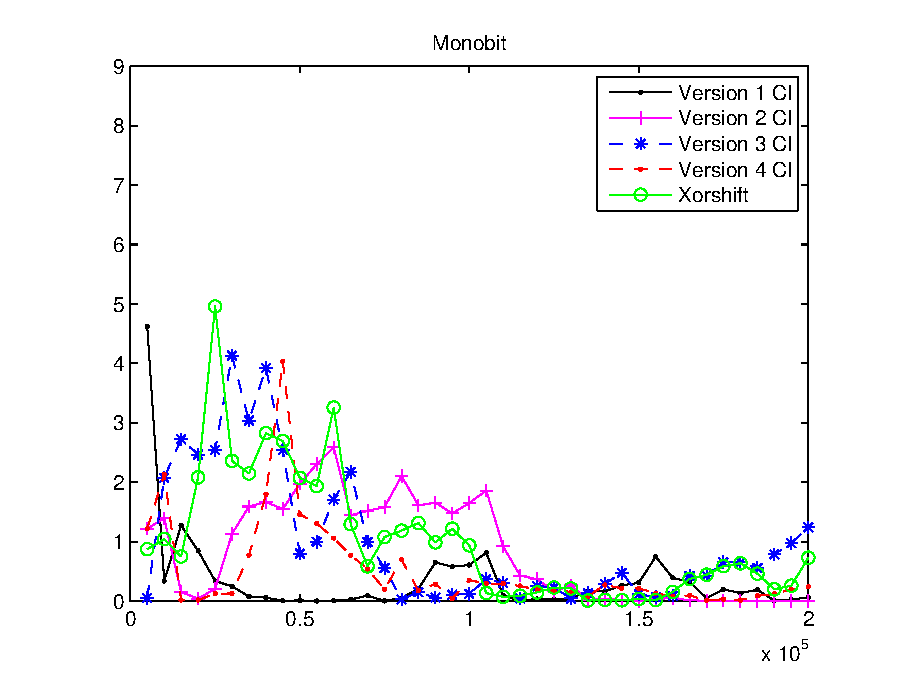
\includegraphics[scale=0.8]{monobits.eps}
% \includegraphics[width=3.7in]{4tests.eps}
\caption{Comparison of monobits tests}
\label{monobits}
\end{figure}

As a comparison of the overall stability of these PRNGs, similar tests have been computed for different sequence lengths (see Figures \ref{monobits} - \ref{autocorrelation}).
For the monobit test comparison (Figure \ref{monobits}), XORshift and Version 2-4 CI(XORshift, XORshift) PRNGs present the same values which are stable in a low level which never exceeds 1.2. Indeed, the new generators distributes very randomly the zeros and ones, whatever the length of the desired sequence. 
It can also be remarked that the XORshift generator presents the worst performance, but the values are within the standard boundary.
\begin{figure}
\centering
% \psfig{figure=2.eps,height=5in,width=3.5in}
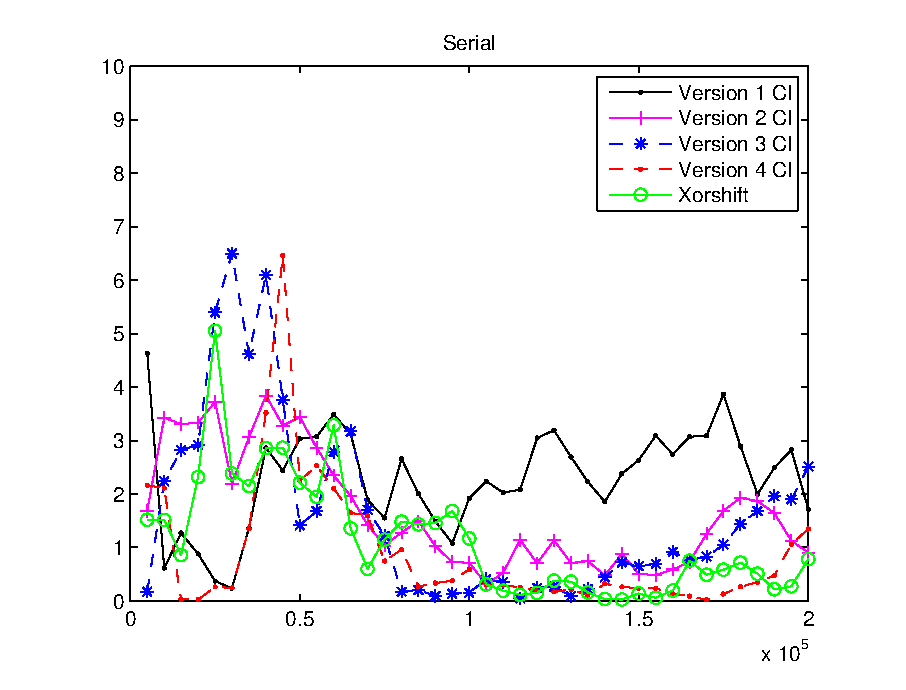
\includegraphics[scale=0.8]{serial.eps}
% \includegraphics[width=3.7in]{4tests.eps}
\caption{Comparison of serial tests}
\label{serial}
\end{figure}

Figure \ref{serial} shows the serial test comparison. The CI generators outputs perform this test, during the length of $2\times 10^4 to 5 \times 10^4$, Version 2 and 3 CI generators express a little overflow, except that all generators occurrences of 00, 01, 10, and 11 are very close to each other.

\begin{figure}
\centering
% \psfig{figure=2.eps,height=5in,width=3.5in}
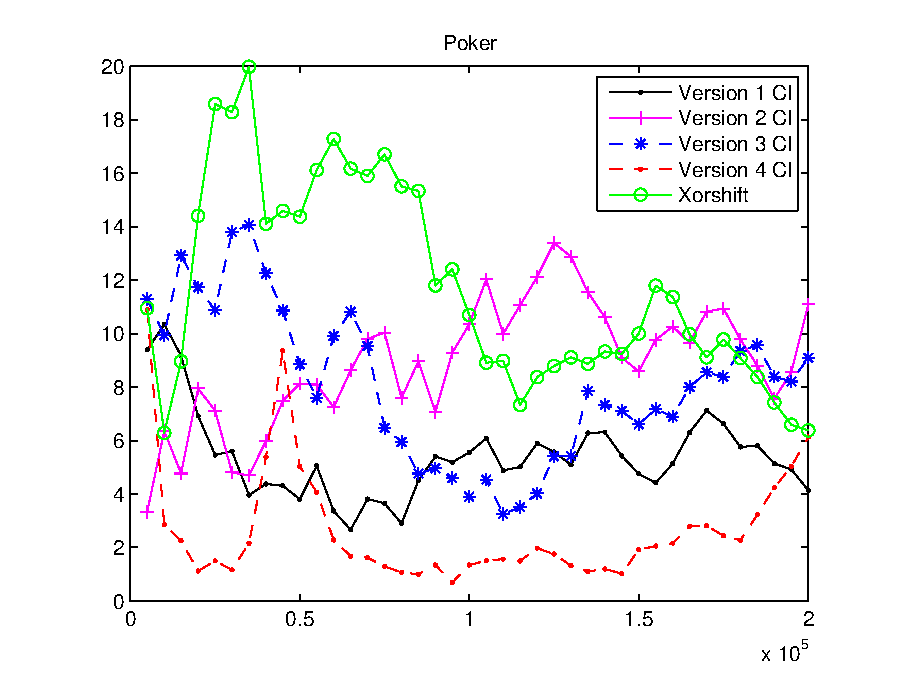
\includegraphics[scale=0.8]{poker.eps}
% \includegraphics[width=3.7in]{4tests.eps}
\caption{Comparison of poker tests}
\label{poker}
\end{figure}

The poker test comparison with $m=8$ is shown in Figure \ref{poker}. In some length, the XORshift is the not very stable generator in this tests. And our CI version generators are good that their value are slower than the threshold. 
%The reasons explaining this bad result can be, among other:
Indeed, the value of $m$ and the length of the sequences should be enlarged to be certain that the chaotic iterations express totally their complex behavior. In that situation, the performances of our generators in the poker test can be improved.
%but here we only achieve $2 \times 10^5$ sequence length, then m must be smaller than 13 to comply with the rule, if the sequence length is more, the performance of CI might be better.

\begin{figure}
\centering
% \psfig{figure=2.eps,height=5in,width=3.5in}
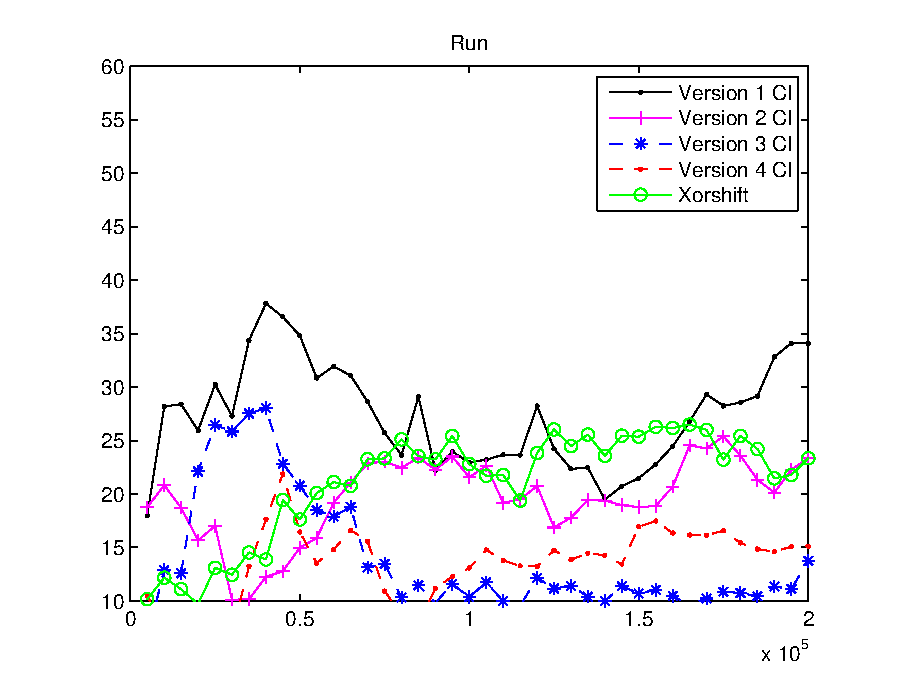
\includegraphics[scale=0.8]{runs.eps}
% \includegraphics[width=3.7in]{4tests.eps}
\caption{Comparison of runs tests}
\label{runs}
\end{figure}

The graph of the CI generators is the most stable one during the runs test comparison (Figure \ref{runs}). Moreover, this trend is reinforced when the lengths of the tested sequences are increased.


\begin{figure}
\centering
% \psfig{figure=2.eps,height=5in,width=3.5in}
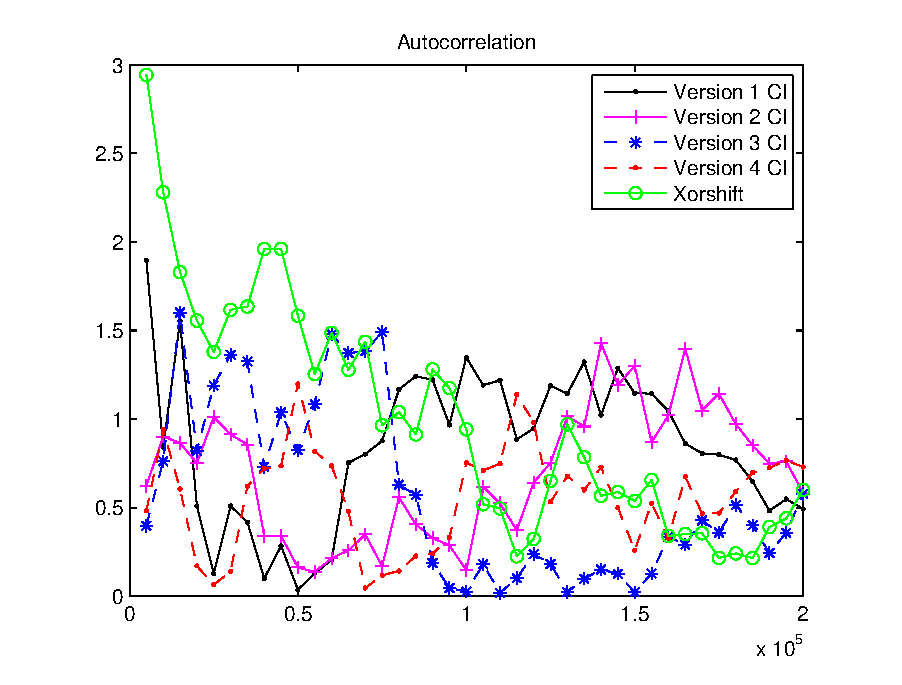
\includegraphics[scale=0.8]{autocorrelation1.eps}
% \includegraphics[width=3.7in]{4tests.eps}
\caption{Comparison of autocorrelation tests}
\label{autocorrelation}
\end{figure}


The comparison of autocorrelation tests is presented in Figure \ref{autocorrelation}. The CI generators clearly dominate these tests, whereas the score of the CI generators are all good.

To sum up we can claim that the CI generators, which newer version perform faster than its former version, outperforms all of the other generators in these statistical tests, especially when producing long output sequences.




\subsection{A flexible output}

We assume that the initial state $X$ is given as arrays of N-bit integers. Thus, the output size can be flexibly chosenell as $N$. Our PRNGs can generate discrete numbers
where the number of states could not match to a power of 2, which is suitable for stochastic differential equations as an example.(An attractive property of discrete random numbers is that they
require a small number of random bits--3 bits)~\cite{Ladd20092140}.
Moreover, due to the fact that CI process is a simple bitwise change, the speed of output integers and binary numbers is almost the same. 

In the following section, we will discuss the security level for various $N$ by Statistical test.
For both CI generator, various $N$ can pass all the NIST and DIEHARD test. Table~\ref{TestU01 Statistical Test} gives the results derived from applying the TestU01 battery of tests to the PRNGs considered in this work. As observed,an conclude that the effective range of $N$ for Version 2 CI is bigger than for Version 1 CI by TestU01. And also, this new scheme for obtaining a PRNG by combining two XORshift generators in CI give better properties than the old one (and the individual XORshift alone). It can be observed that the XORshift generator fails 146 tests.

\begin{table}[!t]
\begin{small}
\centering
\renewcommand{\arraystretch}{1.3}
\caption{TestU01 Statistical Test}
\label{TestU01 Statistical Test}
\centering
\begin{tabular}{cccccccccc}\toprule
\textbf{CI PRNG}&\textbf{Battery}&\textbf{N=2}&\textbf{N=4}&\textbf{N=8}&\textbf{N=16}&\textbf{N=32} \\\midrule

\multirow{7}*{\textbf{Version 1 CI}}&Rabbit	 	&2	&2	&2	&2	&3 \\
\multirow{7}*{\textbf{(XORshift,XORshift)}}&Alphabit 				&0	&0	&0	&2	&2 \\
&Pseudo DieHARD 								&0	&0	&0	&0	&0 \\
&FIPS\_140\_2 		 							&0	&0	&0	&0	&0 \\
&Small Crush 		 							&0	&0	&0	&1	&0 \\
&Crush 		 								&4	&4	&9	&16	&46 \\
&Big Crush 									&5	&3	&18	&30	&78 \\ 
\\
&Number of failures 	 							&11	&9	&29	&51	&129 \\
\bottomrule

\multirow{7}*{\textbf{Version 2 CI}}&Rabbit 					0	&0	&0	&0	&0 \\
\multirow{7}*{\textbf{(XORshift,XORshift)}}&Alphabit 				&4	&0	&0	&0	&0 \\
&Pseudo DieHARD 	 							&8	&2	&0	&0	&0 \\
&FIPS\_140\_2		 							&2	&0	&0	&0	&0 \\
&Small Crush 		 							&0	&0	&0	&0	&0 \\
&Crush 										&0	&0	&0	&0	&0 \\
&Big Crush 		 							&0	&0	&0	&0	&0 \\ 
\\
&Number of failures 	 							&14	&2	&0	&0	&0 \\
\bottomrule
\end{tabular}
\end{small}
\end{table}



\chapter{An optimization technique on pseudorandom generators based on chaotic iterations}
\minitoc
In this chapter, the statistical analysis of the three methods mentioned above are carried out systematically, and the results are discussed.
Indeed PRNGs are often based on modular arithmetic, logical operations like bitwise exclusive or (XOR), and on circular shifts of
bit vectors.
However the security level of some PRNGs of this kind has been revealed inadequate by today's standards.
Since different biased generators can possibly have their own side effects when inputted into our mixed generators, it is normal to enlarge the set of tested inputted PRNGs, to determine if the observed improvement still remains.
We will thus show in this research work that the intended statistical improvement is really effective for all of these most famous generators.



\section{About some Well-known PRNGs}
\label{The generation of pseudo-random sequence}

\subsection{Introduction}

Knowing that there is no universal generator, it is strongly recommended to test a stochastic application with a large set of different PRNGs~\cite{DavidRC2003643}. They can be classified in four major classes: linear generators, lagged generators, inversive generators, and mix generators:
\begin{itemize}
 \item \textbf{Linear generators}, defined by a linear recurrence, are the most commonly analyzed and utilized generators. The main linear generators are LCGs and MLCG.
 \item \textbf{Lagged generators} have a general recursive formula that use various previously computed terms in the determination of the new sequence value.
 \item \textbf{Inversive congruential generators} form a recent class of generators that are based on the principle of congruential inversion.
 \item \textbf{Mixed generators} result from the need for sequences of better and better quality, or at least longer periods. This has led to mix different types of PRNGs, as follows: $x^i=y^i\oplus z^i$
\end{itemize}


For instance, inversive generators are very interesting for verifying simulation results obtained with a linear congruential generator (LCG),
because their internal structure and correlation behavior strongly differs from what LCGs produce.
Since these generators have revealed several issues, some scientists refrain from using them.
In what follows, chaotic properties will be added to these PRNGs, leading to noticeable improvements observed by statistical test.
%Thus it helps scientists to enhance their habits by facilitating the use of sequences generated by generators that maybe they would not have used otherwise.
Let us firstly explain with more details the generators studied in this research work (for a synthetic view, see Fig.~\ref{Ontological class hierarchy of RNGs}).

\begin{figure}
\centering
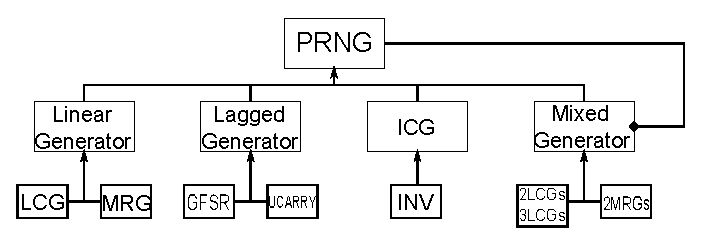
\includegraphics[width=3.5in]{TYPEPRNG.eps}
\DeclareGraphicsExtensions.
\caption{Ontological class hierarchy of PRNGs}
\label{Ontological class hierarchy of RNGs}
\end{figure}

\subsection{Details of some Existing Generators}

Here are the modules of PRNGs we have chosen to experiment.

\subsubsection{LCG}
This PRNG implements either the simple or the combined linear congruency generator (LCGs). The simple LCG is defined by the recurrence:
\begin{equation}
x^n = (ax^{n-1} + c)~mod~m
\label{LCG}
\end{equation}
where $a$, $c$, and $x^0$ must be, among other things, non-negative and less than $m$~\cite{Lecuyer2009}. In what follows, 2LCGs and 3LCGs refer as two (resp. three) combinations of such LCGs.
For further details, see~\cite{combined_lcg}.

\subsubsection{MRG}
This module implements multiple recursive generators (MRGs), based on a linear recurrence of order $k$, modulo $m$~\cite{Lecuyer2009}:
\begin{equation}
x^n = (a^1x^{n-1}+~...~+a^kx^{n-k})~mod~m
\label{MRG}
\end{equation}
Combination of two MRGs (referred as 2MRGs) is also be used in this paper.

\subsubsection{UCARRY}
Generators based on linear recurrences with carry are implemented in this module. This includes the add-with-carry (AWC) generator, based on the recurrence:
\begin{equation}
\label{AWC}
\begin{array}{l}
x^n = (x^{n-r} + x^{n-s} + c^{n-1})~mod~m, \\
c^n= (x^{n-r} + x^{n-s} + c^{n-1}) / m, \end{array}\end{equation}
the SWB generator, having the recurrence:
\begin{equation}
\label{SWB}
\begin{array}{l}
x^n = (x^{n-r} - x^{n-s} - c^{n-1})~mod~m, \\
c^n=\left\{
\begin{array}{l}
1 ~~~~~\text{if}~ (x^{i-r} - x^{i-s} - c^{i-1})<0\\
0 ~~~~~\text{else},\end{array} \right. \end{array}\end{equation}
%Implements the MWC generator:
%\begin{equation}
%\label{MWC}
%\begin{array}{l}
%x^n = (a^1x^{n-1} +~...~+a^rx^{n-r}+c^{n-1}) ~ mod ~ 2^w, \\
%c^n = (a^1x^{n-1} +~...~+a^rx^{n-r}+c^{n-1}) ~ /div ~ 2^w. \end{array}\end{equation}
and the SWC generator designed by R. Couture, which is based on the following recurrence:
\begin{equation}
\label{SWC}
\begin{array}{l}
x^n = (a^1x^{n-1} \oplus ~...~ \oplus a^rx^{n-r} \oplus c^{n-1}) ~ mod ~ 2^w, \\
c^n = (a^1x^{n-1} \oplus ~...~ \oplus a^rx^{n-r} \oplus c^{n-1}) ~ / ~ 2^w. \end{array}\end{equation}

\subsubsection{GFSR}
This module implements the generalized feedback shift register (GFSR) generator, that is:
\begin{equation}
x^n = x^{n-r} \oplus x^{n-k}
\label{GFSR}
\end{equation}

\subsubsection{INV}
Finally, this module implements the nonlinear inversive generator, as defined in~\cite{Lecuyer2009}, which is:

\begin{equation}
\label{INV}
\begin{array}{l}
x^n=\left\{
\begin{array}{ll}
(a^1 + a^2 / z^{n-1})~mod~m & \text{if}~ z^{n-1} \neq 0 \\
a^1 & \text{if}~  z^{n-1} = 0 .\end{array} \right. \end{array}\end{equation}


\section{statistical tests}
\label{Security analysis}

%A theoretical proof for the randomness of a generator is impossible to give, therefore statistical inference based on observed sample sequences produced by the generator seems to be the best option.
Considering the properties of binary random sequences, various statistical tests can be designed to evaluate the assertion that the sequence is generated by a perfectly random source. We have performed some statistical tests for the CIPRNGs proposed here. These tests include NIST suite~\cite{ANDREW2008} and DieHARD battery of tests~\cite{Marsaglia1996}. For completeness and for reference, we give in the following subsection a brief description of each of the aforementioned tests.

\subsection{NIST statistical tests suite}

Among the numerous standard tests for pseudo-randomness, a convincing way to show the randomness of the produced sequences is to confront them to the NIST (National Institute of  Standards and Technology) statistical tests, being an up-to-date tests suite proposed by the Information Technology Laboratory (ITL). A new version of the Statistical tests suite has been released in August 11, 2010.

The NIST tests suite SP 800-22 is a statistical package consisting of 15 tests. They were developed to test the randomness of binary sequences produced by hardware or software based cryptographic pseudorandom number generators. These tests focus on a variety of different types of non-randomness that could exist in a sequence.

For each statistical test, a set of $P-values$ (corresponding to the set of sequences) is produced.
The interpretation of empirical results can be conducted in various ways.
In this paper, the examination of the distribution of P-values to check for uniformity ($ P-value_{T}$) is used.
The distribution of $P-values$ is examined to ensure uniformity.
If $P-value_{T} \geqslant 0.0001$, then the sequences can be considered to be uniformly distributed.

In our experiments, 100 sequences (s = 100), each with 1,000,000-bit long, are generated and tested. If the $P-value_{T}$ of any test is smaller than 0.0001, the sequences are considered to be not good enough and the generating algorithm is not suitable for usage.





\subsection{DieHARD battery of tests}
The DieHARD battery of tests has been the most sophisticated standard for over a decade. Because of the stringent requirements in the DieHARD tests suite, a generator passing this battery of
tests can be considered good as a rule of thumb.

The DieHARD battery of tests consists of 18 different independent statistical tests. This collection
 of tests is based on assessing the randomness of bits comprising 32-bit integers obtained from
a random number generator. Each test requires $2^{23}$ 32-bit integers in order to run the full set
of tests. Most of the tests in DieHARD return a $P-value$, which should be uniform on $[0,1)$ if the input file
contains truly independent random bits.  These $P-values$ are obtained by
$P=F(X)$, where $F$ is the assumed distribution of the sample random variable $X$ (often normal).
But that assumed $F$ is just an asymptotic approximation, for which the fit will be worst
in the tails. Thus occasional $P-values$ near 0 or 1, such as 0.0012 or 0.9983, can occur.
An individual test is considered to be failed if the $P-value$ approaches 1 closely, for example $P>0.9999$.

\section{Results and discussion}
\label{Results and discussion}


\begin{sidewaystable}
\caption{NIST and DieHARD tests suite passing rates for PRNGs without CI}
\label{NIST and DieHARD tests suite passing rate the for PRNGs without CI}
\centering
\begin{tabular}{|l||c|c|c|c|c|c|c|c|c|c|}
    \hline\hline
Types of PRNGs & \multicolumn{2}{c|}{Linear PRNGs} & \multicolumn{4}{c|}{Lagged PRNGs} & \multicolumn{1}{c|}{ICG PRNGs} & \multicolumn{3}{c|}{Mixed PRNGs}\\ \hline
\backslashbox{\textbf{$Tests$}} {\textbf{$PRNG$}} & LCG& MRG& AWC & SWB  & SWC & GFSR & INV & LCG2& LCG3& MRG2 \\ \hline
NIST & 11/15 & 14/15 &\textbf{15/15} & \textbf{15/15}   & 14/15 & 14/15  & 14/15 & 14/15& 14/15& 14/15 \\ \hline
DieHARD & 16/18 & 16/18 & 15/18 & 16/18 & \textbf{18/18} & 16/18 & 16/18 & 16/18& 16/18& 16/18\\ \hline
\end{tabular}
\end{sidewaystable}



Table~\ref{NIST and DieHARD tests suite passing rate the for PRNGs without CI} shows the results on the batteries recalled above, indicating that almost all the PRNGs cannot pass all their tests. In other words, the statistical quality of these PRNGs cannot fulfill the up-to-date standards presented previously. We will show that the CIPRNG can solve this issue.

To illustrate the effects of this CIPRNG in detail, experiments will be divided in three parts:
\begin{enumerate}
  \item \textbf{Single CIPRNG}: The PRNGs involved in CI computing are of the same category.
  \item \textbf{Mixed CIPRNG}: Two different types of PRNGs are mixed during the chaotic iterations process.
  \item \textbf{Multiple CIPRNG}: The generator is obtained by repeating the composition of the iteration function as follows: $x^0\in \mathds{B}^{\mathsf{N}}$, and $\forall n\in \mathds{N}^{\ast },\forall i\in \llbracket1;\mathsf{N}\rrbracket,$
\begin{equation}
\begin{array}{l}
x_i^n=\left\{
\begin{array}{l}
x_i^{n-1}~~~~~\text{if}~S^n\neq i \\
\forall j\in \llbracket1;\mathsf{m}\rrbracket,f^m(x^{n-1})_{S^{nm+j}}~\text{if}~S^{nm+j}=i.\end{array} \right. \end{array}
\end{equation}
$m$ is called the \emph{functional power}.
\end{enumerate}


We have performed statistical analysis of each of the aforementioned CIPRNGs.
The results are reproduced in Tables~\ref{NIST and DieHARD tests suite passing rate the for PRNGs without CI} and \ref{NIST and DieHARD tests suite passing rate the for single CIPRNGs}.
The scores written in boldface indicate that all the tests have been passed successfully, whereas an asterisk ``*'' means that the considered passing rate has been improved.
\subsection{Tests based on the Single CIPRNG}

\begin{sidewaystable}
\renewcommand{\arraystretch}{1.3}
\caption{NIST and DieHARD tests suite passing rates for PRNGs with CI}
\label{NIST and DieHARD tests suite passing rate the for single CIPRNGs}
\centering
  \begin{tabular}{|l||c|c|c|c|c|c|c|c|c|c|c|c|}
    \hline
Types of PRNGs & \multicolumn{2}{c|}{Linear PRNGs} & \multicolumn{4}{c|}{Lagged PRNGs} & \multicolumn{1}{c|}{ICG PRNGs} & \multicolumn{3}{c|}{Mixed PRNGs}\\ \hline
\backslashbox{\textbf{$Tests$}} {\textbf{$Single~CIPRNG$}} & LCG  & MRG & AWC & SWB & SWC & GFSR & INV& LCG2 & LCG3& MRG2 \\ \hline\hline
Old CIPRNG\\ \hline \hline
NIST & \textbf{15/15} *  & \textbf{15/15} * & \textbf{15/15}   & \textbf{15/15}   & \textbf{15/15} * & \textbf{15/15} * & \textbf{15/15} *& \textbf{15/15} * & \textbf{15/15} * & \textbf{15/15} \\ \hline
DieHARD & \textbf{18/18} *  & \textbf{18/18} * & \textbf{18/18} *  & \textbf{18/18} *  & \textbf{18/18}  & \textbf{18/18} * & \textbf{18/18} *& \textbf{18/18} * & \textbf{18/18} *& \textbf{18/18} * \\ \hline
New CIPRNG\\ \hline \hline
NIST & \textbf{15/15} *  & \textbf{15/15} * & \textbf{15/15}   & \textbf{15/15}  & \textbf{15/15} * & \textbf{15/15} * & \textbf{15/15} *& \textbf{15/15} * & \textbf{15/15} * & \textbf{15/15} \\ \hline
DieHARD & \textbf{18/18} *  & \textbf{18/18} * & \textbf{18/18} * & \textbf{18/18} * & \textbf{18/18}  & \textbf{18/18} * & \textbf{18/18} * & \textbf{18/18} * & \textbf{18/18} *& \textbf{18/18} *\\ \hline
Xor CIPRNG\\ \hline\hline
NIST & 14/15*& \textbf{15/15} *   & \textbf{15/15}   & \textbf{15/15}   & 14/15 & \textbf{15/15} * & 14/15& \textbf{15/15} * & \textbf{15/15} *& \textbf{15/15}  \\ \hline
DieHARD & 16/18 & 16/18 & 17/18* & \textbf{18/18} * & \textbf{18/18}  & \textbf{18/18} * & 16/18 & 16/18 & 16/18& 16/18\\ \hline
\end{tabular}
\end{sidewaystable}

The statistical tests results of the PRNGs using the single CIPRNG method are given in Table~\ref{NIST and DieHARD tests suite passing rate the for single CIPRNGs}.
We can observe that, except for the Xor CIPRNG, all of the CIPRNGs have passed the 15 tests of the NIST battery and the 18 tests of the DieHARD one.
Moreover, considering these scores, we can deduce that both the single Old CIPRNG and the single New CIPRNG are relatively steadier than the single Xor CIPRNG approach, when applying them to different PRNGs.
However, the Xor CIPRNG is obviously the fastest approach to generate a CI random sequence, and it still improves the statistical properties relative to each generator taken alone, although the test values are not as good as desired.

Therefore, all of these three ways are interesting, for different reasons, in the production of pseudorandom numbers and,
on the whole, the single CIPRNG method can be considered to adapt to or improve all kinds of PRNGs.

To have a realization of the Xor CIPRNG that can pass all the tests embedded into the NIST battery, the Xor CIPRNG with multiple functional powers are investigated in Section~\ref{Tests based on Multiple CIPRNG}.



\subsection{Tests based on the Mixed CIPRNG}

To compare the previous approach with the CIPRNG design that uses a Mixed CIPRNG, we have taken into account the same inputted generators than in the previous section.
These inputted couples $(PRNG_1,PRNG_2)$ of PRNGs are used in the Mixed approach as follows:
\begin{equation}
\left\{
\begin{array}{l}
x^0 \in \llbracket 0, 2^\mathsf{N}-1 \rrbracket, S \in \llbracket 0, 2^\mathsf{N}-1 \rrbracket^\mathds{N} \\
\forall n \in \mathds{N}^*, x^n = x^{n-1} \oplus PRNG_1\oplus PRNG_2,
\end{array}
\right.
\label{equation Oplus}
\end{equation}

With this Mixed CIPRNG approach, both the Old CIPRNG and New CIPRNG continue to pass all the NIST and DieHARD suites.
In addition, we can see that the PRNGs using a Xor CIPRNG approach can pass more tests than previously.
The main reason of this success is that the Mixed Xor CIPRNG has a longer period.
Indeed, let $n_{P}$ be the period of a PRNG $P$, then the period deduced from the single Xor CIPRNG approach is obviously equal to:
\begin{equation}
n_{SXORCI}=
\left\{
\begin{array}{ll}
n_{P}&\text{if~}x^0=x^{n_{P}}\\
2n_{P}&\text{if~}x^0\neq x^{n_{P}}.\\
\end{array}
\right.
\label{equation Oplus}
\end{equation}

Let us now denote by $n_{P1}$ and $n_{P2}$ the periods of respectively the $PRNG_1$ and $PRNG_2$ generators, then the period of the Mixed Xor CIPRNG will be:
\begin{equation}
n_{XXORCI}=
\left\{
\begin{array}{ll}
LCM(n_{P1},n_{P2})&\text{if~}x^0=x^{LCM(n_{P1},n_{P2})}\\
2LCM(n_{P1},n_{P2})&\text{if~}x^0\neq x^{LCM(n_{P1},n_{P2})}.\\
\end{array}
\right.
\label{equation Oplus}
\end{equation}

In Table~\ref{DieHARD fail mixex CIPRNG}, we only show the results for the Mixed CIPRNGs that cannot pass all DieHARD suites (the NIST tests are all passed). It demonstrates that Mixed Xor CIPRNG involving LCG, MRG, LCG2, LCG3, MRG2, or INV cannot pass the two following tests, namely the ``Matrix Rank 32x32'' and the ``COUNT-THE-1's'' tests contained into the DieHARD battery. Let us recall their definitions:

\begin{itemize}
 \item \textbf{Matrix Rank 32x32.} A random 32x32 binary matrix is formed, each row having a 32-bit random vector. Its rank is an integer that ranges from 0 to 32. Ranks less than 29 must be rare, and their occurences must be pooled with those of rank 29. To achieve the test, ranks of 40,000 such random matrices are obtained, and a chisquare test is performed on counts for ranks 32,31,30 and for ranks $\leq29$.

 \item \textbf{COUNT-THE-1's TEST} Consider the file under test as a stream of bytes (four per  2 bit integer).  Each byte can contain from 0 to 8 1's, with probabilities 1,8,28,56,70,56,28,8,1 over 256.  Now let the stream of bytes provide a string of overlapping  5-letter words, each ``letter'' taking values A,B,C,D,E. The letters are determined by the number of 1's in a byte: 0,1, or 2 yield A, 3 yields B, 4 yields C, 5 yields D and 6,7, or 8 yield E. Thus we have a monkey at a typewriter hitting five keys with various probabilities (37,56,70,56,37 over 256).  There are $5^5$ possible 5-letter words, and from a string of 256,000 (over-lapping) 5-letter words, counts are made on the frequencies for each word.   The quadratic form in the weak inverse of the covariance matrix of the cell counts provides a chisquare test: Q5-Q4, the difference of the naive Pearson sums of $(OBS-EXP)^2/EXP$ on counts for 5- and 4-letter cell counts.
\end{itemize}

The reason of these fails is that the output of LCG, LCG2, LCG3, MRG, and MRG2 under the experiments are in 31-bit. Compare with the Single CIPRNG, using different PRNGs to build CIPRNG seems more efficient in improving random number quality (mixed Xor CI can 100\% pass NIST, but single cannot).

\begin{table*}
\renewcommand{\arraystretch}{1.3}
\caption{Scores of mixed Xor CIPRNGs when considering the DieHARD battery}
\label{DieHARD fail mixex CIPRNG}
\centering
  \begin{tabular}{|l||c|c|c|c|c|c|}
    \hline
\backslashbox{\textbf{$PRNG_1$}} {\textbf{$PRNG_0$}} & LCG & MRG & INV & LCG2 & LCG3 & MRG2 \\ \hline\hline
LCG  &\backslashbox{} {} &16/18&16/18 &16/18 &16/18 &16/18\\ \hline
MRG &16/18 &\backslashbox{} {} &16/18&16/18 &16/18  &16/18\\ \hline
INV &16/18 &16/18&\backslashbox{} {} &16/18 &16/18&16/18    \\ \hline
LCG2  &16/18 &16/18 &16/18 &\backslashbox{} {}  &16/18&16/18\\ \hline
LCG3  &16/18 &16/18 &16/18&16/18&\backslashbox{} {} &16/18\\ \hline
MRG2 &16/18  &16/18 &16/18&16/18 &16/18 &\backslashbox{} {}  \\ \hline
\end{tabular}
\end{table*}

\subsection{Tests based on the Multiple CIPRNG}
\label{Tests based on Multiple CIPRNG}

Until now, the combination of at most two input PRNGs has been investigated.
We now regard the possibility to use a larger number of generators to improve the statistics 
of the generated pseudorandom numbers, leading to the multiple functional power approach.
For the CIPRNGs which have already pass both the NIST and DieHARD suites with 2 inputted PRNGs 
(all the Old and New CIPRNGs, and some of the Xor CIPRNGs), it is not meaningful to consider 
their adaption of this multiple CIPRNG method, hence only the Multiple Xor CIPRNGs, 
having the following form, will be investigated.
\begin{equation}
\left\{
\begin{array}{l}
x^0 \in \llbracket 0, 2^\mathsf{N}-1 \rrbracket, S \in \llbracket 0, 2^\mathsf{N}-1 \rrbracket^\mathds{N} \\
\forall n \in \mathds{N}^*, x^n = x^{n-1} \oplus S^{nm}\oplus S^{nm+1}\ldots \oplus S^{nm+m-1} ,
\end{array}
\right.
\label{equation Oplus}
\end{equation}

The question is now to determine the value of the threshold $m$ (the functional power) making 
the multiple CIPRNG being able to pass the whole NIST battery.
Such a question is answered in Table~\ref{threshold}.


\begin{table*}
\renewcommand{\arraystretch}{1.3}
\caption{Functional power $m$ making it possible to pass the whole NIST battery}
\label{threshold}
\centering
  \begin{tabular}{|l||c|c|c|c|c|c|c|c|}
    \hline
Inputted $PRNG$ & LCG & MRG & SWC & GFSR & INV& LCG2 & LCG3  & MRG2 \\ \hline\hline
Threshold  value $m$& 19 & 7  & 2& 1 & 11& 9& 3& 4\\ \hline\hline
\end{tabular}
\end{table*}

\subsection{Results Summary}

We can summarize the obtained results as follows.
\begin{enumerate}
\item The CIPRNG method is able to improve the statistical properties of a large variety of PRNGs.
\item Using different PRNGs in the CIPRNG approach is better than considering several instances of one unique PRNG.
\item The statistical quality of the outputs increases with the functional power $m$.
\end{enumerate}

In this chapter, we first have formalized the CI methods that has been already presented in previous Internet conferences.
These CI methods are based on iterations that have been topologically proven as chaotic.
Then 10 usual PRNGs covering all kinds of generators have been applied, and the NIST and DieHARD batteries have been tested.
Analyses show that PRNGs using the CIPRNG methods do not only inherit the chaotic properties of the
CI iterations, they also have improvements of their statistics.
This is why CIPRNG techniques should be considered as post-treatments on pseudorandom number generators to improve both their randomness and security.


\chapter{FPGA Acceleration of CIPRNGs}
In this chapter, the proposition is to improve widely the efficient of the formerly proposed generators, without any lack of chaos properties. To do that, Field programmable gate array (FPGA) method is proposed.

\section{introduction}
Nowadays, FPGAs are very successfully applied to implement random sequence generation due to its ability in highly parallelizable task \cite{Bojani200663, Danger:2009:HST:1645457.1645933, Tsoi:2003:CFT:938383.938400}. Such device allows us to generate pseudorandom numbers with remarkable speed. In these and other implementations, FPGA has advantages in performance, design time, power consumption, flexibility, cost and so on.

According to the previous chapters' description, it has proven that the chaotic iterations (CIs), to be a very decent tool for computing iterative algorithms, satisfies the chaos property, as it is defined by Devaney. The chaotic behaviour of CIs is developed attempt to obtain an unpredictable PRNG, in \cite{DBLP:journals/corr/abs-1112-5239}, its efficient implementations on GPU have been designed in, expressing that a very large quantity of pseudorandom numbers can be generated per second. Here, generators based on chaotic iteration is designed specifically for FPGA hardware, with that, the rate of generation can be hugely increased.

\section{FPGA design}
\label{FPGA design}
In order to take benefits from the computing power of FPGA, a whole processing needs to spread into several independent blocks  of threads that can be computed simultaneously. In general,  the larger the number of  threads is, the more logistic elements of FPGA are used, and the less branching  instructions are used  (if,  while,  ...),  the  better the  performances  on  FPGA  is. Obviously, having these requirements in  mind, suitable CIPRNG algorithms which produce random numbers with chaotic properties should be chosen to apply to FPGA. The Verilog-HDL~\cite{verilog} is used to help program. 

\subsection{CI Version selection}
According to the comparison in Chapter~\ref{Statistical Tests for Randomness}, it can be seen that Version 4 CI algorithms is the most adaptable of all, its loop processing of them are both able to be replaced by parallel computing to increase the efficiency. To be noticed, the CIPRNGs used here are both proven to be cryptographically secure (check Section~\ref{Security Analysis}) by using BBS and three XORshift PRNGs, and its statistical performance is withstand the TestU01 test suite (Section~\ref{test for Version 4 CI}).
\subsection{Design of XORshift}
The structure of PRNG XORshift designed in Verilog-HDL is shown in Figure
\ref{xorshift verilog}, there are four inputs, first one is the initial state, which cost 64 bits 
of register units, then the other three ones are used to define how to shift, in FPGA, shifting cost no 
elements (just using different bit cell of the input). Then there are $64 - s1 + 64 -s2 + 64 -s3 
= 192 - s1 - s2 - s3$ logic gates elements applied for XORshift processing. In program, we define 
each FPGA clock positive edge, the XORshift will work, since these are simple processing for FPGA, every 
clock step can lead to one output.
\begin{figure}
\begin{center}
  \subfigure[XORshift]{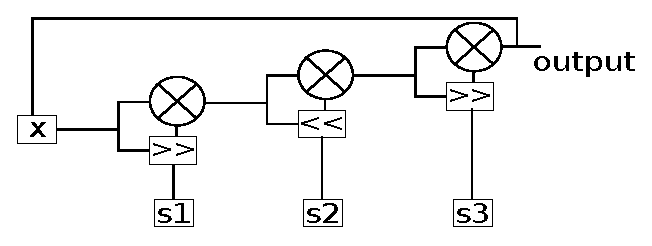
\includegraphics[width=6.5cm]{xorshift.eps}
  \label{xorshift verilog}}
  \subfigure[BBS]{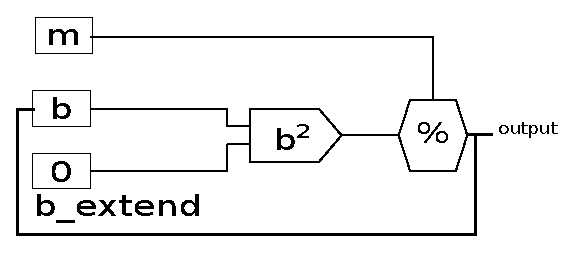
\includegraphics[width=6.5cm]{bbs.eps}
  \label{BBS verilog}}
\end{center}
\caption{The structure of processing for XORshift and BBS in FPGA each clock step}
\end{figure}

\subsection{Design of BBS}
Figure~\ref{BBS verilog} gives the design of BBS in FPGA, there are two $32$ bits length input: 
$b$ and $m$, $m$ is also a register stores the value of M which will not be changed, register $b$ 
stores the every time state, when it is processing square computation, another register $b\_extend$ 
is used to combine with $b$ to a $64$ bits length data to avoid overflow. At last output is taking 
the three LSBs from the output of $\%$ as output. BBS performs the function while every positive 
edge of clock.

\subsection{Design of the Version 4 CI}
For composition of the CI PRNG, two XORshifts and BBS are connected to work together (Figure~\ref{CI verilog}), 
as shown, the three bits of the output of BBS are the switches for the corresponding $32$ bits from 
XORshift outputs. Every round of the CI RPNG processing costs two times clock positive edge to finish: In first clock, 
the four PRNGs are processed in parallel; Then in second clock, the results of the classic PRNGs are combined with 
the state to produce the output ($32$ bits binary).


\begin{figure}
 \begin{center}
 
  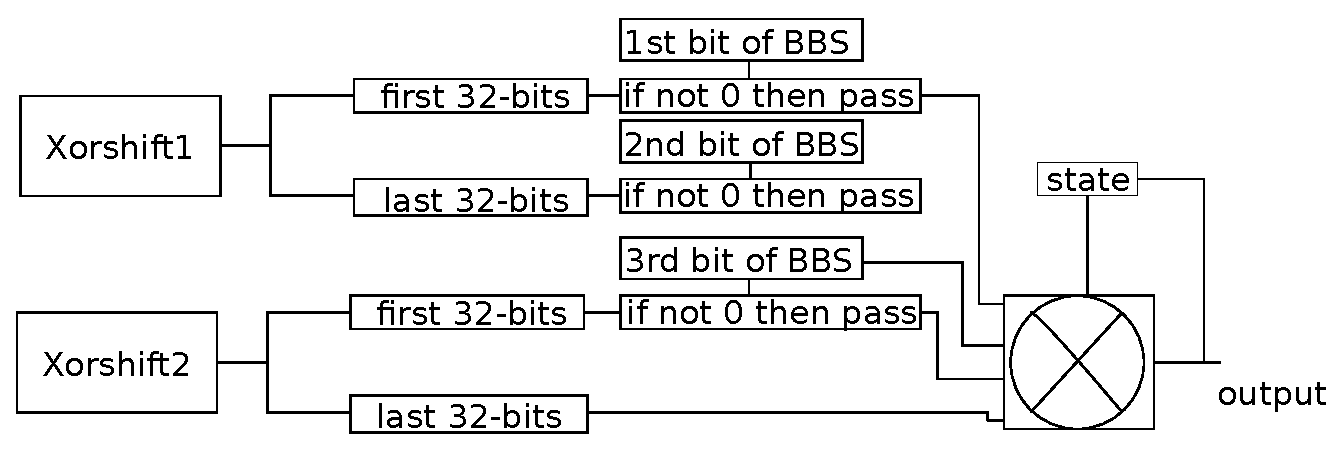
\includegraphics[width=10cm]{ci.eps}
  \label{CI verilog}
  \caption{The structure of CI PRNG in FPGA}
 \end{center}
\end{figure}

In our experiment, type $EP2C8Q208C8$ from Altera 
company's CYCLONE II FPGA series is applied, it can 
give $50$ MHz working clock frequency in default,
with the help of phase-lock loop (PLL) device, the frequency could be increased into 
$400$ MHz,then our generator based on CI can achieve $400 (MHz) \div 2 (times) \times 32 (bits)$
which can achieve about $6400$ Mbits per second, and there are 100 logic elements used totally, 
that only takes $1\%$ in $EP2C8Q208C8$ ($100$ from $8256$ logic elements shown in 
Figure~\ref{logic elements}). 
In next section, an information hiding 
application is expressed by the FPGA device.

\begin{figure}
\begin{center}
  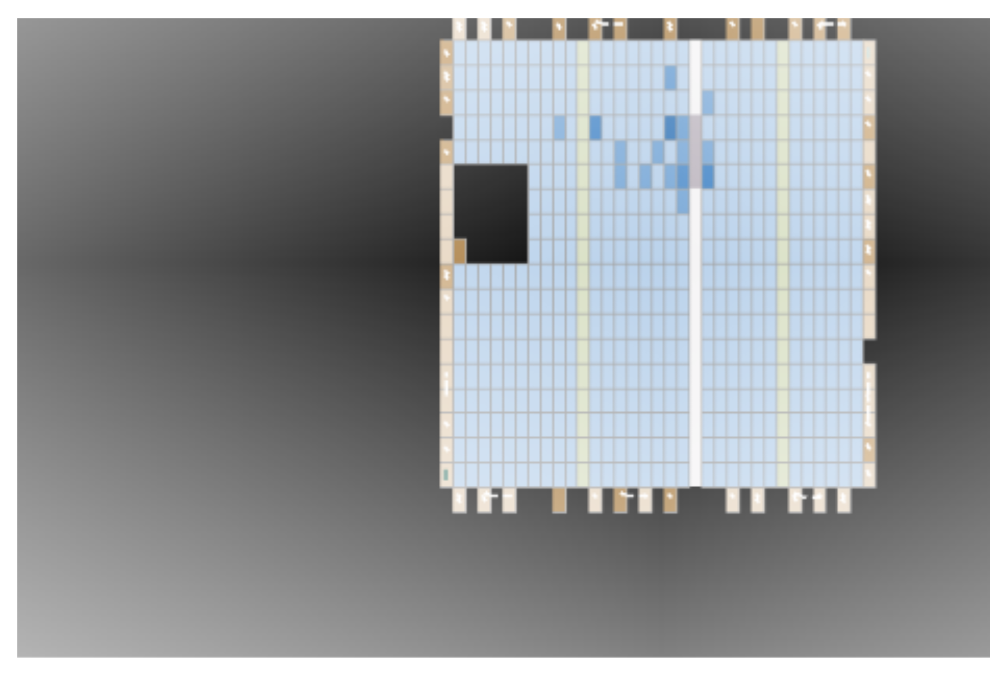
\includegraphics[width=6.5cm]{print.eps}
\end{center}
\caption{The sources cost in $EP2C8Q208C8$ FPGA board}
 \label{logic elements}
\end{figure}


\chapter{Applications in cryptology}
\label{Application Example}
\minitoc

\section{Application example of the use of the proposed PRNG}
\label{An application example of the proposed PRNG}

Cryptographically secure PRNGs are fundamental tools to communicate through the Internet. Original and encrypted image are shown in Figures~\ref{Distribution of original image}(a) and 
~\ref{Distribution of encrypted image}(a), whereas Figure~\ref{Distribution of original image}(b) and ~\ref{Distribution of encrypted image}(b) depict their histograms. 
Obviously the distribution of the encrypted image is very close to the uniform distribution, which improves the protection against statistical attacks.





\begin{figure*}
\begin{minipage}[b]{.48\linewidth}
\centering
\centerline{\epsfig{figure=lena.eps,width=5cm}}
\centerline{(a) Original image.}
\end{minipage}
\hfill
\begin{minipage}[b]{0.48\linewidth}
\centering
\centerline{\epsfig{figure=Histogram_lena.eps,width=8cm}}
\centerline{(b) Histogram.}
\end{minipage}
\caption{Distribution of original image}
\label{Distribution of original image}
\end{figure*}

\begin{figure*}
\begin{minipage}[b]{.48\linewidth}
\centering
\centerline{\epsfig{figure=lena_crypt.eps,width=5cm}}
\centerline{(a) Encrypted image.}
\end{minipage}
\hfill
\begin{minipage}[b]{0.48\linewidth}
\centering
\centerline{\epsfig{figure=Histogram_lena_crypt.eps,width=8cm}}
\centerline{(b) Histogram.}
\end{minipage}
\caption{Distribution of encrypted image}
\label{Distribution of encrypted image}
\end{figure*}

Figure~\ref{Correlation distributions of two horizontally adjacent pixels in the original image and the encrypted image} shows the correlation distribution of two horizontally adjacent pixels, both in the original and in the encrypted images. Correlation coefficients in the horizontal, vertical, and diagonal directions concerning these two images are presented in Table~\ref{Correlation coefficients of two adjacent pixels in the original image and the encrypted image}. Obviously, the correlation is important in the original image, whereas it is low and can be ignored in the encrypted image. These simple illustrations tend to prove that the use of CI PRNGs for cryptographic applications can be studied, to determine whether these chaotic generators is cryptographically secure working at the application or not. These study has been partially initiated in \cite{guyeuxTaiwan10,bgw10:ip,bfgw11:ij,bfg12b:ip}, in which our generators have been used as a component of watermarking scheme. The robustness of this scheme 
has been evaluated, which has led to results as good as possible, thus reinforcing our opinion that these generators would probably be useful in cryptographic applications.
The question of whether CI PRNGs are working application well or not, will thus be raised in our next work.

\begin{figure*}
\begin{minipage}[b]{.48\linewidth}
\centering
\centerline{\epsfig{figure=Correlation_distribution_of_the_original_image.eps,width=8cm}}
\centerline{(a) Original image.}
\end{minipage}
\hfill
\begin{minipage}[b]{0.48\linewidth}
\centering
\centerline{\epsfig{figure=Correlation_distribution_of_the_encrypted_image.eps,width=8cm}}
\centerline{(b) Encrypted image.}
\end{minipage}
\caption{Correlation distributions of two horizontally adjacent pixels}
\label{Correlation distributions of two horizontally adjacent pixels in the original image and the encrypted image}
\end{figure*}

\begin{table*}
\renewcommand{\arraystretch}{1.3}
\caption{Correlation coefficients of two adjacent pixels in the original image and the encrypted image}
\label{Correlation coefficients of two adjacent pixels in the original image and the encrypted image}
\centering
\begin{tabular}{ccc} \toprule
\textbf{Direction} &\textbf{Original image} & \textbf{Encrypted image} \\ \midrule
Horizontal &0.9245 &-0.0059 \\
Vertical &0.9617 &-0.0048 \\
Diagonal &0.8967 &-0.0052 \\ \bottomrule
\end{tabular}
\end{table*}


\section{Introduction}

Information hiding is now an integral part of Internet technologies. In the field of social search engines, for example, contents like pictures or movies are tagged with descriptive labels by contributors, and search results are determined by these descriptions. These collaborative taggings, used for example in Flickr~\cite{Frick} and Delicious~\cite{Delicious} websites, contribute to the development of a Semantic Web, in which every Web page contains machine-readable metadata that describe its content. Information hiding technologies can be used for embedding these metadata. The advantage of its use is the possibility to realize  social search without websites and databases: descriptions are directly embedded into media, whatever their formats. Robustness is required in this situation, as descriptions should resist to modifications like resizing, compression, and format conversion.

The Internet security field is also concerned by watermarking technologies. Steganography and cryptography are supposed to be used by terrorists to communicate through the Internet. Furthermore, in the areas of defense or in industrial espionage, many information leaks using steganographic techniques have been discovered. Lastly, watermarking is often cited as a possible solution to digital rights managements issues, to counteract piracy of digital work in an Internet based entertainment world~\cite{Nakashima2003}.

\section{Definition of a Chaos-Based Information Hiding Scheme}
\label{sec:Algo}

Let us now introduce our information hiding scheme based on CI generators.


\subsection{Most and least significant coefficients}

Let us define the notions of most and least significant coefficients of an image.

\begin{Definition}
\label{definitionMSC}
For a given image, most significant coefficients (in short MSCs), are coefficients that allow the description of the relevant part of the image, \emph{i.e.}, its richest part (in terms of embedding information), through a sequence of bits.
\end{Definition}

For example, in a spatial description of a grayscale image, a definition of MSCs can be the sequence constituted by the first four bits of each pixel (see Figure~\ref{fig:MSCLC}). In a discrete cosine frequency domain description, each $8\times 8$ block of the carrier image is mapped onto a list of 64 coefficients. The energy of the image is mostly contained in a determined part of themselves, which can constitute a possible sequence of MSCs.

\begin{Definition}
\label{definitionLSC}
By least significant coefficients (LSCs), we mean a translation of some insignificant parts of a medium in a sequence of bits (insignificant can be understand as: ``which can be altered without sensitive damages'').
\end{Definition}

These LSCs can be, for example, the last three bits of the gray level of each pixel (see Figure~\ref{fig:MSCLC}). Discrete cosine, Fourier, and wavelet transforms can be used also to generate LSCs and MSCs. Moreover, these definitions can be extended to other types of media.




\begin{figure}[htb]

\begin{minipage}[b]{1.0\linewidth}
  \centering
 \centerline{\epsfig{figure=lena512.eps,width=4cm}}
  \centerline{(a) Lena.}
\end{minipage}

\begin{minipage}[b]{.48\linewidth}
  \centering
 \centerline{\epsfig{figure=lena_msb_678.eps,width=4cm}}
  \centerline{(b) MSCs of Lena.}
\end{minipage}
\hfill
\begin{minipage}[b]{0.48\linewidth}
  \centering
 \centerline{\epsfig{figure=lena_lsb_1234_facteur17.eps,width=4cm}}
  \centerline{(c) LSCs of Lena ($\times 17$).}
\end{minipage}
%
\caption{Example of most and least significant coefficients of Lena.}
\label{fig:MSCLC}
%
\end{figure}


LSCs are used during the embedding stage. Indeed, some of the least significant coefficients of the carrier image will be chaotically chosen by using our PRNG. These bits will be either switched or replaced by the bits of the watermark. The MSCs are only useful in case of authentication; mixture and embedding stages depend on them. Hence, a coefficient should not be defined at the same time as a MSC and a LSC: the last can be altered while the first is needed to extract the watermark.

\subsection{Stages of the scheme}

Our CI generator-based information hiding scheme consists of two stages: (1) mixture of the watermark and (2) its embedding.

\subsubsection{Watermark mixture}
Firstly, for security reasons, the watermark can be mixed before its embedding into the image. A first way to achieve this stage is to apply the bitwise exclusive or (XOR) between the watermark and the CI generator. In this paper, we introduce a new mixture scheme based on chaotic iterations. Its chaotic strategy, which depends on our PRNG, will be highly sensitive to the MSCs, in the case of an authenticated watermarking.

\subsubsection{Watermark embedding}
Some LSCs will be switched, or substituted by the bits of the possibly mixed watermark. To choose the sequence of LSCs to be altered, a number of integers, less than or equal to the number $\mathsf{M}$ of LSCs corresponding to a chaotic sequence $U$, is generated from the chaotic strategy used in the mixture stage. Thus, the $U^{k}$-th least significant coefficient of the carrier image is either switched, or substituted by the $k^{th}$ bit of the possibly mixed watermark. In case of authentication, such a procedure leads to a choice of the LSCs which are highly dependent on the MSCs~\cite{guyeux10}.

On the one hand, when the switch is chosen, the watermarked image is obtained from the original image whose LSBs $L = \mathds{B}^{\mathsf{M}}$ are replaced by the result of some chaotic iterations. Here, the iterate function is the vectorial boolean negation,
\begin{equation}
f_0:(x_1,...,x_\mathsf{M}) \in \mathds{B}^\mathsf{M} \longmapsto (\overline{x_1},...,\overline{x_\mathsf{M}}) \in \mathds{B}^\mathsf{M},
\end{equation}
the initial state is $L$, and the strategy is equal to $U$. In this case, the whole embedding stage satisfies the topological chaos properties~\cite{guyeux10}, but the original medium is required to extract the watermark. On the other hand, when the selected LSCs are substituted by the watermark, its extraction can be done without the original cover (blind watermarking). In this case, the selection of LSBs still remains chaotic because of the use of the CI generator, but the whole process does not satisfy topological chaos~\cite{guyeux10}. The use of chaotic iterations is reduced to the mixture of the watermark. See the following sections for more detail.

\subsubsection{Extraction}

The chaotic strategy can be regenerated even in the case of an authenticated watermarking, because the MSCs have not changed during the embedding stage. Thus, the few altered LSCs can be found, the mixed watermark can be rebuilt, and the original watermark can be obtained. In case of a switch, the result of the previous chaotic iterations on the watermarked image should be the original cover. The probability of being watermarked decreases when the number of differences increase.

If the watermarked image is attacked, then the MSCs will change. Consequently, in case of authentication and due to the high sensitivity of our PRNG, the LSCs designed to receive the watermark will be completely different. Hence, the result of the recovery will have no similarity with the original watermark.

The chaos-based data hiding scheme is summed up in Figure~\ref{fig:organigramme}.

\begin{figure}[htb]
\centerline{\epsfig{figure=organigramme22.eps,width=8.cm}}
\caption{The chaos-based data hiding decision tree.}
\label{fig:organigramme}
\end{figure}

\begin{figure}[h!]
\centering
\subfigure[Structure]{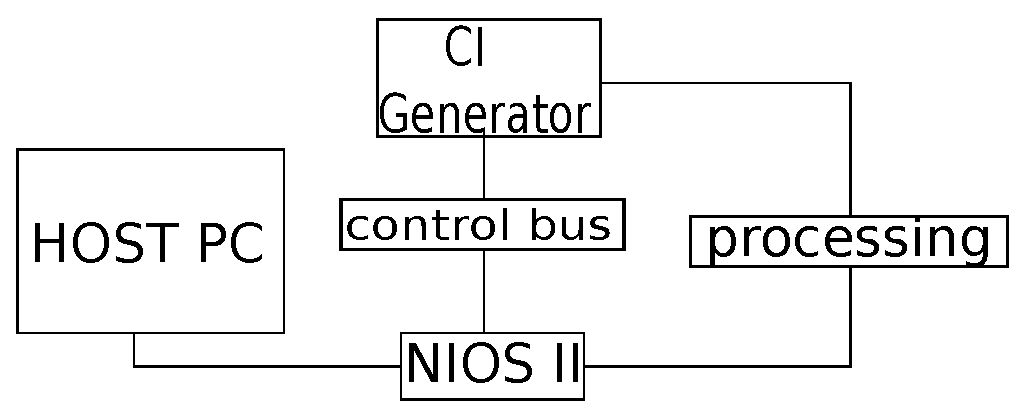
\includegraphics[width=6cm]{nios.eps}
\label{nios}} \hspace{0.5cm}
\subfigure[Schematic]{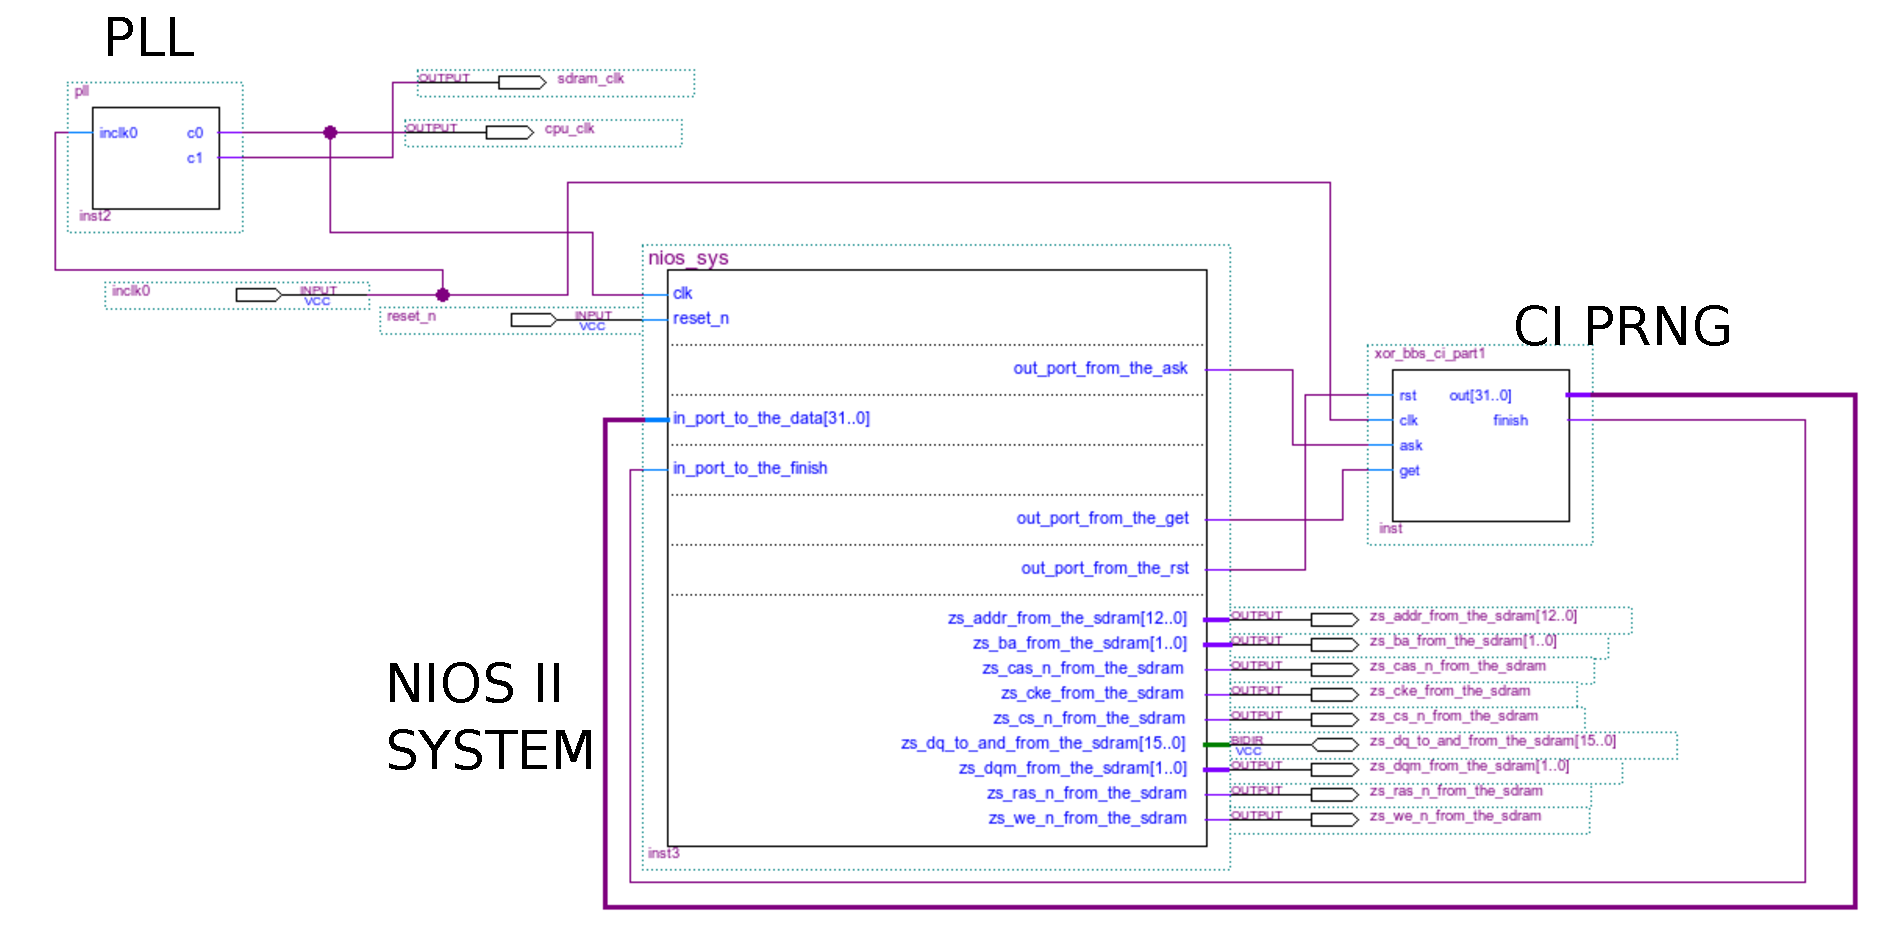
\includegraphics[width=\columnwidth]{nios2.eps}
\label{nios2}} \hspace{0.5cm}
\caption{NIOS II setting in FPGA}
\label{Spatial MSCs and LSCs of Lena}
\end{figure}

\section{Software Implementation Experiment Protocol}
In this section, an information hiding application based on chaotic iterations is represented, a watermark is encrypted and embedded into a cover image using the scheme presented in the previous section and CIPRNG. The Version 4 CI PRNG (BBS, XORshift) is chosen, since its cryptographically secure property, good statistical performance and high efficiency.  The carrier image is the well-known Lena, which is a 256 grayscale image, and the watermark is the $64\times 64$ pixels binary image depicted in Figure~\ref{Original images}.


\begin{figure}[!t]
\centering
\subfigure [The original image]{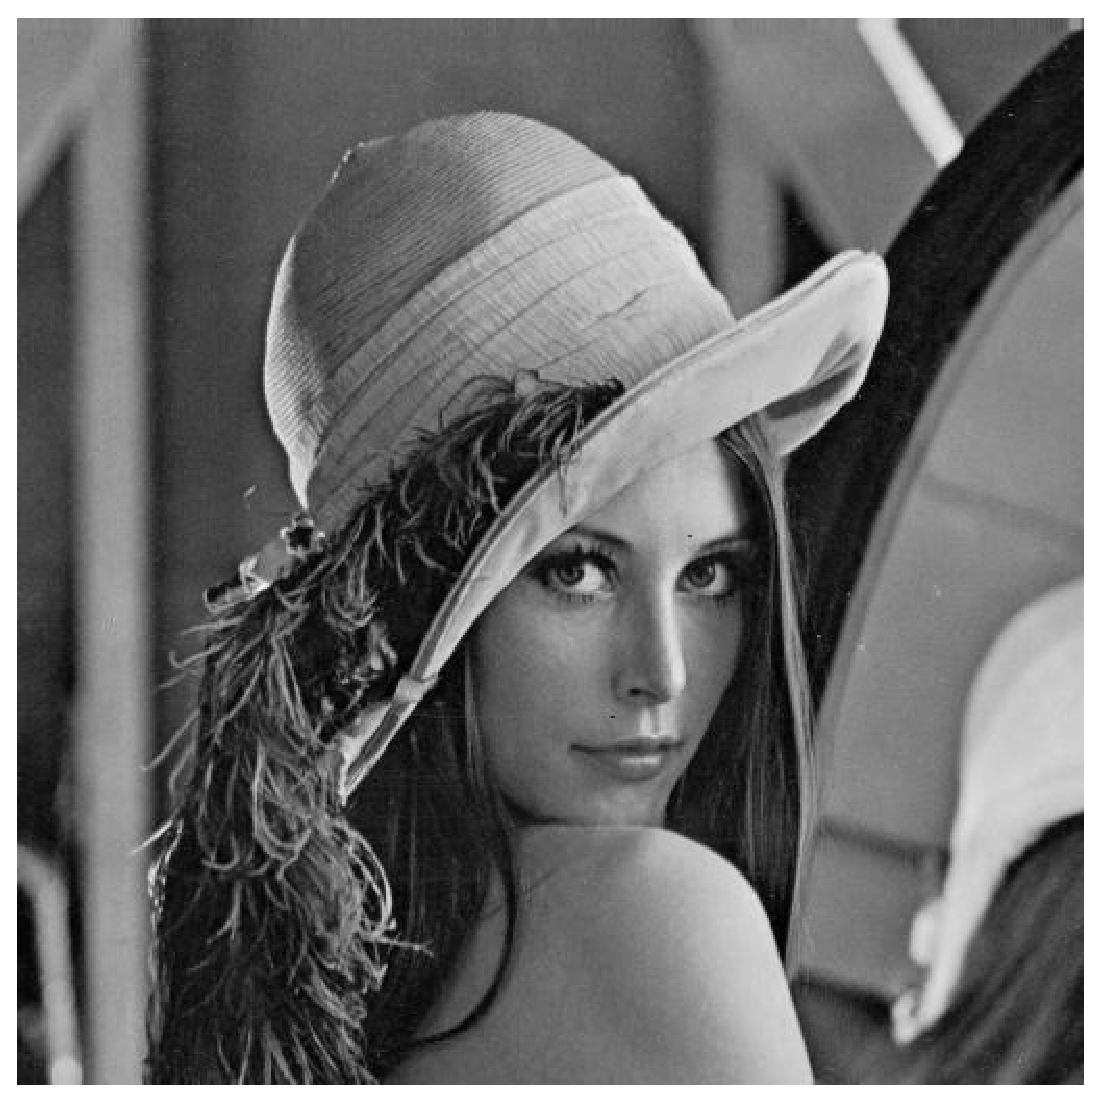
\includegraphics[scale=0.23]{lena512.eps}}
\hfil
\subfigure[The watermark]{
\includegraphics[scale=0.4]{invader1.eps}%
}
\caption{Original images}
\label{Original images}
\end{figure}


\begin{figure}
\centering
\subfigure[Output image]{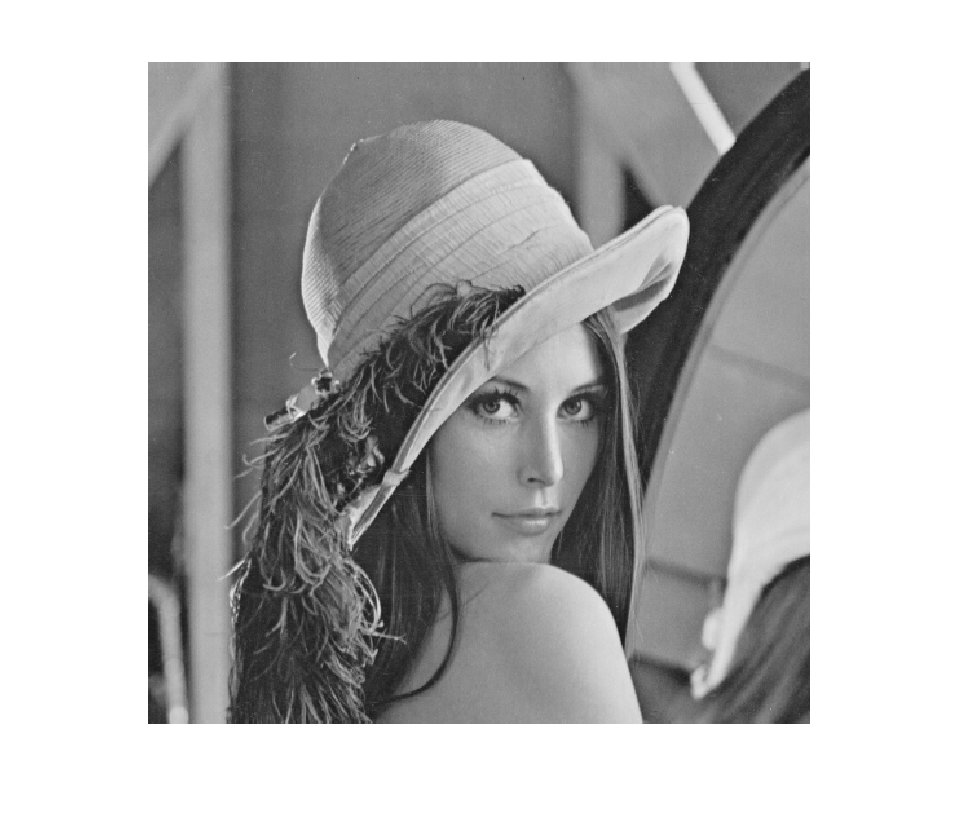
\includegraphics[scale=0.4]{output_lena.eps}}
\subfigure[Difference]{
\includegraphics[scale=0.4]{diff.eps}}
\caption{The output of watermarking application}
\label{java_end}
\end{figure}
We program our application via JAVA~\cite{java}, where The watermark is encrypted by using chaotic iterations: the initial state $x^{0}$ is the watermark, considered as a boolean vector, the iteration function is the vectorial logical negation, and the chaotic strategy $(S^{k})_{k\in \mathds{N}}$ is defined with Version 4 CIs(BBS, XORshift), where initial parameters constitute the secret key and $N=64$. The JAVA application is working as a windows interface(shown if Figure ~\ref{java_start}), firstly the embed file is chosen as Figure~\ref{java_chosen}, then we choose the image which used to carry the contents (Figure~\ref{java_image}), lastly after processing, the output image is produced, and in Figure~\ref{java_end}, the difference between original image and encrypted image is also shown.

\begin{figure}
\centering
\subfigure [The start windows of JAVA watermarking Application]{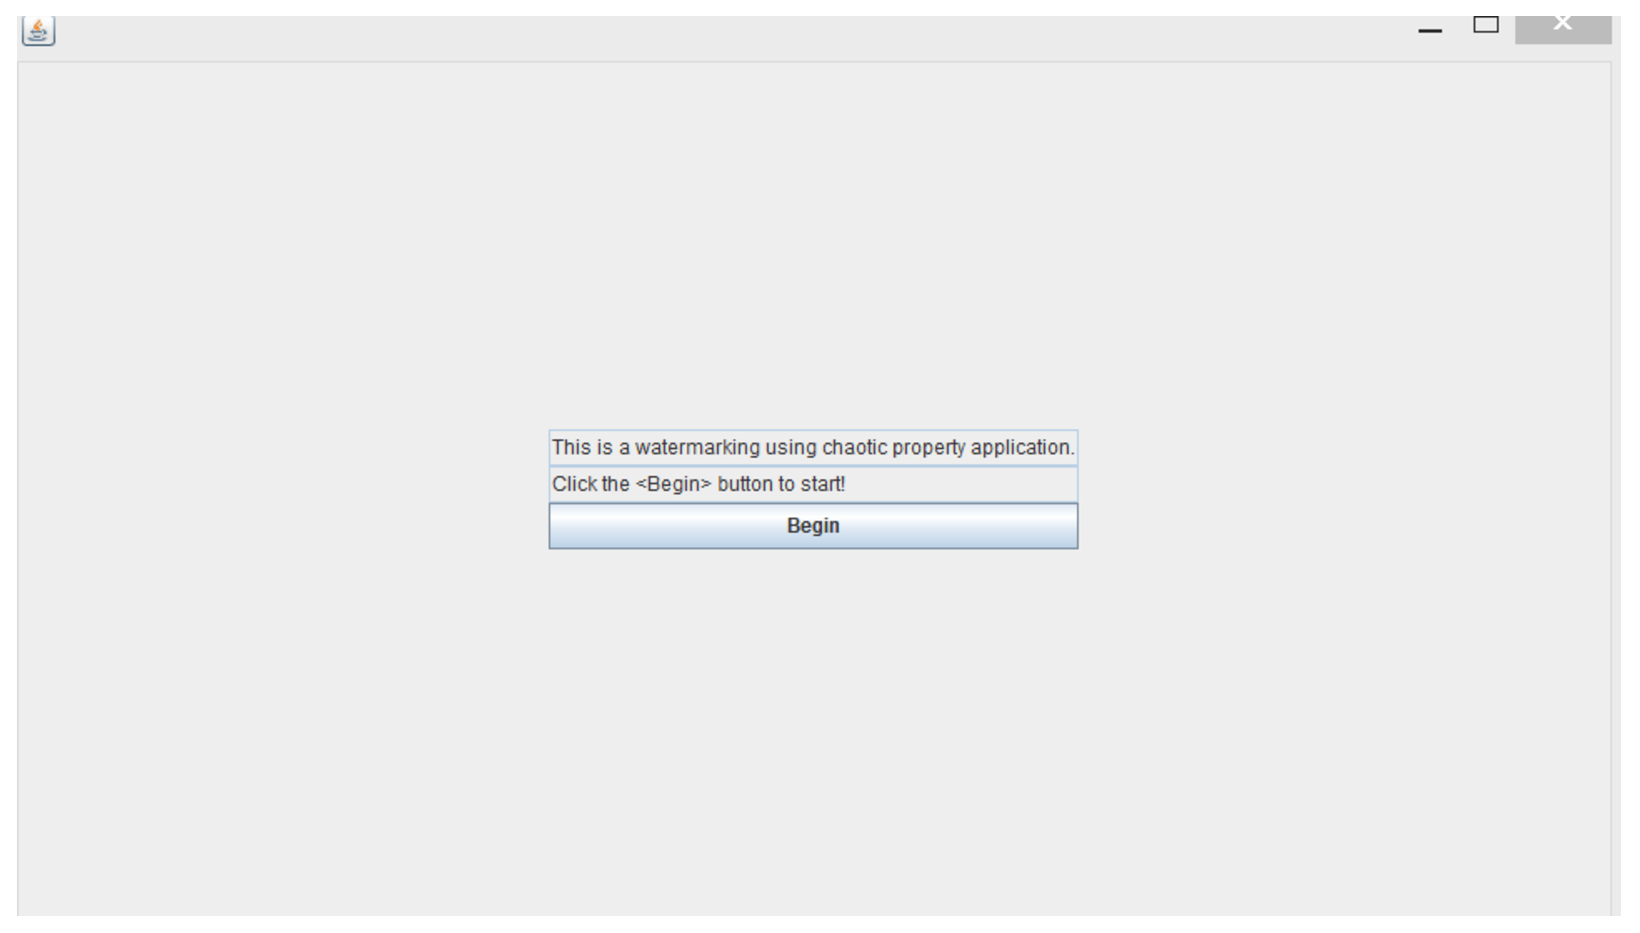
\includegraphics[scale=0.3]{start.eps}}
\label{java_start}
\subfigure [Choosing the contends to be embed]{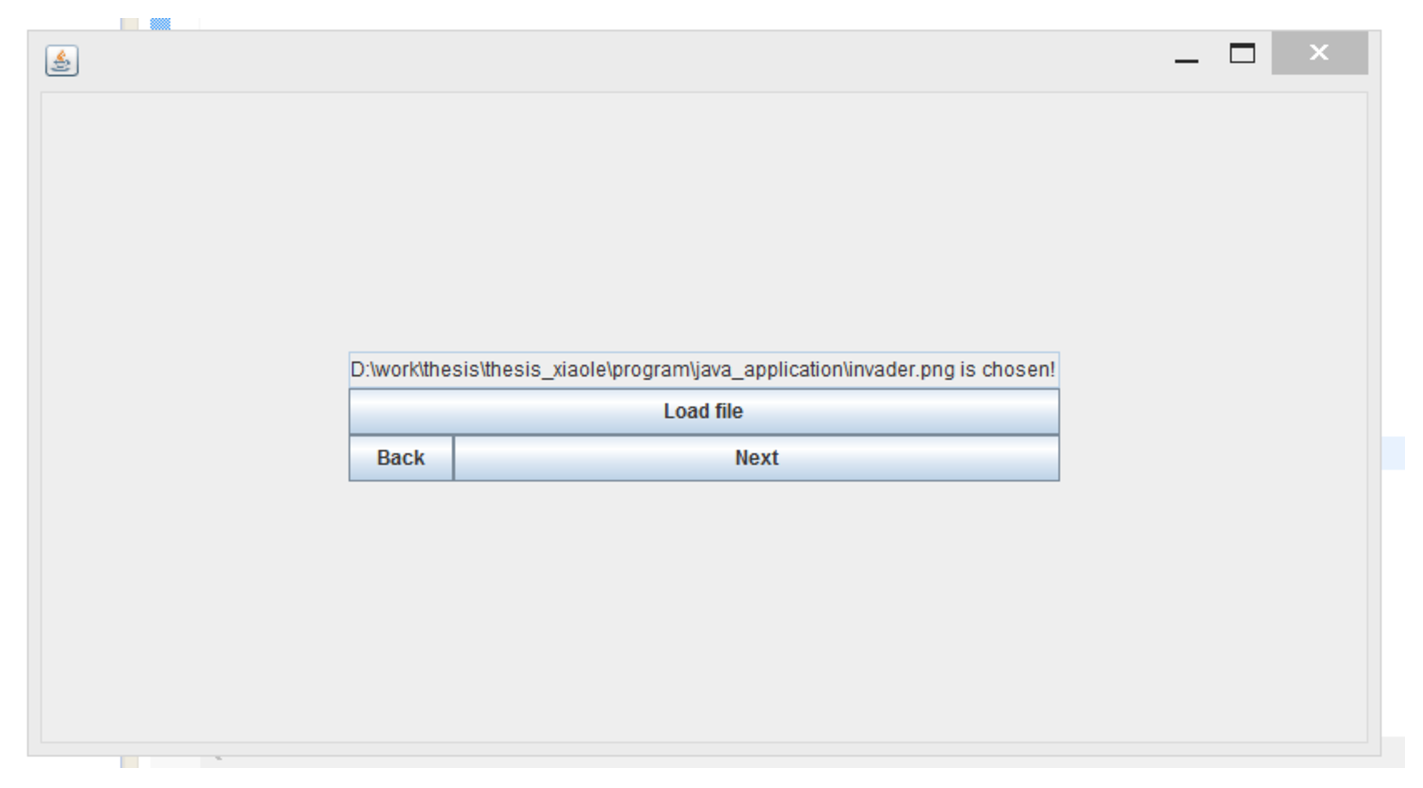
\includegraphics[scale=0.3]{chooseFile.eps}}
\label{java_chosen}
\subfigure [Choosing the contends to be embed]{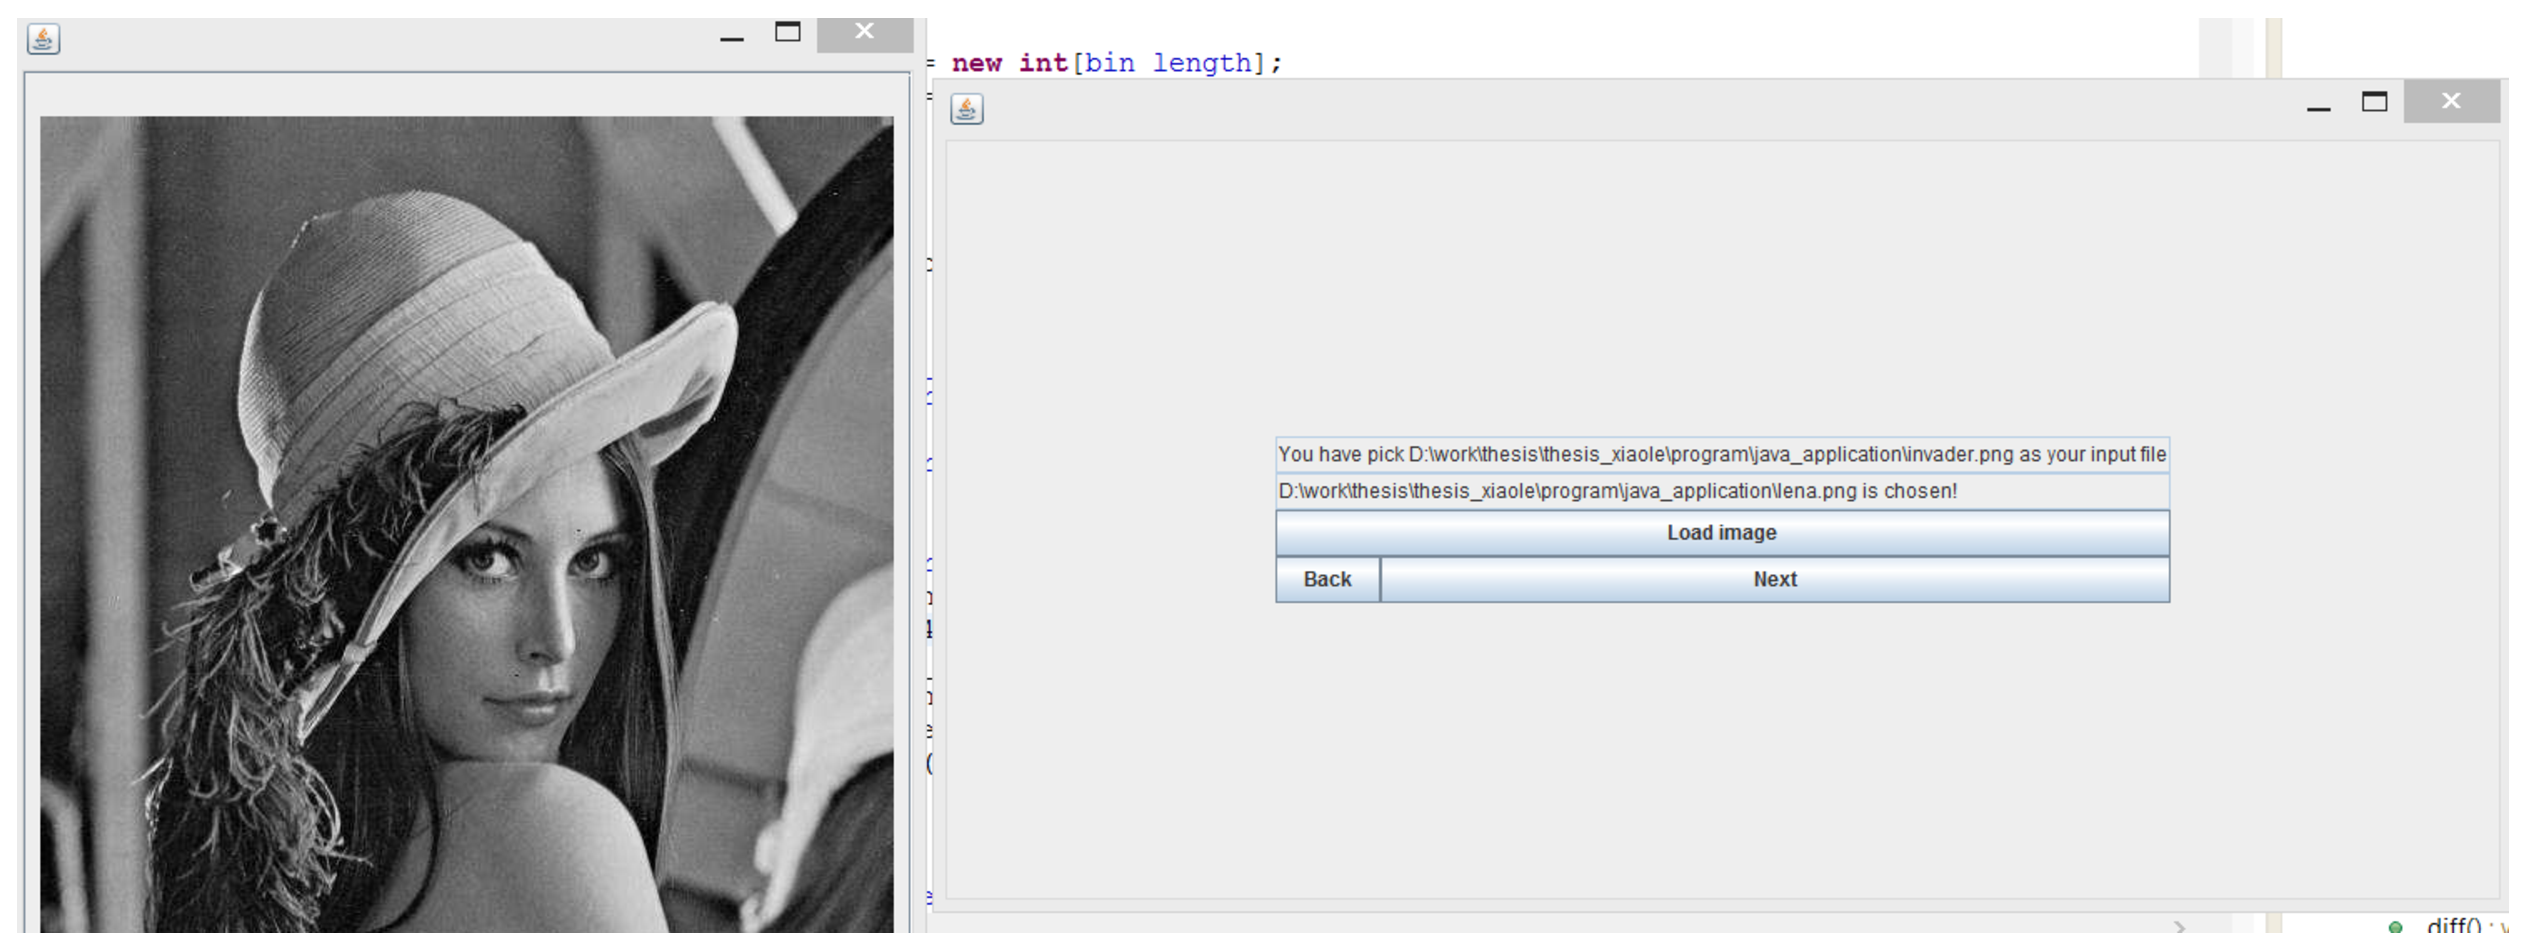
\includegraphics[scale=0.3]{chooseImage.eps}}
\label{java_image}
\caption{Java application for watermarking based on chaotic iteration generator}
\label{java application}
\end{figure}



\section{Hardware Implementation Experiment Protocol}
In this section, the watermarking algorithm based on the chaotic PRNG presented above by FPGA is given, as an 
illustration of use of this PRNG based on CI.

Here the 32-bit embedded-processor architecture designed specifically for the Altera family of FPGAs 
is applied to execute this application. Nios II incorporates many enhancements over the original 
Nios architecture, making it more suitable for a wider range of embedded computing applications, 
from DSP to system-control~\cite{nios}. Figure~\ref{nios} shows the structure of this application, 
the NIOS II system can read the image from the HOST computer side, then according the control bus 
to operate the CI generator to produce random bits, and at last the processing results are transmitted back into 
the host. In Figure~\ref{nios2}, the NIOS II is using the most powerful version the CYCLONE II can support(NIOS II/f), 
then $4$ KB on chip memory and $16$ MB SDRAM are set, the $PLL$ device is used to enhance the clock frequency from $50$ 
to $200$ MHz, the data bus connects NIOS II system and generator is in 32 bits.


\section{Robustness evaluation}

In what follows, the embedding domain is the spatial domain, Version 4 CI(BBS,XORshift) with parameters $....$ has been used to encrypt the watermark, MSCs are the four first bits of each pixel (useful only in case of authentication), and LSCs are the three next bits.

To prove the efficiency and the robustness of the proposed algorithm, some
attacks are applied to our chaotic watermarked image. For each attack, a
similarity percentage with the watermark is computed, this percentage is the
number of equal bits between the original and the extracted watermark, shown
as a percentage. Let us notice that a result less than or equal to $50\%$
implies that the image has probably not been watermarked.

\subsubsection{Zeroing attack}

In this kind of attack, a watermarked image is zeroed, such as in Figure \ref{fig:LenaAttack}(a). In this case, the results in Table 1 have been obtained.

\begin{figure}[htb]
\begin{minipage}[b]{.48\linewidth}
  \centering
 \centerline{\epsfig{figure=lennaDecoupe100px,width=3.3cm}}
  \centerline{(a) Cropping attack}
\end{minipage}
\hfill
\begin{minipage}[b]{0.48\linewidth}
  \centering
 \centerline{\epsfig{figure=lennaTourne25d.eps,width=3.3cm}}
  \centerline{(b) Rotation attack}
\end{minipage}
\caption{Watermarked Lena after attacks.}
\label{fig:LenaAttack}
\end{figure}




\begin{center}
\begin{footnotesize}
\begin{tabular}{|c|c||c|c|}
\hline
\multicolumn{2}{|c||}{UNAUTHENTICATION}  & \multicolumn{2}{c|}{AUTHENTICATION}\\ 
\hline
Size (pixels) & Similarity & Size (pixels) & Similarity \\
 \hline
10 & 99.31\% & 10 & 92.34\% \\
50 & 98.55\% & 50 & 57.11\% \\
100 & 92.40\% & 100 & 54.42\% \\
200 & 71.01\% & 200 & 50.93\% \\
\hline
\end{tabular}
\end{footnotesize}\\
\vspace{0.5cm}
\textbf{Table. 1}. ~Cropping attacks
\end{center}


In Figure \ref{fig:Dechiffrement_invader}, the decrypted watermarks are shown after a crop of 50 pixels and after a crop of 10 pixels, in the authentication case.

\begin{figure}[htb]
\begin{minipage}[b]{1.0\linewidth}
  \centering
 \centerline{\epsfig{figure=invaderDechiffreDecoupe100px.eps,width=2cm}}
  \centerline{(a) Unauthentication ($50\times 50$).}
\end{minipage}
%
\begin{minipage}[b]{.48\linewidth}
  \centering
 \centerline{\epsfig{figure=invaderDechiffreDecoupeAuth100px.eps,width=2cm}}
  \centerline{(b) Authentication  ($50\times 50$).}
\end{minipage}
\hfill
\begin{minipage}[b]{0.48\linewidth}
  \centering
 \centerline{\epsfig{figure=invaderDechiffreDecoupeAuth50px.eps,width=2cm}}
  \centerline{(c) Authentication  ($10\times 10$).}
\end{minipage}
%
\caption{Extracted watermark after a cropping attack.}
\label{fig:Dechiffrement_invader}
%
\end{figure}


By analyzing the similarity percentage between the original and the
extracted watermark, we can conclude that in case of unauthentication, the
watermark still remains after a zeroing attack: the desired robustness is
reached. It can be noticed that zeroing sizes and percentages are rather
proportional.

In case of authentication, even a small change of the carrier image (a crop
by $10\times 10$ pixels) leads to a really different extracted watermark.
In this case, any attempt to alter the carrier image will be signaled, the
image is well authenticated.
\begin{center}
\begin{footnotesize}
\begin{tabular}{|c|c||c|c|}
\hline
\multicolumn{2}{|c||}{UNAUTHENTICATION}  & \multicolumn{2}{c|}{AUTHENTICATION}\\ 
\hline
Angle (degree) & Similarity & Angle (degree) & Similarity \\
 \hline
2 & 97.31\% & 2 & 74.45\% \\
5 & 94.02\% & 5 & 63.36\% \\
10 & 89.98\% & 10 & 52.77\% \\
25 & 80.84\% & 25 & 52.03\% \\
\hline
\end{tabular}
\end{footnotesize}\\
\vspace{0.5cm}
\textbf{Table. 2}. ~Rotation attacks

\end{center}

\subsubsection{Rotation attack}

Let $r_{\theta }$ be the rotation of angle $\theta $ around the center $%
(128, 128)$ of the carrier image. So, the transformation $r_{-\theta }\circ
r_{\theta }$ is applied to the watermarked image, which is altered as in Figure \ref{fig:LenaAttack}. The results in Table 2 have been obtained.




The same conclusion as above can be declaimed: this watermarking method
satisfies the desired properties.

\subsubsection{JPEG compression}

A JPEG compression is applied to the watermarked image, depending on a
compression level. Let us notice that this attack leads to a change of
the representation domain (from spatial to DCT domain). In this case, the results in Table 3 have been obtained.

\begin{center}
\begin{footnotesize}
\begin{tabular}{|c|c||c|c|}
\hline
\multicolumn{2}{|c||}{UNAUTHENTICATION}  & \multicolumn{2}{c|}{AUTHENTICATION}\\ 
\hline
Compression & Similarity & Compression & Similarity \\
 \hline
2 & 85.92\% & 2 & 58.42\% \\
5 & 70.45\% & 5 & 53.11\% \\
10 & 64.39\% & 10 & 51.02\% \\
20 & 53.94\% & 20 & 50.03\% \\
\hline
\end{tabular}
\end{footnotesize}\\
\vspace{0.5cm}
\textbf{Table. 3}. ~JPEG compression attacks
\end{center}

A very good authentication through JPEG attack is obtained. As for the
unauthentication case, the watermark still remains after a compression level
equal to 10. This is a good result if we take into account the fact that we
use spatial embedding.

\subsubsection{Gaussian noise}

Watermarked image can be also attacked by the addition of a Gaussian noise, depending on a standard deviation. In this case, the results in Table 4 have been obtained.


\begin{center}
\begin{footnotesize}
\begin{tabular}{|c|c||c|c|}
\hline
\multicolumn{2}{|c||}{UNAUTHENTICATION}  & \multicolumn{2}{c|}{AUTHENTICATION}\\ 
\hline
Standard dev. & Similarity & Standard dev. & Similarity \\
 \hline
1 & 81.00\% & 1 & 56.50\% \\
2 & 77.18\% & 2 & 51.92\% \\
3 & 67.01\% & 3 & 52.82\% \\
5 & 59.28\% & 5 & 51.76\% \\
\hline
\end{tabular}
\end{footnotesize}\\
\vspace{0.5cm}
\textbf{Table. 4}. ~Gaussian noise attacks
\end{center}


Once again we remark that good results are obtained, especially if we keep in
mind that a spatial representation domain has been chosen.




\bibliographystyle{plain}
\bibliography{Thesis}
\end{document}
